
\documentclass[a4paper,11pt]{amsart}
\oddsidemargin  0.4 cm
\evensidemargin 0.4 cm
\textwidth     15.16 cm
\headsep        0.8 cm

\usepackage{dsfont}
\usepackage{amsmath,amsthm,amssymb,tabu,stmaryrd}
\usepackage{mathtools,comment}
\usepackage[all]{xy}
\usepackage[usenames, dvipsnames]{color}
\usepackage{listings} %for copy-pasting code
\usepackage{graphicx}
\usepackage[table]{xcolor}
\usepackage{hyperref, url}
\hypersetup{
	colorlinks=true,
	linkcolor=OliveGreen,
	filecolor=magenta,
	urlcolor=darkgray,
	citecolor=OliveGreen
}
\usepackage[noadjust]{cite}
\usepackage{tikz-cd}
\usepackage{tikz}
\usetikzlibrary{shapes.geometric,calc,arrows,positioning}
\usepackage{enumitem}
\usetikzlibrary{shapes.geometric,calc,arrows}
\usepackage{multirow}
\usepackage{skak}
\usepackage[normalem]{ulem}
\usepackage[makeroom]{cancel}

%%% For the external link icon %%%
\RequirePackage{fontawesome}

%%%Vakil font%%%
%\usepackage{mathpazo}
%\usepackage{euler}
%%%%%%%%%%%%%%%%

\tikzstyle{startstop} = [rectangle, rounded corners, minimum width=1.7cm, minimum height=0.7cm,text centered, draw=black, fill=gray!20]
\tikzstyle{io} = [trapezium, trapezium left angle=75, trapezium right angle=105, minimum width=1.3cm, minimum height=0.7cm, text centered, draw=black, inner sep=8]
\tikzstyle{process} = [rectangle, minimum width=1.3cm, minimum height=0.7cm, text centered, draw=black]
\tikzstyle{decision} = [diamond, minimum width=1.3cm, minimum height=0.7cm, text centered, draw=black, aspect=2, inner sep=2]
\tikzstyle{arrow} = [->,>=stealth,line width=0.5mm]




\usepackage[iso-8859-7]{inputenc}

%%%Theorems%%%
\newtheorem{introductiontheorem}{Theorem}
\newtheorem{theorem}{Theorem}[section]
\newtheorem{corollary}[theorem]{Corollary}
\newtheorem{lemma}[theorem]{Lemma}
\newtheorem{proposition}[theorem]{Proposition}
\newtheorem{remark}[theorem]{Remark}
\newtheorem{definition}[theorem]{Definition}
\newtheorem{example}[theorem]{Example}
\newtheorem{construction}[theorem]{Construction}
\newtheorem{notation}[theorem]{Notation}
\newtheorem{exercise}[theorem]{Exercise}
\newtheorem{setup}[theorem]{Setup}



%%%Shortcut Commands%%%
\def\ker{\operatorname{ker}}
\def\coker{\operatorname{coker}}
\def\im{\operatorname{im}}
\def\dim{\operatorname{dim}}
\def\codim{\operatorname{codim}}
\def\rank{\operatorname{rank}}
\def\id{\operatorname{id}}
\def\deg{\operatorname{deg}}
\def\wt{\operatorname{wt}}
\def\mult{\operatorname{mult}}
\def\g{\operatorname{g}}
\def\det{\operatorname{det}}
\def\Div{\operatorname{Div}}
\def\WDiv{\operatorname{WDiv}}
\def\NE{\operatorname{NE}}
\def\NEb{\overline{\operatorname{NE}}}
\def\NS{\operatorname{NS}}
\def\Exc{\operatorname{Exc}}
\def\Supp{\operatorname{Supp}}
\def\Bl{\operatorname{Bl}}
\def\mult{\operatorname{mult}}
\def\Pic{\operatorname{Pic}}
\def\Eff{\operatorname{Eff}}
\def\Pseff{\operatorname{Pseff}}
\def\Mov{\operatorname{Mov}}
\def\Nef{\operatorname{Nef}}
\def\Cone{\operatorname{Cone}}
\def\Proj{\operatorname{Proj}}
\def\Spec{\operatorname{Spec}}
\def\Sing{\operatorname{Sing}}
\def\BirMori{\operatorname{BirMori}}
\DeclareMathOperator{\BirMoriB}{\mathbf{BirMori}}
\def\Bir{\operatorname{Bir}}
\def\Aut{\operatorname{Aut}}
\def\Autzero{\mathrm{Aut}^\circ}
\def\divv{\operatorname{div}}
\def\PGL{\operatorname{PGL}}
\def\GL{\operatorname{GL}}
\def\PSO{\operatorname{PSO}}
\def\SO{\operatorname{SO}}
\def\Orth{\operatorname{O}}
\def\Hom{\operatorname{Hom}}
\def\Cr{\operatorname{Cr}}
\def\cha{\operatorname{char}}
\def\diag{\operatorname{diag}}
\def\det{\operatorname{det}}
\def\disc{\operatorname{disc}}
\def\cent{\operatorname{cent}}
\def\Mor{\operatorname{Mor}}
\def\Sym{\operatorname{Sym}}
\def\inter{\operatorname{int}}
\def\ev{\operatorname{ev}}
\def\Ker{\operatorname{Ker}}
\def\Amp{\operatorname{Amp}}

\newcommand{\x}{\chi}

\newcommand{\OO}{\mathcal{O}}
\newcommand{\II}{\mathcal{I}}
\newcommand{\HH}{\mathcal{H}}
\newcommand{\Hh}{\mathcal{H}}
\newcommand{\Cc}{\mathcal{C}}
\newcommand{\Aa}{\mathcal{A}}
\newcommand{\Pp}{\mathcal{P}}
\newcommand{\Tt}{\mathcal{T}}

\renewcommand{\AA}{\mathbb{A}}
\newcommand{\NN}{\mathbb{N}}
\newcommand{\ZZ}{\mathbb{Z}}
\newcommand{\QQ}{\mathbb{Q}}
\newcommand{\RR}{\mathbb{R}}
\newcommand{\CC}{\mathbb{C}}
\newcommand{\PP}{\mathbb{P}}
\renewcommand{\FF}{\mathbb{F}}
\newcommand{\GG}{\mathbb{G}}
\newcommand{\kk}{\textbf{k}}
\newcommand{\KK}{\mathbb{K}}


\newcommand{\isom}{\cong}
\newcommand{\defeq}{\vcentcolon=}
\newcommand{\map}{\smash{\xymatrix@C=0.5cm@M=1.5pt{ \ar[r]& }}}
\newcommand{\rmap}{\dashrightarrow}
%\newcommand{\rmap}{\smash{\xymatrix@C=0.5cm@M=1.5pt{ \ar@{-->}[r]& }}}
\newcommand{\psmap}{\smash{\xymatrix@C=0.5cm@M=1.5pt{ \ar@{..>}[r]& }}}




\newcommand{\sok}[1]{{\color{OliveGreen}#1}}


\title{Algebraic surfaces \& the Sarkisov Program.}
\author{}
\date{\today}

\begin{document}


%\begin{abstract}
%	The plan of the course is to touch upon the following topics:
%	\begin{enumerate}
%		\item Reminders from surface theory: intersection theory, blowups, linear systems, resolution of birational maps, etc.
%		\item Vanishing theorems and Castelnuovo's contraction theorem.
%		\item Short overview of the Minimal Model Program (MMP) in dimension 2.
%		\item Mori fiber spaces and the Sarkisov Program.
%		\item Ample and semiample models.
%		\item Geography of ample models.
%		\item Proof of the Sarkisov program.
%		\item Application: generators of $\Cr_2(\CC)$.
%		\item Connections to finite generation of adjoint rings.
%	\end{enumerate}
%	Main references: \cite{Cremona}, \cite{Matsuki}.
%\end{abstract}

\maketitle

\tableofcontents

\section{Reminders from surface theory}


\subsection{Intersection Theory}

\begin{theorem}
	Let $S$ be a smooth projective surface.
	There exists a unique symmetric bilinear paring 
	\[
	\begin{array}{ccc}
		\Div(S) \times \Div(S) & \to & \ZZ\\
		(D,C) 	& \mapsto & D\cdot C
	\end{array}
	\]
	with the following properties:
	\begin{enumerate}
		\item\label{it:inters1} if $D$ and $C$ are effective divisors meeting transversally, then 
		\[
		D\cdot C = \#(D \cap C);
		\]
		{\small (even if $D$ and $C$ don't meet transversally, and as long as they have no common components, we can still define $D\cdot C$ by summing up their points of intersection but keeping in mind the \emph{"degree of tangency"} at each point.)}
		\item\label{it:inters2} if $C_1 \sim C_2$ then $D\cdot C_1 = D\cdot C_2$, for every $D \in \Div(X)$.
	\end{enumerate}
\end{theorem}

\begin{proof}[Sketch of proof]
	The idea is to start by defining the product only on effective divisors intersecting transversally as in \eqref{it:inters1}.
	If two effective divisors $D, C$ don't intersect transversally show that we can find $C\sim \sum a_i C_i$ so that $D$ and $C_i$ intersect transversally;
	then define 
	\[
	D \cdot C \defeq \sum a_i D\cdot C_i.
	\]
	Note that the $a_i$ don't have to be positive.
	Finally extend by linearity to non-effective divisors too.
	
	For details see \cite[Chapter V, Theorem 1.1]{Hartshorne}.
\end{proof}


\begin{definition}
	Two divisors $D_1, D_2$ are called \textbf{numerically equivalent} if
	\[
	D_1 \cdot C = D_2 \cdot C, \, \text{ for all curves $C \subset S$}.
	\]
	We denote that by $D_1 \equiv D_2$, and write $N^1(S) = \{\Div(S)/\equiv\}\otimes \RR$ for the space of divisors up to numerical equivalence.
	
	Two curves $C_1, C_2$ are called \textbf{numerically equivalent} if
	\[
	D \cdot C_1 = D \cdot C_2, \, \text{ for all $D \in \Div(S)$}.
	\]
	We denote that by $C_1 \equiv C_2$, and write $N_1(S) = \{Z_1(S)/\equiv\}\otimes \RR$ for the space of $1$-cycles up to numerical equivalence.
	
	We define the \textbf{cone of curves} $\NE(S)$ to be the cone in $N_1(S)$ spanned by curves. 
	Its closure $\NEb(S)$ is called the \textbf{Mori cone} of $S$.
	
	The vector spaces $N^1(S)$ and $N_1(S)$ are dual to one another (via the intersection pairing), and so $\dim N^1(S) = \dim N_1(S)$.
	Moreover, their dimension is finite and called the \textbf{Picard rank} $\rho(S)$ of $S$.
\end{definition}



\begin{theorem}[{Numerical criteria for ampleness}]\label{thm:NM}
	For a divisor $D$ on a smooth surface $S$ the following are equivalent:
	\begin{enumerate}
		\item\label{it:ampleness1} $D$ is ample;
		\item\label{it:ampleness2} $D^2 > 0$ and $D\cdot C > 0$ for any curve $C \subset S$;
		\item\label{it:ampleness3} $D\cdot z >0$ for any class $z \in \NEb(S)$.
	\end{enumerate}
	
	The equivalences \eqref{it:ampleness1} $\Leftrightarrow$ \eqref{it:ampleness2} and \eqref{it:ampleness1} $\Leftrightarrow$ \eqref{it:ampleness3} are known as \textbf{Nakai-Moischezon} and \textbf{Kleiman} criteria for ampleness respectively.
\end{theorem}

This shows that ampleness is a numerical property.
Nefness is a slight weakening of ampleness:

\begin{definition}
	A divisor is called \textbf{nef} if $D\cdot C \geq 0$ for every curve in $S$.
\end{definition}




\subsection{How blowups change intersections}

\begin{definition}\label{def:pull-push}
	Let $f\colon T \to S$ be a morphism of surfaces.
	
	If $D \in \Div(S)$ be a divisor cut out locally by the equations $\{(U_i,h_i)\}$ we define the \textbf{pullback} of $D$ as
	\[
	f^*D \defeq \{f^{-1}(U_i), h_i\circ f\}.
	\]
	
	If $C$ is a curve in $T$ we define the \textbf{pushforward} of $C$ as
	\[
	f_*C \defeq 
	\left\{
	\begin{array}{ll}
			d \cdot f(C), & \text{ if $f(C)$ is a curve;}\\
		0, & \text{ if $f(C)$ is a point,}	
	\end{array}	
	\right.
	\]
	where $d$ is the is the degree of $f|_C$.
	
	These notions satisfy the \textbf{pull-push formula}:
	\[
	f^*D \cdot C = D \cdot f_*C.
	\]
\end{definition}

\begin{definition}
	We define the \textbf{blowup of $\AA^2$ at the origin} to be
	\[
	\Bl_0\AA^2 \defeq \{(x_0,x_1),(u_0:u_1) \in \AA^2 \times \PP^1 \, | \, x_0u_1 - x_1u_0 = 0\}
	\]
	together with the projection to the first factor $\Bl_0\AA^2 \to \AA^2$.
	
	Let $S$ be a smooth surface and $p\in S$ a point.
	We define \textbf{the blowup of $S$ along $p$} by choosing an (analytic) neighbourhood $p \in U \subset S$ so that $(p,U) \isom (0,\AA^2)$, blowing up $U$ along $p$ and glueing accordingly.
\end{definition}

\begin{proposition}\label{prop:blp}
	Let $S$ be a smooth projective surface and $f\colon T \to S$ the blowup along a point $p$ with exceptional divisor $E$.
	Then 
	\begin{enumerate}
		\item\label{it:bl1} $f^*D\cdot f^*C = D\cdot C$ for any $D,C \in \Div(S)$;
		\item\label{it:bl2} $f^*C = \tilde{C} + mE$, where $m$ is the multiplicity of $C$ at $p$, in particular $\Pic(T) = f^*\Pic(S) \oplus \ZZ E$;
		\item\label{it:bl3} $K_T = f^*K_S + E$;
		\item\label{it:bl4} $E \isom \PP^1$ and $E^2 = -1$.
	\end{enumerate}
\end{proposition}

\begin{proof}[Sketch of proof]
	\eqref{it:bl1} is by Serre's moving lemma: move $D$ and $C$ away from $p$; the blowup changes nothing away from $p$.
	\eqref{it:bl2} and \eqref{it:bl3} are local calculations: pullback the equation of a curve/differential form.
	As for \eqref{it:bl4} work again locally: let $L_1, L_2$ be two lines through $0 \in \AA^2$; we have
	\[
	1 = L_1 \cdot L_2 = f^*(L_1)\cdot f^*(L_2) = \tilde{L}_1 \cdot \tilde{L}_2 + \tilde{L}_1 \cdot E + \tilde{L}_2\cdot E + E^2 = 2 + E^2.
	\]
\end{proof}

\begin{remark}\label{rem:negCurves}\leavevmode
	\begin{enumerate}
		\item\label{it:negCurves1} If $D$ and $C$ are effective divisors, then $D\cdot C<0$ implies that $C \subset D$.
		\item\label{it:negCurves2} In particular, if $C^2<0$ for an irreducible curve, then $h^0(S,\OO_S(C)) = 1$;
		that is curves of negative self intersection are \href{https://s-zikas.github.io/site/pics/-1curve.jpg}{unique} in their linear system.
		\item Proposition \ref{prop:blp}\eqref{it:bl2} gives us a way to turn incomplete linear systems into complete ones.
	\end{enumerate}
\end{remark}


\subsection{Resolution of (bi)rational maps}\leavevmode




\begin{minipage}{.8\textwidth}
\hypertarget{rem:maps}{\underline{Reminder - \emph{Maps to $\PP^n$}}}:
for a divisor $D \in \Div(S)$ we define its \textbf{global sections} as:
\begin{align*}
	H^0(S,D) &\defeq \{ f \in \kk(S) \,|\, D'\defeq \divv(f) + D \geq 0 \} \\
	& \phantom{:}= \{D' \in \Div(X) \, | \, D' \geq 0 \text{ and } D \sim D'\}.
\end{align*}
Essentially sections of a divisor are rational functions that are allowed to have poles as most on $D$.
Note that $H^0(S,D)$ is a $\kk$-vector space;
a subspace $V \leq H^0(S,D)$ is called a \textbf{linear system};
if $V = H^0(S,D)$ we call it \textbf{the complete linear system of $D$}.
From now on, whenever we talk about sections of a divisor, we will freely interchange between the rational functions and the corresponding effective divisor.
Given a linear system $V$ we define its \textbf{fixed part} $F$ to be the biggest divisor that is contained in \emph{every} element of $V$.

\vspace{.1cm}

There is a bijection 
\[
\begin{array}{ccc}
	\big\{ \text{Rational maps to $\PP^n$} \big\} & \leftrightarrow & \big\{ \text{Linear systems with no fixed part} \}\\
	f\colon S \rmap \PP^n & \mapsto & \langle f^*\{x_i =0\}, \, 0\leq i \leq n \rangle \\
	f =  (f_0:\ldots :f_n) & \mapsfrom & \langle f_0,\dots, f_n \rangle = V.
\end{array}
\]
The map $f$ will fail to be a morphism precisely when $f_0, \dots, f_n$ share a common zero;
equivalently where the divisors $D_i$ intersect.
We say that a divisor is \textbf{base point free (bpf)} if its complete linear system defines a morphism.
We say that it is \textbf{semiample} if a multiple of it is bpf.

By Remark \ref{rem:negCurves}\eqref{it:negCurves1}, on the right hand side of the bijection we only care for divisors that are nef.
However not all nef divisors correspond to morphisms (see Exercise \ref{exer:cubicsThought8and9})
\end{minipage}


\begin{example}
	Consider $D = \{x_0 = 0\}$ as a divisor on $\PP^2$.
	Then 
	\begin{align*}
		H^0(S,D) &= \left\{ \frac{l}{x_0} \in \kk(S) \,\middle|\, l \in \kk[x_0,x_1,x_2]_1 \right\}  = \left\langle \frac{x_0}{x_0}, \frac{x_1}{x_0}, \frac{x_2}{x_0} \right\rangle.
	\end{align*}
	 
	
	Consider the rational map	
	\[
	\begin{array}{ccc}
		\PP^2 & {\smash{\xymatrix@C=0.5cm@M=1.5pt{ \ar@{-->}[r]^f& }}}& \PP^1\\
		(x_0:x_1:x_2) & \mapsto & \left(\frac{x_0}{x_0} : \frac{x_0+x_1}{x_0}\right) =  (x_0:x_0+x_1)
	\end{array}
	\]
	not defined at the point $p = (0:0:1)$;
	this is precisely the point of intersection of the two lines $l_0 = \{x_0 = 0\}$ and $l_1 = \{x_0 + x_1 = 0\}$.
	We will fix that by blowing up $p$ and thus disconnecting the lines.
	
	The blowup $\pi\colon S \to \PP^2$ of $\PP^2$ at $p$ is given by
	\[
	S  = \left\{(x_0:x_1:x_2),(u_0:u_1) \in \PP^2\times \PP^1 \,|\, x_0u_1 - x_1u_0 = 0 \right\}.
	\]
	We will work locally at the open chart $U_{2,0} = \{x_2 = u_0 = 1\}$.
	We have the isomorphism
	\[
	\begin{array}{ccc}
		\AA^2 & \to & U_{2,0}\\
		(X_0,X_1) & \mapsto & (X_0 : X_0X_1 : 1),(1 : X_1)\\
		(x_0,u_1) & \mapsfrom & (x_0:x_1:1),(1:u_1).
	\end{array}
	\]
	and the restriction of $\pi$ on this chart becomes
	\[
	\begin{array}{ccccc}
		U_{2,0}\isom \AA^2 & \to & \pi(U_{2,0}) \isom \AA^2 & \to & \PP^1 \\
		(X_0,X_1) & \mapsto & (X_0,X_0X_1) \\
		&& (Y_0,Y_1) & \mapsto & (Y_0:Y_1).
	\end{array}
	\]
	For the diagram 
	\[
	\xymatrix@R=.5cm@C=.5cm{
		& U_{2,0} \subset S \ar[ld] \ar@{-->}[rd]^s\\
		\AA^2 \ar@{-->}[rr]^f && \PP^1
	\
	}
	\]
	to be commutative, $s$ is given by 
	\begin{equation}\label{eq:pullbackLift}
	\begin{array}{ccc}
		U_{2,0} & \rmap & \PP^1\\
		(X_0,X_1) & \mapsto & (X_0:X_0+X_0X_1). 
	\end{array}
	\end{equation}
	However, since the target is projective space, we can clear the common factor $X_0$ to obtain the  morphism $(X_0,X_1) \mapsto  (1:1+X_1)$.
	
	Doing the same analysis on all the charts $U_{i,j}$, $0\leq i \leq 2$ $0 \leq j \leq 1$,  we see that $f$ lifts to a morphism.
\end{example}

\begin{remark}
	The initial lift of the map $f$ given in \eqref{eq:pullbackLift} is given by sections of the pullback of the lines $l_0$, $l_1$.
	The common factor $X_0$ is, locally, the equation of the exceptional divisor and so the process of clearing denominators is the same as considering the linear system given by the strict transform of the lines instead. 
\end{remark}

\begin{proposition}\label{prop:resolution}
	Let $f\colon S \rmap \PP^n$ be a rational map, that is not defined in finitely many points.
	Then we have a commutative diagram
	\[
	\xymatrix@R=.5cm@C=.5cm{
	& W \ar[ld]_r \ar[rd]^s\\
	S \ar@{-->}[rr]^f && \PP^n,
	}
	\]
	so that $W \to S$ is a composition of blowups of points.
\end{proposition}

\begin{proof}
	Suppose that the rational map $f$ is given by sections of the linear system $V \leq H^0(S,\OO_S(D))$.
	Since $D$ is nef, we have $D^2 \geq 0$.
	Moreover, since the base points of the map are exactly where any two sections of $V$ intersect, we have the bound
	\[
	\#\text{ of base points } \leq D^2.
	\]
	Let $p$ be a base point and denote by $S_1 \to S$ the blowup of $S$ at $p$.
	Then we get a commutative diagram 
	\[
	\xymatrix@R=.5cm@C=.5cm{
		& S_1 \ar[ld]_{r_1} \ar[rd]^{s_1}\\
		S \ar@{-->}[rr]^f && \PP^n,
	}
	\]
	where $s_1$ is given by the linear system
	\[
	r_1^*V \defeq \{r_1^*D_i \in H^0(S_1,\OO_{S_1}(f^*D)) \,|\, D_i \in V\}.
	\]
	Since $p$ was a base point of $f$, all sections of $V$ pass thought $p$, and so
	\[
	r_1^*D_i = \tilde{D}_i + m E_1.
	\]
	Thus, after clearing common components, we may assume instead that $s_1$ is given by sections of $\OO_{S_1}(D_1)$, where $D_1 = f^*D - mE$.
	Note that $D_1^2 = D^2 - m^2 < D^2$.
	
	If $s_1$ still has base points, we repeat.
	This procedure has to terminate since at every step  we must have $D_i^2 > 0$. 
\end{proof}

\begin{remark}\label{rem:factorization}
	In fact, if $f$ is birational and $s(W)$ is also a smooth surface, we can also assume that $s$ is a composition of blowups (see Exercise \ref{exer:factorization})
\end{remark}


\begin{proposition}[{Stein factorization}]
	Let $f\colon S \to W'$ be a morphism.
	Then there exists a decomposition $S \to W \to W'$ so that $S\to W$ has connected fibers and $W\to W$ is finite.
	
	Moreover, if $D$ is a base point free divisor and $f_n\colon S \to W_n'$ is the morphism defined by $nD$ with Stein factorization $S \to W_n \to W_n'$, then $W_n \to W_n'$ is the identity for $n \gg 0$.
	That is to say that, for $n \gg 0$, $f_n$ has connected fibers.
\end{proposition}

\begin{proof}
	See \cite[Proposition 1-2-16]{Matsuki}.
\end{proof}

In everything that follows we will only be interested in properties of morphism that are invariant up to multiplying the corresponding divisor:
e.g.\ the sign of $nD\cdot C$ is independent of $n$. 

\begin{center}
\fbox{
\begin{minipage}{.8\textwidth}\centering
	From now on, unless otherwise stated, we will always assume that all morphisms are surjective and have connected fibers.
	Such a morphism is called a \textbf{contraction}.
\end{minipage}
}
\end{center}

\begin{exercise}
	Let $S$ be a cubic surface
	\[
	S  = \left\{(x_0:x_1:x_2:x_3) \in \PP^3\,\middle|\, x_0f_1 - x_1f_0 = 0 \right\}
	\]
	with $f_0, f_1\in \kk[x_0,x_1,x_2,x_3]_2$ and so that 
	\[
	f_0 = x_2^2 + l_0(x_0,x_1,x_2)x_3 \, \text{ and } \, f_1 = x_3^2 + l_1(x_0,x_1)x_2,
	\]
	for some linear polynomials $l_i$.
	Consider the rational map
	\[
	\begin{array}{ccc}
		f\colon S & \rmap & \PP^2\\
		(x_0:x_1:x_2:x_3) & \mapsto & (x_0:x_1:x_2)
	\end{array}
	\]
	Observe that
	\begin{enumerate}
		\item the line $L \defeq \{x_0,x_1\} \subset S$ is contracted by $f$;
		\item $f$ is generically $2$-to-$1$.
	\end{enumerate}
	
	Consider the morphism
	\[
	\begin{array}{ccc}
		S & \to & W = \left\{ (x_0:\ldots:x_3,t) \in \PP^4\,\middle|\, tx_0 - f_0 = tx_1-f_1 = 0 \right\}\\
		(x_0:x_1:x_2:x_3) & \mapsto & 
		\left\{
		\begin{array}{cl}
			\left( x_0:x_1:x_2:x_3:\frac{f_0}{x_0} \right), & \text{ if $x_0$ or $f_0$ are non-zero}\\
			\left( x_0:x_1:x_2:x_3:\frac{f_1}{x_1} \right),& \text{ if $x_1$ or $f_1$ are non-zero}.
		\end{array}
		\right.
	\end{array}
	\]
	Observe that
	\begin{enumerate}
		\item $S\to W$ contracts $L$ to the point $(0:0:0:0:1) \in W$;
		\item $S\to W$ is an isomorphism away from $L$.
	\end{enumerate}
	
	Finally show that $f$ factors though $S \to W$, with $S\to W$ having connected fibers and $W \to \PP^2$ being a finite (rational) map.\footnote{
	$f$ and $S \to W$ are  not defined only at the points $(0,0,0,1)$ and $(0,0,0,1,0)$ respectively;
	blowing up these points resolves $f$/$S \to W$;
	their lift gives an example of the Stein factorization of an \emph{actual} morphism.
	}
\end{exercise}

\subsection{Riemann-Roch and cohomology}\label{subsec:RRandCoh}

\begin{theorem}[{Grothendieck vanishing and Serre duality}]\label{thm:GrothSerre}
	Let $X$ be a smooth projective variety of dimension $n$ and $D$ a divisor.
	Then $H^i(X,\OO_X(D)) = 0$ for all $i > n$ and
	\[
	H^i(X,\OO_X(D)) \isom H^{n-i}(X,\OO_X(K_X-D)),
	\]
	for all $0\leq i \leq n$.
\end{theorem}

\begin{theorem}[{\href{https://s-zikas.github.io/site/pics/RR.jpg}{Riemann-Roch}}]
	Let $S$ be a smooth surface and $D$ a divisor.
	Then
	\[
	\chi\left(\OO_S(D)\right) = \frac{(D-K_S)\cdot D}{2} + \chi(\OO_S).
	\]
\end{theorem}

By Theorem \ref{thm:GrothSerre} in dimension $2$ the only relevant cohomology groups appearing in the Euler characteristic of a divisor are $H^0$ and $H^1$.
While $H^0(S,\OO_S(D))$ correspond to \emph{"functions"}, $H^1(S,\OO_S(D))$ should be though of as some sort of \emph{speciality} or \emph{dependence} condition.

\begin{example}
	Let $p_1,p_2,p_3$ be three points in $\PP^2$, and let $f\colon S \to \PP^2$ be the blowup along these three points, with exceptional divisor $E_1,E_2$ and $E_3$.
	Then, for $D = f^*L - E_1 - E_2 - E_3$, elements in $H^0(S,\OO(D))$ correspond to lines through the three points $p_i$.
	Moreover, by Riemann-Roch we can compute that $\chi(\OO_S(D)) = h^0(S,\OO(D)) - h^1(S,\OO(D)) = 0$.
	
	If the $p_i$ are not collinear, then clearly $h^0(S,\OO(D)) = 0$ and so $h^1(S,\OO(D)) = 0$.
	If on the other hand there exists a line through the $p_i$ then $h^0(S,\OO(D)) = 1$ and so $h^1(S,\OO(D)) = 1!$
\end{example}


%Sometimes, even when we make \emph{general choices}, there still might be some linear dependence (see this \hyperref[sidenote]{sidenote}).



\begin{theorem}[{Serre and Kodaira vanishing theorems}]\label{thm:SerreKodairaVanishing}
	Let $X$ be a smooth projective variety and $A$ an ample divisor on $X$.
	Then for any $i>0$ we have:
	\begin{itemize}
		\item $h^i(X,\OO_X(rA + D)) = 0$ for any divisor $D$ and $r\gg 0$;
		\item $h^i(X,\OO_X(K_X + A)) = 0$.
	\end{itemize}
\end{theorem}

Note that \emph{Serre's vanishing theorem} is asymptotic in nature, while \emph{Kodaira's vanishing theorem} is effective, but for a more restrictive divisor.


\section{Castelnuovo's contraction theorem}\label{sec:Castelnuovo}


\begin{definition}
	A \textbf{$(-1)$-curve} $E \subset S$ is an irreducible and reduced curve with
	\[
	E \isom \PP^1 \, \text{ and } \, E^2 = -1.
	\]
\end{definition}

An example of $(-1)$-curve is the exceptional curve of a blowup.
The goal of this section is to prove that these are \emph{all} examples of $(-1)$-curves.

\vspace{.4cm}
\begin{minipage}{.8\textwidth}
\underline{Reminder 1 - \emph{the structure sequence}}: for a subvariety $Y$ of $X$ we have
\begin{equation}\label{eq:struct}\tag{$\dagger$}
	0 \to \II_Y \to \OO_X \to \OO_Y \to 0.
\end{equation}
This should be thought of as a sheafified version of the exact sequence
\[
0 \to I \to \kk[x_0,\dots,x_n] \to \kk[x_0,\dots,x_n]/I \to 0,
\]
for an ideal $I$ of $\kk[x_0,\dots,x_n]$.
If $X$ is smooth and $\dim Y = \dim X - 1$ then $\II_Y = \OO_X(-Y)$. 
\vspace{.2cm}

\underline{Reminder 2 - \emph{long exact sequence in cohomology}}: for a short exact sequence of sheaves, for simplicity say like \eqref{eq:struct}, we have a long exact sequence in cohomology
\begin{align*}
	0	&\to h^0(X,\II_Y) \to h^0(X,\OO_X) \to h^0(Y,\OO_Y) \to \\
		&\to h^1(X,\II_Y) \to h^1(X,\OO_X) \to h^1(Y,\OO_Y) \to \cdots
\end{align*}
\end{minipage}
\vspace{.4cm}



\begin{theorem}[{Castelnuovo's contraction theorem}]\label{thm:Castelnuovo}
	Let $S$ be a smooth surface and $E \subset S$ a $(-1)$-curve.
	Then there exists a birational morphism $f$ called \textbf{the contraction of $E$}
	\[
	f \colon S \to T,
	\]
	so that $f$ contracts \emph{only} $E$ and $T$ is smooth.
\end{theorem}

Before we start the proof, let's think of what we need to do:
\hyperlink{rem:maps}{recall} that a morphism $f$ is given by sections of the nef divisor $D = f^*(\OO_{\PP^n}(1))$.
Suppose $C$ is a curve with $D\cdot C = 0$.
By the pull-push formula (see Definition \ref{def:pull-push}) we have
\[
0 = D \cdot C = f^*(\OO_{\PP^n}(1)) \cdot C = \OO_{\PP^n}(1) f_*C.
\]
Since $\OO_{\PP^n}(1)$ is ample, this can only happen if and only if $f(C)$ is a point.
Thus we will need to find a nef divisor $D$, that is zero \emph{only} against $E$ and then \emph{prove} that $D$ is base-point free.


\begin{lemma}\label{lem:vanishing}
	Let $S$ be a smooth surface, $E$ a $(-1)$-curve and $D$ a nef divisor with $D^2>0$, that is zero only against $E$, i.e.\
	\[
	D\cdot C = 0 \iff C = E.
	\]
	Then $h^1(S,rD-E) = 0$ and $h^1(S,rD-2E) = 0$ for  $r\gg 0$.
\end{lemma}

\begin{proof}
	For large $k$ the divisor $kD-E$ is positive against every curve and $(kD-E)^2>0$ and so it's ample by Theorem \ref{thm:NM}.
	\begin{comment}
		\footnote{\underline{{The \emph{``standard''} compactness argument}}: Fix a norm $\left\lVert \cdot \right\rVert$ on $N_1(S)$ so that $\left\lVert E \right\rVert = 1$ and consider the functionals
			\[
			\begin{array}{ccccccc}
				d\colon N_1(S) &\to  & \RR, & &e\colon N_1(S) &\to  & \RR\\
				C & \mapsto & D\cdot C & & C & \mapsto & E\cdot C.
			\end{array}
			\]
			Let $U$ be a neighbourhood of $E$ so that $e(x)<0$, for all $x \in U$, and define $V \defeq (S^1\setminus U) \cap \NE(S)$.
			Since $n$ is continuous and $V$ is a closed subset of a compact set (thus compact), $n$ admits a minimum at $V$.
		}
	\end{comment}
	Thus, by Theorem \ref{thm:GrothSerre}, $h^1(S,\OO_S(n(kD-E)))=0$ for some large $n$.
	Let $r = nk$ and define the divisors
	\[
	A = rD - nE, \, \text{ and } \, A_i = A + iE.
	\]
	Note that $A_0 = A$ and $A_{n-1} = rD - E$.
	We will show that $h^i(S,\OO_S(A_i)) = 0$ for all $0\leq i \leq n-1$, by induction on $i$.
	
	The base case, $i=0$ is by the choice of $A_0$.
	Suppose it's true for all $j < i$.
	We consider the exact sequence
	\[
	0 \to \OO_S(-E) \to \OO_S \to \OO_E \to 0.
	\]
	Tensor by $A_i$ and pass to the long exact sequence in cohomology to get
	\[
	\cdots \to H^1(S,\OO_S(A_{i-1})) \to H^1(S,\OO_S(A_i)) \to H^1(E,\OO_S(A_i)) \to \cdots
	\]
	The left hand term is zero; if we show that the right hand term is also zero then we are done.
	However 
	\[
	h^1(E,\OO_S(A_i)) = h^0(E,\OO_S(K_E - A_i))
	\]
	and
	\[
	\deg(K_E - A_i) = \deg(K_E) - \deg(D|_E) + (n-i)\deg(E|_E) = -2 - (n-i) < 0.
	\]
	Therefore we conclude.
\end{proof}


\begin{proof}[Proof of Theorem \ref{thm:Castelnuovo}]
	Let $A$ be a very ample divisor on $S$.
	Define the divisor
	\[
	D \defeq A + r E,
	\]
	where $r = A\cdot E$.
	This is nef and only zero against $E$.
	Since this property is preserved under scaling, we may assume that $h^1(D-E)$ and $h^1(D-2E)$ are zero by Lemma \ref{lem:vanishing}.
	
	First of all notice that $D$ has no base points away from $E$:
	indeed, let $U$ be any neighbourhood of $S$ so that $E$ has local equation $\{t=0\}$;
	then $D$ has at least the sections
	\[
	\langle
		a_0t^r, a_1t^r, \dots, a_kt^r
	\rangle
	\]
	where $a_i$ are sections of $A$;
	since $A$ is very ample these sections have no common zeroes.	
	
	We will now show that $D$ has no base points along $E$.
	It suffices to find a section of $D$ that is nowhere zero along $E$.
	Consider the exact sequence
	\[
	0 \to \OO_S(-E) \to \OO_S \to \OO_E \to 0.
	\]
	Tensor by $\OO_S(D)$ and go to cohomology to get
	\[
	\cdots \to H^0(S,\OO_S(D)) \overset{\text{res}}{\longrightarrow} H^0(E,\OO_E(D)) \to H^1(S,\OO_S(D-E)) \to \cdots
	\]
	Since $E \isom \PP^1$ and $\deg \OO_E(D) = 0$, we have $\OO_E(D) = \OO_{\PP^1}$ and so $H^0(E,\OO_E(D)) = \CC$.
	By Lemma \ref{lem:vanishing} $H^1(S,\OO_S(D-E)) = 0$ and so the restriction map is surjective.
	Therefore there exists a section $\delta_0 \in H^0(S,\OO_S(D))$ whose restriction to $E$ is nowhere zero.
\end{proof}

\begin{proof}[Sketch of proof for the smoothness of $T$]
	Denote by $p$ the image of $E$ under $f$.
	We actually want to show that $T$ is smooth at $p$ and $f$ is the blowup of $T$ at $p$, i.e.\ there exist a commutative diagram
	\[
	\xymatrix@R=.4cm@C=.6cm{
	E\subset S_0 \ar[r]^f \ar[d] & p \in T_0 \ar[d]\\
	\PP^1 \subset \Bl_0\AA^2 \ar[r] & 0 \in \AA^2
	}
	\]	
	where $S_0$ and $T_0$ are neighbourhoods of $E$ and $p$ respectively, and the vertical arrows are \emph{local} isomorphisms.
	
	Let $T \subset \PP^n$ with coordinates $X_i$;
	we would like to simply take $T_0$ to be $X_0 \neq 1$ and $T_0 \to \AA^2$ to be the projection $(1:X_1:\ldots:X_n) \mapsto (X_1,X_2)$.
	The morphism $f$ is given by some basis $\langle \delta_0,\delta_1,\delta_2,\dots, \delta_k\rangle$ of $H^0(S,D)$.	
	Thus, this would correspond to picking a basis so that $S_0 = \{\delta_0 \neq 0\}$ and the morphism $S_0 \to \AA^2$ to by given by the ratio $\big(\delta_1/\delta_0, \delta_2/\delta_0\big)$.
	Recall that 
	\[
	\Bl_0\AA^2 = \{(x_0,x_1),(u_0:u_1) \in \AA^2 \times \PP^1 \,|\, x_0u_1-x_1u_0 = 0\}
	\]
	and the morphism to $\AA^2$ is given by the projection to the first factor.
	On the chart $u_0 = 1$ we can check that $E = \{x_0=0\}$ and $x_1 = u_1x_0$, and so the functions $x_i$ vanish with multiplicity $1$ on $E$.
	Moreover, since $\frac{x_0}{x_1} = \frac{u_0}{u_1}$, the $x_i$ act as coordinates on the exceptional divisor $\PP^1$.
	
	As before we consider the cohomology sequence
	\begin{equation}\tag{$\star$}\label{eq:star}
	\cdots \to H^0(S,\OO_S(D-E)) \overset{\text{res}}{\longrightarrow} H^0(E,\OO_E(D-E)) \to H^1(S,\OO_S(D-2E)) \to \cdots
	\end{equation}
	We get that $H^0(E,\OO_E(D-E)) = H^0(\PP^1,\OO_{\PP^1}(1))$ and, by Lemma \ref{lem:vanishing}, $H^1(S,\OO_S(D-2E)) = 0$.
	Thus we may lift a basis of $\{\xi_1,\xi_2\}$ of $H^0(\PP^1,\OO_{\PP^1}(1))$ to sections $\delta_1,\delta_2 \in H^0(S,\OO_S(D-E)) \leq H^0(S,\OO_S(D))$.
	
	In this setup we have
	\[
	\begin{array}{ccc}
		S_0 & \to &  \Bl_0\AA^2 \\
		x & \mapsto & \left(\frac{\delta_1}{\delta_0},\frac{\delta_2}{\delta_0}\right), (\delta_1:\delta_2)\\
		E & \mapsto & (0,0) \times \PP^1
	\end{array}
	\]
	By construction both $E \subset S_0 \to \PP^1 \subset \Bl_0\AA^2$ and $p \in T_0 \to 0 \in \AA^2$ are \emph{local} bijections.
	With more work one can show that they are local isomorphisms (see \cite[Theorem 1.1.6]{Matsuki}).
\end{proof}

\begin{remark}\label{rem:contrOf-nCurve}\leavevmode
	\begin{enumerate}
		\item If one replaces the $(-1)$-curve $E$ with a rational curve such that $E^2 = -n$ then both Lemma \ref{lem:vanishing} and the first part of the proof of Theorem \ref{thm:Castelnuovo} work with very minor adjustments.
		Thus there always exists a morphism $f\colon S \to T$ contracting such an $E$.
		
		What is certainly not true is that $f$ is locally a blowup.
		One can again modify the arguments and use \eqref{eq:star} to lift a basis of $H^0(\PP^1,\OO_{\PP^1}(n))$ instead;
		in that case we get that $S \to T$ looks locally like the blowup of the cone over a rational normal curve of degree $n$ at the vertex (see \hyperref[sec:FFnAsBlowupsOfCone]{Hirzebruch surfaces as blowups of cones}).
		\item Another direction one could take is to replace $E$ with a non-rational curve with $E^2 < 2$.
		One of the crucial steps in the proof is that
		\[
		D\cdot E = 0 \implies \OO_E(D|_E) = \OO_E,
		\]
		which could potentially fail if $E$ is not rational (see Exercise \ref{exer:nonSemiample}).
		In fact, in a sense, this is a speciality condition: for a curve $C$ of genus $g$, divisors of degree $0$ are parametrized by the variety $\Pic^0(C)$ of dimension $g$.
	\end{enumerate}
\end{remark}

\subsection{Extremal contractions}

Note that, in the proof of Theorem \ref{thm:Castelnuovo} in order to contract $E$, it sufficed to find a nef and base point free divisor $D$ that was zero against $E$;
Then the corresponding morphism $f_D$ automatically contracts $E$.

This is a \emph{ numerical property}:
if $E'$ were another curve with $D\cdot E' = 0$ then $f_D$ would contract $E'$;
in particular numerically equivalent curves are contracted together.
Vice versa, if $D'$ were a divisor with $D'\cdot E = 0$ then $f_{D'}$ would contract $E$.

For a morphism $\pi \colon X \to Y$ we define the \textbf{relative cone of the morphism $\NE(\pi)$} (or sometimes $\NE(X/Y)$) to be the subcone of $\NE(X)$ spanned by classes of curves contracted by $\pi$.
We then have the following rigidity result:

\begin{proposition}[{\cite[Proposition 1.1.4]{Debarre}}]\label{prop:rigidity}
	Let $\pi \colon X \to Y$ be a morphism of projective varieties.
	Then the subcone $\NE(\pi) \leq \NE(X)$ is extremal, i.e.\ if $a,b \in \NE(X)$ with $a+b \in \NE(\pi)$, then $a,b \in \NE(\pi)$.
	
	Suppose that $\pi$ is a contraction and let $\pi'\colon X \to Y'$ be another morphism.
	\begin{itemize}
		\item If $\NE(\pi)$ is contained in $\NE(\pi')$ then there is a \emph{unique} morphism $f\colon Y \to Y'$ such that $\pi' = f \circ \pi$.
		\item In particular the morphism $\pi$ is determined uniquely by $\NE(\pi)$ (up to isomorphism).
	\end{itemize}
\end{proposition}

\begin{definition}
	Let $X$ be a  projective variety and $\mathcal{E} \subset \NE(X)$ be an extremal subcone.
	A \emph{contraction} $\pi\colon X \to Y$ is called \textbf{the contraction of $\mathcal{E}$} if for every curve $C \subset X$ we have
	\[
	\pi(C) = \text{pt.} \iff [C] \in  \mathcal{E}.
	\]
	\emph{If} such a contraction exists, it is unique (up to isomorphism) by Proposition \ref{prop:rigidity}.
\end{definition}

Beware that not every extremal subcone of $\NE(X)$ is contractible (see Exercise \ref{exer:nonSemiample}).

\section{Overview of the MMP in dimension $2$}



The philosophy of the MMP for the birational classification of surfaces is the following:
\begin{enumerate}
	\item[{\small \fbox{MMP1}}]\label{it:MMP1} Find a good representative in each birational equivalence class;
	\item[{\small \fbox{MMP2}}]\label{it:MMP2} Study the properties of this good representative;
	\item[{\small \fbox{MMP3}}]\label{it:MMP3} In case there are more than one good representatives, study the birational relations among them.
	\item[{\small \fbox{MMP4}}]\label{it:MMP4} Construct moduli spaces.
\end{enumerate}


\subsection{Contraction of $K$-negative curves}



Since we are interested in birational classification, Castelnuovo's contraction theorem shows that we can ignore $(-1)$-curves.
This idea was used by the Italian school of algebraic geometry in the 19th century, to produce the so called \emph{Enriques Classification of Surfaces}.

However, the notion of a $(-1)$-curve is one that does not generalize well to higher dimensions.
Thus, if one has any hope of achieving a similar classification in \href{https://s-zikas.github.io/site/pics/curves%26Surfaces.png}{higher dimension}, one should adopt a different viewpoint.
It turns out that the correct notion is the positivity of the canonical divisor, as Proposition \ref{prop:-1curveIsKNegative} hints at.



\begin{comment}
\begin{proof}
	From the Riemann-Roch theorem we have
	\begin{equation}\label{eq:AGF1}
		\chi(S,\OO_X(-C)) = \frac{(K_S + C)\cdot C}{2} + \chi(\OO_S).
	\end{equation}
	From the structure sequence 
	\[
	0 \to \OO_S(-C) \to \OO_S \to \OO_C \to 0
	\]
	and the fact that the Euler characteristic is additive in short exact sequences, we have
	\begin{equation}\label{eq:AGF2}
		\chi(\OO_S) - \chi(\OO_S(-C)) = \chi(\OO_C) = h^0(C,\OO_C) - h^1(C,\OO_C) = 1 -h^1(C,\OO_C).
	\end{equation}
	By \eqref{eq:AGF1} and \eqref{eq:AGF2} we get the result.
\end{proof}
\end{comment}


\begin{proposition}\label{prop:-1curveIsKNegative}
	Let $E$ be an irreducible and reduced curve on a surface $S$.
	Then $E$ is a $(-1)$-curve \emph{if and only if} 
	\[
	K_S\cdot E < 0  \, \text{ and } \, E^2<0.
	\]
\end{proposition}
 
\begin{proof}
	See Exercise \ref{exer:-1curveIsKNegative}.
\end{proof}

The rest of the section is dedicated to showing that, not only $(-1)$-curves, but also every curve that is negative against the canonical divisor can be contracted.


\begin{theorem}[{Hodge Index Theorem}]\label{thm:Hodge}
	The intersection form on $S$ has signature $\left(1,\rho(S) - 1\right)$.	
	In particular, if $E$ is a non-zero divisor so that $D\cdot E =0$ for some divisor $D$ with $D^2 >0$, then $E^2 < 0$.
\end{theorem}

\begin{theorem}\label{thm:contrK-neg}
	Let $S$ be a smooth surface, and $E$ a curve spanning an extremal ray of $\NE(S)$, with $K_S\cdot E <0$.
	The the contraction $f\colon S \to T$ of the ray spanned by $E$ exists.
\end{theorem}

\begin{proof}
	Choose a nef divisor $D$ so that 
	\[
	D\cdot C = 0 \, \iff \, C \equiv rE.
	\]
	We then take cases based on $D^2$.
	
	\noindent\fbox{$D^2 > 0$}
	
	Then, by Theorem \ref{thm:Hodge}, $E^2<0$ and, by assumption, $K_S\cdot E<0$.
	Thus, by Proposition \ref{prop:-1curveIsKNegative}, $E$ is a $(-1)$-curve and the required morphism is the one of Theorem \ref{thm:Castelnuovo}.
	
	\noindent\fbox{$D^2 = 0$}
	
	We may assume that $D$ has no fixed component, otherwise, we replace it by its movable part.
	Recall from the proof of Proposition \ref{prop:resolution} that
	\[
	\text{\# of base points } \leq D^2 = 0,
	\]
	and so $D$ is base point free.
\end{proof}

\begin{remark}\leavevmode \label{rem:contractions}
	\begin{enumerate}
		\item Note that in the first case we don't claim that the contraction is given by the divisor $D$:
		a priory, it could be that $D$ is not semiample (recall that in the proof of Theorem \ref{thm:Castelnuovo} we chose a very special divisor $D$).
		It turns out however that $D$ is indeed semiample (see Theorem \ref{thm:semiampleness}).
		\item\label{it:cotractions1} In the second case, $D^2 = 0$, the corresponding morphism has target a variety of lower dimension:
		indeed note that, by construction, $D = f^*\OO_{T}(1)$;
		if $\dim T = 2$, then $D^2>0$.
		\item\label{it:cotractions2} Since we only contract curves that are numerically proportional to one curve the Picard rank drops by $1$ in all cases, i.e.\ $\rho(S) = \rho(W) +1$.
		In particular if $W$ is a curve, $\rho(S) = 2$ and if $W$ is a point, $\rho(S)=1$.
	\end{enumerate}
\end{remark}





\subsection{The MMP algorithm and its outputs}



\begin{definition}[{Minimal Models}]
	Let $S$ be a smooth projective surface.
	Then $S$ is called a \textbf{minimal model} if $K_S$ is nef.
\end{definition}

\begin{definition}[{Mori fiber spaces}]
	A morphism $f \colon S \to B$ is called a \textbf{Mori fiber space (Mfs for short)} if $f$ is the contraction of a $K_S$-negative extremal ray (see Theorem \ref{thm:contrK-neg}) with $\dim S > \dim B$.
\end{definition}

We now have enough to state the MMP (pseudo-)algorithm in dimension $2$.

\begin{center}
\resizebox{\textwidth}{!}{
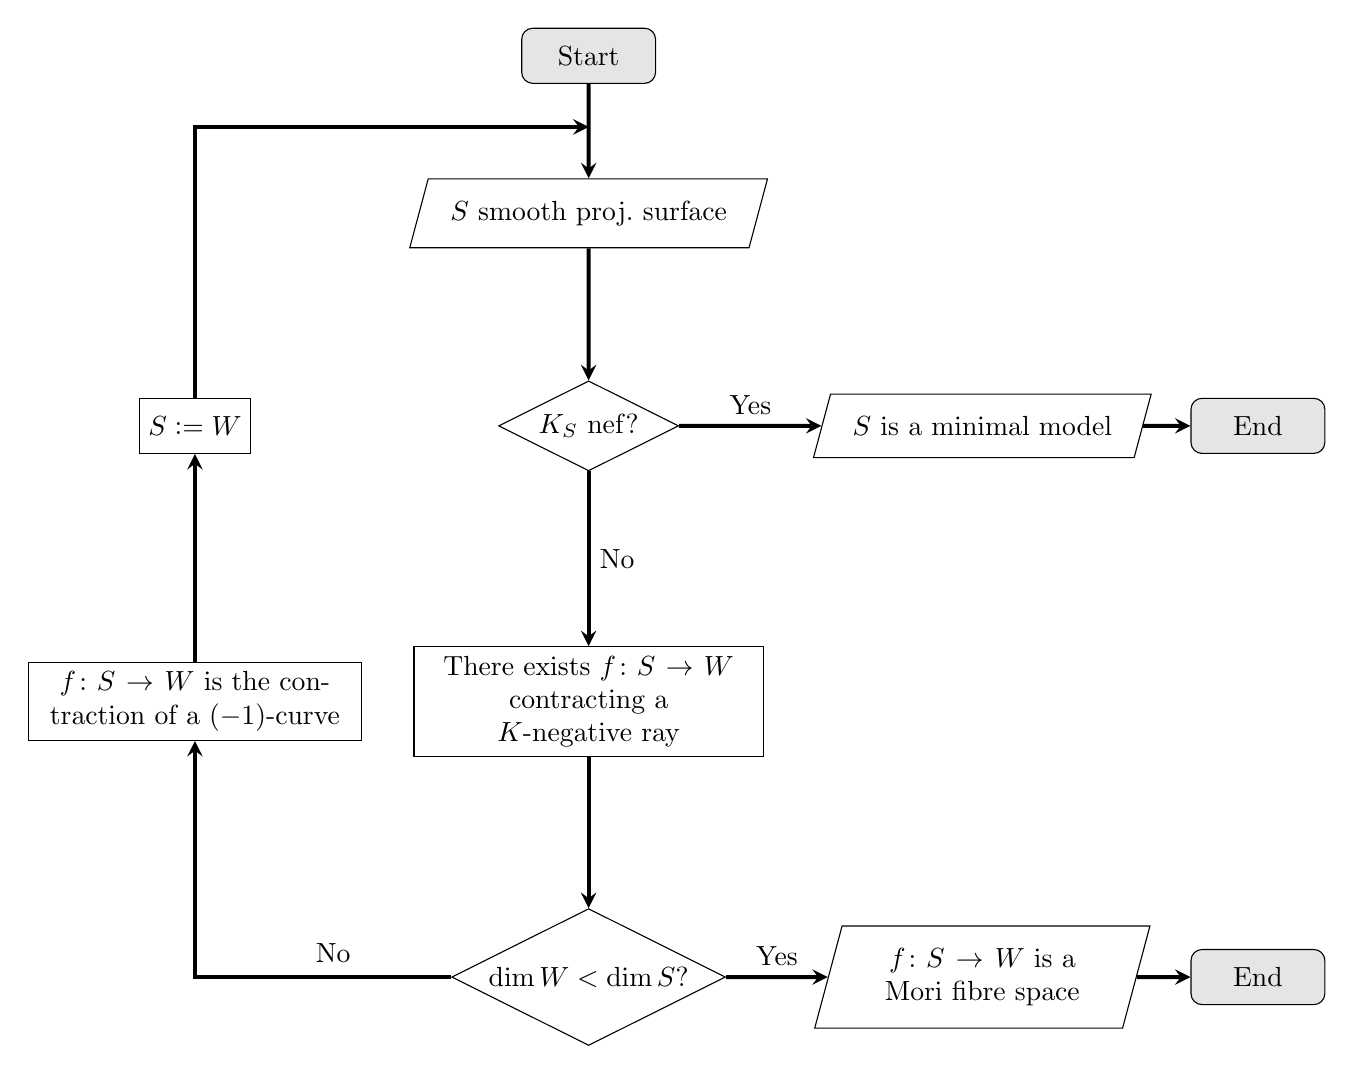
\begin{tikzpicture}[node distance=2cm]
	%%%Nodes
	
	\node(start)[startstop]{Start};
	
	\node(input) [io, below of=start] {$S$ smooth proj.\ surface};
	
	\node(Ks nef?)[decision, below of=input,yshift=-0.7cm] {$K_S$ nef?};
	
	\node(min model) [io, right of=Ks nef?,xshift=3cm] {$S$ is a minimal model};
	
	\node(end1)[startstop, right of=min model,xshift=1.5cm]{End};
	
	\node(cone thm) [process, below of=Ks nef?, yshift=-1.5cm, text width=4.2cm] {There exists $f\colon S \to W$ contracting a $K$-negative ray};
	
	\node(dimW) [decision, below of=cone thm, yshift=-1.5cm] {$\dim W < \dim S$?};
	
	\node(Mfs) [io, right of=dimW,xshift=3cm,text width=3cm] {$f \colon S \to W$ is a Mori fibre space};
	
	\node(end2)[startstop, right of=Mfs,xshift=1.5cm]{End};
	
	\node(blow down) [process, left of=cone thm, text width=4cm,xshift=-3cm]{$f\colon S\to W$ is the contraction of a $(-1)$-curve};
	
	\node(S=W) [process, left of=Ks nef?, xshift=-3cm] {$S\defeq W$};
	
	%%%Arrows
	\draw [arrow] (start) -- (input);
	\draw [arrow] (input) -- (Ks nef?);
	\draw [arrow] (Ks nef?) -- node[anchor=south] {Yes}(min model);
	\draw [arrow] (min model) -- (end1);
	\draw [arrow] (Ks nef?) -- node[anchor=west] {No}(cone thm);
	\draw [arrow] (cone thm) -- (dimW);
	\draw [arrow] (dimW) --node[anchor=south] {Yes} (Mfs);
	\draw [arrow] (Mfs) -- (end2);
	\draw [arrow] (dimW) -|node[at start,xshift=-1.5cm, yshift=0.3cm]{No} (blow down);
	\draw [arrow] (blow down) -- (S=W);
	\draw [arrow] (S=W) |- ($(start.north)!0.45!(input.south)$);
\end{tikzpicture}
}
\end{center}

Note that, by Remark \ref{rem:contractions}\eqref{it:cotractions2}, this algorithm indeed terminates.

\subsection{Dichotomy and MMP for uniruled surfaces}


\begin{theorem}[Easy Dichotomy Theorem]
	Let $S$ be a smooth surface.
	Then the end result of an MMP starting from $S$ is a Mori fiber space if and only if there exists a nonempty open neighbourhood $U\subset S$ such that: for every $p\in U$ there exists an irreducible curve $p\in C$ so that $K_S\cdot C <0$.
\end{theorem}

\begin{proof}
	Assume that the end result of an MMP is a Mori fiber space $\phi \colon T \to B$.
	Then $f\colon S \to T$ is a composition of contractions of $(-1)$-curves.
	We then have the ramification formula
	\[
	K_S = f^*K_T + R,
	\]
	where $R$ is an effective divisor supported on curves contracted by $f$.
	
	If $B$ is a curve, choose $U = (\phi\circ f)^{-1}(B \setminus \phi\circ f(R))$.
	For any $p \in U$ let $C$ be the curve $(\phi\circ f)^{-1}(\phi\circ f(p))$.
	Then
	\[
	K_S \cdot C = (f^*K_T + R)\cdot C = K_T\cdot f_*C = K_T \cdot \phi^{-1}(\phi\circ f(p)) < 0,
	\]
	where the last inequality comes from the fact that $\phi$ contracts only $K_T$-negative curves.
	
	If $B$ is a point , choose $U = S \setminus R$.
	Note that $f(R)$ is a finite number of points.
	For any $p \in U$ choose a curve $C \subset T$ passing though $f(p)$ but not $f(R)$\footnote{convince yourselves that this is possible}. 
	Then again we may calculate that $K_S \cdot f^{-1}C < 0$.
	
	Now assume that there exists such $U \subset S$ but some MMP on $S$ ends with a minimal model $f\colon S \to T$.
	Write again the ramification formula
	\[
	K_S = f^*K_T + R;
	\]
	choose a point $p \in U \setminus R$ and a curve $C$ containing $p$ with $K_S \cdot C < 0$.
	Note that since $p \in C$ and $p\not\in R$, $C \not\subset R$ and so $R \cdot C \geq 0$.
	We then have
	\[
	0>K_S\cdot C = (f^*K_T + R)\cdot C = K_Tf_*C + R\cdot C \geq  K_Tf_*C,
	\]
	which is a contradiction, since $K_T$ is nef.
\end{proof}

\begin{corollary}
	If the result of \emph{some} MMP is a Mori fiber space/minimal model, then the result of \emph{every} MMP is a Mori fiber space/minimal model.
\end{corollary}

\begin{definition}\label{def:(uni)ruled}
	A variety $X$ of dimension $n$ is called \textbf{ruled/uniruled} if there exists a birational/generically finite rational map
	\[
	W \times \PP^1 \rmap X,
	\]
	where $W$ is a variety of dimension $n-1$.
\end{definition}

\begin{remark}
	We can always assume that $W$ in Definition \ref{def:(uni)ruled} is smooth, simply by considering the composition $\widehat{W}\times \PP^1 \to W \times \PP^1 \rmap X$, where $\widehat{W} \to W$ is a resolution of singularities.
\end{remark}


\begin{proposition}
	Let $S$ be a uniruled surface.
	Then, for a general $p\in S$, there exists a rational curve $C$ so that $K_S \cdot C < 0$.
	
	In particular the result of any MMP from $S$ is a Mori fiber space.
\end{proposition}

\begin{proof}
	Since $S$ is uniruled there exists a generically finite rational map $C \times \PP^1 \rmap S$, where $C$ is a smooth curve.
	By Proposition \ref{prop:resolution} we have a diagram
	\[
	\xymatrix@R=.5cm@C=.5cm{
		&W \ar[ld]_s \ar[rd]^r \\
	C \times \PP^1 \ar@{-->}[rr] && S 
	}
	\]
	where $s$ is a composition of blowups and $r$ is a generically finite morphism.
	
	Denote by $\pi_1$ and $\pi_2$ the projection to the two factors of $C \times \PP^1$	and, for a point $x \in C$, denote by $F_x$ the fiber $\pi_1^{-1}(x)$.
	Then $K_{C \times \PP^1} = \pi_1^*K_X + \pi_2^*\OO_{\PP^1}(-2)$ and so
	\[
	K_{C \times \PP^1} \cdot F_x = -2.
	\]
	The ramification formulas for $s$ and $r$ give
	\[
	K_W = s^*(K_{C \times \PP^1}) + R_s \, \text{ and } \, K_W = r^*K_S + E_r + R_r,
	\]
	where $E_r$ is a divisor contracted by $r$.
	Let $q \in W \setminus (R_s \cup E_r)$, $F_x$ a fiber containing $s(q)$ and denote by $\widehat{F}_x = s^{-1}F_x$.
	Then 
	\[
	K_W \cdot \widehat{F}_x = K_{C \times \PP^1}\cdot F_x + R_s \cdot \widehat{F}_x = -2
	\]
	and 
	\[
	\deg(r|_{\widehat{F}_x})K_S\cdot r(\widehat{F}_x) = K_S\cdot r_*\widehat{F}_x = r^*K_S \cdot \widehat{F}_x = (K_W - E_r - R_r)\cdot \widehat{F}_x \leq -2,
	\]
	which implies that $K_S \cdot r(\widehat{F}_x) < 0$.
	Moreover, since $r|_{\widehat{F}_x}$ is finite and $\widehat{F}_x \isom \PP^1$, $r(\widehat{F}_x) \isom \PP^1$.
\end{proof}

Later, in Theorem \ref{thm:Mfs}, we will see that Mori fiber spaces in dimension $2$ (and therefore varieties birational to Mori fiber spaces) are ruled.
In particular, \emph{in dimension $2$}, a variety is unirational if and only if it is ruled.
This is very not true in higher dimensions with the fisrt counterexample given by Iskovskikh and Manin \cite{Luroth}, in dimension $3$.

\subsection{Uniqueness of Minimal Models}

\begin{proposition}[{\emph{Minimality} of minimal models}]\label{prop:minimality}
	Let $S$ be a minimal model and $T$ a smooth surface.
	Then any birational map $f\colon T \rmap S$ is a morphism.
\end{proposition}

\begin{proof}
	By Proposition \ref{prop:resolution} we have a diagram
	\[
	\xymatrix@R=.5cm@C=.5cm{
		& W \ar[ld]_r \ar[rd]^s\\
		T \ar@{-->}[rr]^f && S,
	}
	\]
	where $r$ is a composition of blowups.
	Let $E_r$ be a $(-1)$-curve contracted by $r$.
	Writing the ramification formula for $s$ and intersecting with $E_r$ we get
	\[
	-1 = K_W\cdot E_r = \left(s^*K_S + R_s\right)\cdot E_r = K_S\cdot s_*E_r + R_s\cdot E_r.
	\]
	Since $K_S$ is nef, this is only possible if $R_s\cdot E_r < 0$, i.e.\ $E_r \subset R_s$ and so $E_r$ is contracted by $s$.
	By Proposition \ref{prop:rigidity} both $r$ and $s$ factor thought the contraction $W \to W_1$ of $E_r$
	\[
	\xymatrix@R=.3cm@C=.5cm{
	&W \ar[d] \ar@/_1pc/[ldd]_r \ar@/^1pc/[rdd]^s\\
	&W_1 \ar[ld]_{r_1} \ar[rd]^{s_1}\\
	T \ar@{-->}[rr]^f && S.
	}
	\]
	We may repeat this process until we finally show that $s$ contracts all curves contracted by $r$, which shows that $s$ factors $r$, i.e. $f$ is a morphism. 
\end{proof}

Proposition \ref{prop:minimality} justifies the name \emph{minimal} model in the following sense:
consider the partial ordered set of all smooth varieties in a birational equivalence class (up to isomorphism) with the ordering
\[
	T_2 \succeq T_1 \, \iff \, \text{ there exists a birational contraction } T_2 \to T_1; 
\]
let $S$ be a minimal model and suppose that $S \succeq T$;
then there exist a contraction $f\colon S \to T$;
by Proposition \ref{prop:minimality} $f^{-1}$ is also a morphism, i.e.\ $S \isom T$.


\begin{corollary}\label{cor:uniqueness}
	Let $S$, $T$ be minimal models.
	Then any birational map between them is an isomorphism.	
	In particular, minimal models are unique in their birational equivalence classes.
\end{corollary}

\section{Mori fiber spaces and the Sarkisov program}

\subsection{Classification of Mori fiber spaces in dimension $2$}

\begin{definition}
	A morphism $f\colon S \to C$ from a smooth surface $S$ to a smooth curve $C$ is called a \textbf{$\PP^1$-bundle} if for every point $p \in C$ there exists a neighbourhood $p \in U \subset C$ and a commutative diagram
	\[
	\xymatrix@R=.5cm@C=.5cm{
	f^{-1}(U) \ar[r]^{\sim} \ar[d]_f & U\times \PP^1 \ar[d]^{p_1}\\
	U \ar@{}[r]^(.25){}="a"^(.75){}="b" \ar@{=} "a";"b"& U.
	}
	\]
\end{definition}

\begin{theorem}\label{thm:Mfs}
	Let $f\colon S \to B$ be a Mori fibre space in dimension $2$.
	Then either
	\begin{itemize}
		\item $B$ is a smooth curve and $f\colon S \to B$ is a $\PP^1$-bundle or
		\item $S = \PP^2$, $W = pt$ and $f$ is the structure morphism.
	\end{itemize}
	
	Furthermore two $\PP^1$-bundles $f_1\colon S_1 \to C_1$ and $f_2\colon S_2 \to C_2$ are birational \emph{if and only if} $C_1 \isom C_2$.
\end{theorem}
\begin{center}
\begin{minipage}{.8\textwidth}
	\underline{Reminder - \emph{the exponential sequence and $\Pic(X)$}}: 
	for a variety over the complex numbers we have the \emph{exponential} exact sequence
	\[
	0 \to \ZZ \to \OO_X \to \OO_X^* \to 0,
	\]
	where $\OO_X \to \OO_X^*$ is locally given by $s \mapsto e^{s}$, with kernel the sheaf of locally constant functions with values in $2\pi i\ZZ$.
	This induces the corresponding long exact sequence in cohomology in the \emph{analytic category}.
	
	Moreover we have a natural identification of $\Pic(X)$ with $H^1(S,\OO_X^*)$:
	indeed a divisor $D \in \Pic(X)$ is a collection $\{(U_i,f_i)\}_{i\in I}$ of open subsets $U_i$ of $S$ with local equations $f_i$;
	the glueing data for the $f_i$ is the same data as a Cech cocycle of $\OO_X^*$. 
\end{minipage}
\end{center}

\begin{proof}
	We will take cases based on the dimension of the base $B$.
	
	\noindent\fbox{Case: $\dim(B) = 1$}\label{case:dimB1}
	
	Denote by $F = F_b$ the fiber $f^{-1}(b)$, for $b\in B$.
	Note that $F^2= 0$ and $K_S\cdot F < 0$ thus, by the \emph{arithmetic genus formula} (see Exercise \ref{exer:-1curveIsKNegative}), $F$ is a rational curve.
	
	We want to show that there is a neighbourhood $b\in U \subset B$ so that $f^{-1}(U) \isom U\times \PP^1$.
	Note that, by looking at the projection $U\times \PP^1 \to \PP^1$, we get infinite sections of $f^{-1}(U) \to U$.
	We begin by finding these sections.	
	
	$K_S$ is negative against all fibers of $f$, which are infinitely many;
	this implies that $K_S$ cannot be effective, and by Serre duality we get
	\[
	H^2(S,\OO_S) = H^0(S,\OO_S(K_S)) = 0.
	\]
	Therefore the cohomology sequence induced by the exponential sequence gives
	\[
	\cdots \to \Pic(S) \isom H^1(S,\OO_S^*) \overset{\eta}{\longrightarrow} H^2(S,\ZZ) \to H^2(S,\OO_S) = 0.
	\]
	Viewing $F$ as a cycle in $H_2(S,\ZZ)$, Poincar{\'e} duality and unimodularity of the cup product implies that there exists a class $z \in H^2(S,\ZZ)$ so that $z \cdot F = 1$.
	Using the fact that $\eta$ is surjective we find a divisor $D \in \Pic(S)$ so that $\eta(D) = z$, i.e.\ $D \cdot F = 1$.
	
	With some work one can show that, for $r \gg 0$, the divisor $D+rF$ has sections and the restriction
	\[
	H^0(S,\OO_S(D+rF)) \overset{\text{res}}{\longrightarrow} H^0(F,\OO_F(D+rF)) \isom H^0(\PP^1,\OO_{\PP^1}(1))
	\]
	is surjective.
	Choose lift a basis of $H^0(\PP^1,\OO_{\PP^1}(1))$ to a linear system $V \leq H^0(S,\OO_S(D+rF))$ and choose $p\in U\subset B$ so that $V$ has no base points on $f^{-1}(U)$.
	We then get a commutative diagram
	\[
	\xymatrix@R=.5cm@C=.3cm{
	f^{-1}(U) \ar[rr]^{\phi_{V}\times f} \ar[dr]_f && \PP^1 \times U \ar[ld]^{p_2}\\
	&U.
	}
	\]
	
	As for the furthermore part, if $C_1 \isom C_2 \isom C$ then $S_1$ and $S_2$ both contain open subsets isomorphic to $C \times U$ and so they are birational.
	Assume now that $S_1$ is birational to $S_2$ and let $\chi \colon S_1 \to S_2$ be a birational map.
	If both $C_1$ and $C_2$ are rational then we are done.
	So, without loss of generality, assume that $g(C_2) \geq 1$.
	Then $\chi$ maps fibers to fibers:
	indeed, choose a fiber $F_1$ away from any base points of $\chi$ and suppose that $\chi(F_1)$ is not a fiber;
	then $f_2\circ \chi\colon F_1 \to C_2$ gives a finite morphism, which is impossible since $g(F_1) < g(C_2)$.
	
	We will now show that $\chi$ maps sections to sections too.
	Choose $U_i \subset C_i$ open trivializing subsets for $S_i \to C_i$, i.e.\ $f_i^{-1}(U_i) \isom U_i \times \PP^1$. 
	Then, since $\chi|_{U_1\times \PP^1}$ preserves intersection numbers and maps fibers to fibers, the image of a section $U_1 \times 0$ is a section $U_2 \times p$.
	Thus $U_1 \isom U_2$ via
	\[
	U_1 \isom U_1 \times 0 \overset{\chi}{\longrightarrow} U_2 \times p \isom U_2
	\]
	and so $C_1$ is birational to $C_2$.
	Since $C_i$ are smooth, they are isomorphic.	
	
	\noindent\fbox{Case: $\dim(B) = 0$}
	
	In this case $\rho(S) = 1$ and so $\NE(S) = \NEb(S)$.
	Moreover $-K_S$ is positive against all curves on $S$ and thus ample by Theorem \ref{thm:NM}.
	Let $H$ be an ample generator of $\Pic(S)$ and $r$ an integer so that $-K_S = rH$.
	Moreover, by Theorem \ref{thm:SerreKodairaVanishing} for $A = -K_S$ and $A = (1+r)H$ we get
	\[
	H^1(S,\OO_S) = H^2(S,\OO_S) = 0 \, \text{ and } \, H^1(S,\OO_S(H)) = H^2(S,\OO_S(H)) = 0.
	\]
	The exponential sequence then yields
	\[
	\Pic(S) = H^2(S,\ZZ)
	\]
	and, by Poincar{\'e} duality and the unimodularity of the cup product, $H^2 = 1$.
	Moreover $\chi(\OO_S) = h^0(S,\OO_S) = 1$ and the Riemann-Roch gives
	\[
	h^0(S,\OO_S(H)) = \frac{(H-K_S)H}{2} = \chi(\OO_S) = \frac{1+r}{2} + 1 \geq 2.
	\]
	Thus, there exists a (necessarily irreducible and reduced) curve $C \in H^0(S,\OO_S(H))$.
	The arithmetic genus formula (see Exercise \ref{exer:-1curveIsKNegative}) yields
	\[
	0 \leq h^1(D,\OO_D) = \frac{(H+K_S)H}{2} + 1 = \frac{1-r}{2} + 1 \leq 1,
	\]
	i.e.\ either $r = 1$ or $r = 3$.
	
	\noindent\fbox{Subcase: $r = 3$}\label{subcase:index3}
	In this case $h^0(S,\OO_S(H)) =3$, $D\isom \PP^1$ and the exact sequence
	\[
	\cdots \to H^0(S,\OO_S(H)) \to H^0(D,\OO_D(H)) \isom H^0(\PP^1,\OO_{\PP^1}(1)) \to H^1(S,\OO_S) = 0
	\]
	shows that the complete linear system $H^0(S,\OO_S(H))$ has no base points.
	It therefore gives a finite morphism $\phi_H\colon S \to \PP^2$. Finally
	\[
	1 = H^2 = \deg(\phi_H)\OO_{\PP_2}(1)^2 = \deg(\phi_H),
	\]
	so $\phi_H$ is an isomorphism.
	
	\noindent\fbox{Subcase: $r = 1$}
	In this case $h^0(S,\OO_S(H)) =2$ and so $H^0(S,\OO_S(H))$ must have a (unique) base point $p$:
	otherwise we would get a surjective morphism $S \to \PP^1$ which is impossible since $\rho(S) = 1$.	
	Moreover $D$ is an elliptic curve.
	However $\OO_D(H) = \OO_D(p)$ which is effective, and so the exact sequence
	\[
	\cdots \to H^0(S,\OO_S(H)) \to H^0(D,\OO_D(p)) \to H^1(S,\OO_S) = 0
	\]
	shows again that $H$ has no base points on $D$, a contradiction!
	
	
	\begin{comment}
	In this case $h^0(S,\OO_S(H)) =2$ and so $H^0(S,\OO_S(H))$ must have a (unique) base point $p$:
	otherwise we would get a surjective morphism $S \to \PP^1$ which is impossible since $\rho(S) = 1$.	
	
	We want to get a contradiction by proving that $H$ is base point free.
	Ideally we would like to use an argument as in \hyperref[subcase:index3]{{\small \fbox{Subcase: $r=3$}}}; however we now have that, for a general $D \in H^0(S,\OO_S(H))$, $g(D) = 1$.
	Instead we will show that the linear system $H^0(S,\OO_S(H))$ is \emph{``locally isotrivial''}, i.e.\ general elements are isomorphic to each other;
	then we will use Exercise \ref{exer:bendAndBreak} to produce a (singular) rational element $D_0 \in H^0(S,\OO_S(H))$.
	
	Let $f\colon T \to S$ denote the blowup along $p$.
	The divisor $L_s = s\tilde{H} + E = sf^*H - (s-1)E$ is ample for any $s > 1$:
	it is clearly positive against any curve not contracted by $f$ by the pull-push formula (see Definition \ref{def:pull-push}), and $L_s \cdot E= 1$.
	Furthermore
	\[
	K_T = f^*K_S + E = f^*(-H) + E = -\tilde{H} - E + E = -\tilde{H}
	\]
	and so
	\[
	h^i(T,L_s) = h^i(T, K_T + L_{s-1}) \text{ and } h^i(T,L_s - \tilde{H}) = h^i(T,K_T + L_{s-2}) 
	\] 
	which vanish for $i=1,2$ and $s > 3$ by Theorem \ref{thm:SerreKodairaVanishing}.
	Thus by Riemann-Roch we get
	\[
	h^0(T,L_S) = \frac{(L_s + K_T)L_s)}{2} + 1 = s^2 - s +1 > 2
	\]
	and, for any $D \in |\tilde{H}|$ using the structure sequence for $D$, we get that the restriction map
	\[
	H^0(T,\OO_S(L)) \overset{\text{res}}{\longrightarrow} H^0(D,\OO_D(L)) \isom H^0(D,\OO_{D}(p))
	\]
	is surjective.
	This implies that $L$ has no base points in a neighbourhood of $D$, and as in \hyperref[case:dimB1]{{\small \fbox{Case: $\dim B = 1$}}} we conclude that $T$ has a neighbourhood isomorphic to $U \times D$. 
	
	Therefore, by Exercise \ref{exer:bendAndBreak}, there exists a (singular) rational curve $D_0 \in H^0(S,\OO_S(H))$.
	Since $H^2 = 1$ elements of $D \in H^0(S,\OO_S(H))$ cannot intersect $D_0$ at its singular locus, since there the local intersection multiplicity is at least $2$.
	Let $p \in D_0$ be a point of intersection with a section $D$ of $H$, then we get the exact sequence
	\[
	\cdots H^0(S,\OO_S(H)) \to H^0(D_0,\OO_{D_0}(H)) \isom H^0(D_0,\OO_{D_0}(p)) \to H^1(S,\OO_S) = 0.
	\]
	However $H^0(D_0,\OO_{D_0}(p))$ has sections that don't vanish at $p$;
	in particular the previous exact sequence shows that $H^0(S,\OO_S(H))$ has no base points, a contradiction.
	\end{comment}
\end{proof}

\begin{remark}\leavevmode	
	\begin{enumerate}
		\item In the last subcase, one can avoid working with elliptic curves and instead use a \emph{Bend-and-Break} argument to find a (singular) rational curve $D_0 \in H^0(S,\OO_S(H))$ (see Exercise \ref{exer:bendAndBreak}).
		\item In the same subcase we obtained a contradiction to $-K_S$ being base point free from the fact that $\rho(S) = 1$.
		There does exist a surface with the same numerics ($-K_S$ ample and $(-K_S)^2 = 1$) where everything else works as intended;
		However this surface has Picard rank $\rho(S) = 9$ (see Exercise \ref{exer:proj})
	\end{enumerate}
\end{remark}

\subsection{Some fundamental examples - low degree and Hirzebruch surfaces}\label{subsec:exaples}

\vspace{.3cm}

\begin{center}
	\begin{minipage}{.9\textwidth}\label{rem:adjunction}
		{\underline{Reminder - \emph{the adjunction formula}}}:
		Let $Y\subset X$ be smooth varieties, so that $\dim Y = \dim X - 1$.
		Then $K_Y = (K_X + Y)|_Y$.
	\end{minipage}
\end{center}

\vspace{.3cm}

\begin{lemma}
	Let $S\subset \PP^3$ be a smooth surface.
	Then $-K_S$ is ample if and only if $\deg(S) \leq 3$.
\end{lemma}

\begin{proof}
	By the adjunction formula $-K_S = (4-\deg(S))H|_S$.
	Moreover $H|_S$ is ample and so we conclude.
\end{proof}

\noindent\href{https://s-zikas.github.io/site/pics/italianSchool.jpg}{{\underline{\emph{Quadric surfaces:}}}} we will show that smooth quadric surfaces are all isomorphic to $\PP^1 \times \PP^1$.

\begin{lemma}\label{lem:coneP1P1}
	The cone $\NE(\PP^1 \times \PP^1)$  is generated by the classes of fibers of the two fibrations $\PP^1 \times \PP^1 \to \PP^1$.
\end{lemma}

\begin{proof}
	First note that $\rho(\PP^1 \times \PP^1) = 2$:
	indeed, let $(u_0:u_1), (v_0:v_1)$ be the coordinates and let $C = \{f_{i,j} = 0\}$ be a curve, where $f_{i,j}$ is a curve of bidegree $(i,j)$;
	then $f \defeq \frac{f_{i.j}}{u_0^iv_0^j}$ is a well-defined rational function with $\divv(f) = C - iF_1 - jF_2$, where $F_1$ and $F_2$ are the classes of fibers of the the two projections.
	By Proposition \ref{prop:rigidity} $F_1$ and $F_2$ span extremal rays.
	Since $\rho(\PP^1 \times \PP^1) = 2$, $\NE(\PP^1 \times \PP^1)$ has at most $2$ extremal rays and so we conclude.
\end{proof}

\begin{remark}
	The first claim is very not true for arbitrary products:
	Let $C$ be an elliptic curve, $S = C \times C$ and $\Delta$ be the diagonal;
	$K_S = p_1^*K_C \otimes p_2^*K_C = 0$ and the arithmetic genus formula yields
	\[
	1 = p_a(\Delta) = \frac{\Delta^2}{2} + 1 \implies \Delta^2 = 0;
	\]
	assuming that $\Delta = a_1F_1 + a_2F_2$ and intersecting with $F_1$ and $F_2$ we get that $a_1 = a_2 = 1$;
	but then $\Delta^2 = 2$, a contradiction.
\end{remark}

\begin{lemma}\label{lem:imageOfP1P1}
	Let $D$ be a divisor of bidegree $(1,1)$ in $\PP^1 \times \PP^1$.
	Then $D$ is very ample and, up to a choice of basis, its complete linear system gives an isomorphism
	\[
	\PP^1 \times \PP^1 \to \{x_0x_3 - x_1x_2 = 0\} \subset \PP^3.
	\]
\end{lemma}

\begin{proof}
	We have the basis
	\[
	H^0(\PP^1 \times \PP^1,\OO_{\PP^1 \times \PP^1}(1,1)) = \langle u_0v_0, u_0v_1, u_1v_0, u_1v_1 \rangle.
	\]
	We may check that the corresponding map has no base points and thus gives a morphism to $\PP^3$, whose image is $\{x_0x_3 - x_1x_2 = 0\}$.
	This map is clearly generically one-to-one.
	Moreover $D \cdot F_i =1$ and so, by Lemma \ref{lem:coneP1P1} and Theorem \ref{thm:NM}, it is ample and therefore contracts no curves.
	We conclude it's an isomorphism by Proposition \ref{prop:rigidity}.
\end{proof}



\begin{proposition}\label{prop:quadricP1P1}
	A smooth quadric surface $S \subset \PP^3$ is isomorphic to $\PP^1 \times \PP^1$.
\end{proposition}

\begin{proof}
	By Lemma \ref{lem:imageOfP1P1} it suffices to show that, given a smooth quadric $\{q = 0\}$ with
	\[
	q = \sum q_{i,j}x_ix_j,
	\]
	we can change coordinates to $x_0x_3 - x_1x_2$.
	Note that $q$ can be identified with a quadratic form $Q$ via
	\[
	2q(x_0,x_1,x_2,x_3) = (x_0,x_1,x_2,x_3)
	\left(
	\begin{array}{cccc}
		2f_{0,0} & f_{0,1} & f_{0,2} & f_{0,3}\\
		f_{1,0} & 2f_{1,1} & f_{1,2} & f_{1,3}\\
		f_{2,0} & f_{2,1} & 2f_{2,2} & f_{2,3}\\
		f_{3,0} & f_{3,1} & f_{3,2} & 2f_{3,3}
	\end{array}
	\right)
	\begin{pmatrix}
		x_0\\
		x_1\\
		x_2\\
		x_3
	\end{pmatrix}.
	\]
	The action of a matrix $M \in \GL_4$ to $q$ corresponds to acting on $Q$ via $M Q M^t$.
	Acting with suitable matrices we can always diagonalize $Q$, i.e.\ change coordinates so that
	\[
	q \mapsto q'= x_0^2 + x_1^2 + x_2^2 + x_3^2 = (x_0 + ix_1)(x_0 - ix_1) + (x_2 + ix_3)(x_2 - ix_3).
	\]
	Acting once more by the inverse of the matrix
	\[
	M = 
	\left(
	\begin{array}{rrrr}
		1 & 0 & 0 & 1\\
		i & 0 & 0 & -i\\
		0 & 1 & 1 & 0\\
		0 & i &-i & 0
	\end{array}
	\right)
	\]
	we get to the required form.
\end{proof}

\noindent\underline{\emph{Cubic surfaces:}} we will show that smooth cubic surfaces are isomorphic to $\PP^2$ blown up at $6$ points in general position, that is no $3$ on a line and no $6$ on a conic.
 
In what follows $S$ will denote the blowup of $\PP^2$ along $6$ points $p_1,\dots, p_6$ in general position, with exceptional divisors $E_1, \dots, E_6$.
Then, by Proposition \ref{prop:blp}, $\Pic(S) = \langle L, E_1, \dots, E_6 \rangle$, where $L$ denotes the pullback of the class of a line in $\PP^2$.

\begin{lemma}\label{lem:antiCanAmple}
	The anti-canonical divisor $-K_S$ is ample.
	Moreover there exists exactly $27$ irreducible curves with the property $-K_S \cdot C = 1$.
\end{lemma}

\begin{proof}
	Denote by $l_{i,j}$ the strict transform of the unique line thought the points $p_i,p_j$ and by $c_i$ the strict transform of the unique conic thought the points $p_1,\dots,\hat{p_i},\dots p_6$.	
	We then have
	\[
	-K_S = 3L - E_1 - \ldots - E_6
	\]
	and we may calculate that
	\[
	-K_S\cdot E_i = 1, \quad -K_S\cdot l_{i,j} = 1, \quad -K_S\cdot c_i = 1;
	\]
	these give exactly $6 + \binom{6}{2} + 6 = 27$ classes that are $1$ against $-K_S$.
	
	Let $C$ be an irreducible curve, not one of the above, such that $-K_S\cdot C \leq 1$.
	By Proposition \ref{prop:blp} $C  \sim dL - m_1E_1 - \ldots - m_6E_6$ with $d > 0$ and $m_i \geq 0$.
	Without loss of generality assume that $m_1 \geq m_2 \geq \ldots \geq m_6$.
	Since $C\cdot c_6 \geq 0$ and $C\cdot l_{1,6}\geq 0$,
	\begin{gather*}
		 c_6  = 2d - m_1 - \ldots - m_5 \, \text{ and } \, 0\leq  d - m_1 - m_6\\\
		\implies  3d - m_1 - \ldots - m_6 \geq m_1 \implies -K_S\cdot C \geq m_1.
	\end{gather*}
	If $-K_S\cdot C = 0$ then $m_1 = \ldots = m_6 =0$ and then $d=0$, a contradiction.
	If $-K_S\cdot C = 1$ then $m_i \leq 1$ which gives $d = 1$ or $2$ and in turn implies that $C = l_{i,j}$ or $C = c_i$ for some $1 \leq i,j \leq 6$, again a contradiction.
\end{proof}

\begin{proposition}\label{prop:cubicEmbedding}
	The anti-canonical divisor $-K_S$ is very ample and defines an embedding $S \to T \subset \PP^3$, where $T$ is a smooth cubic surface.
\end{proposition}

\begin{proof}
	Since $-K_S$ is ample by Lemma \ref{lem:antiCanAmple}, by Theorem \ref{thm:SerreKodairaVanishing} applied for $A = -K_S$ and $A = -2K_S$ respectively, we get $h^1(S,\OO_S) = h^2(S,\OO_S) = 0$ and $h^1(S,-K_S) = h^2(S,-K_S) = 0$.
	We may compute that $(-K_S)^2 = 3$ and so Riemann-Roch gives
	\[
	h^0(S,-K_S) = (-K_S)^2 + 1 = 4.
	\]
	
	We first show that $-K_S$ is bpf.
	Let $p$ be a base point of $-K_S$ and let $E \in |-K_S|$ be an irreducible curve.
	We then have
	\begin{equation}\label{eq:resCubic}\tag{res}
	\dots \to H^0(S,-K_S) \to H^0(E,-K_S|_E) \to H^1(S,\OO_S) = 0
	\end{equation}
	Since $-K_S|_E$ is effective, we may lift constant sections to show that $-K_S$ has no base points on $E$, and therefore no base points at all.
	
	We now show that $-K_S$ is very ample.
	Let $f \colon S \to T \subset \PP^3$ be the morphism associated to $-K_S$ and let $S \to S' \to T$ be its Stein factorization, i.e.\ $S \to S'$ has connected fibers and $S'\to T$ is finite.
	Since $-K_S$ is ample, it cannot contract any curves, i.e.\ $S \isom S'$.
	Assume that $f\colon S \to T$ is finite.
	Since $-K_S$ is base point free then a general $E \in |-K_S|$ is smooth.
	Choose such $E$ so that it's not contained in the ramification locus of $S \to T$.
	$E$ is an elliptic curve and $-K_S|_E$ is a divisor of degree $3$.
	By Riemann-Roch on $E$ we get
	\[
	h^0(E,-K_S|_E - p) = h^0(E,-K_S|_E) - 1 \, \text{ and } \, h^0(E,-K_S|_E - p - q) =h^0(E,-K_S|_E) - 2
	\]
	and so $-K_S|_E$ is very ample.
	Moreover \eqref{eq:resCubic} shows that $f|_E$ coincides with the morphism given by $-K_S|_E$ and is thus an isomorphism, i.e.\ $f$ is an isomorphism.
	
	Finally we have
	\[
	\deg(T) = T\cdot \OO_{\PP^3}(1)^2 = (\OO_{\PP^3}(1)|_T)^2 = \OO_{T}(1)^2 = f^*(\OO_{T}(1))^2 = -K_S^2 = 3. 
	\]
\end{proof}



\begin{remark}[{\href{https://s-zikas.github.io/site/pics/27lines.png}{27 lines}}]\label{rem:27lines}
	With respect to the embedding given by $-K_S$, lines are curves with $-K_S \cdot C = 1$.
	Lemma \ref{lem:antiCanAmple} shows that there are precisely $27$ lines in $T$.
\end{remark}



\begin{proposition}\label{prop:cubic}
	Let $T \subset \PP^3$ be a smooth cubic surface.
	Then
	\begin{enumerate}
		\item\label{it:cubic1} $T$ contains a line;
		\item\label{it:cubic2} if $l$ is a line in $T$, then the projection $T \to \PP^1$ has $r$ singular fibers, with $2\leq r\leq 5$;
		\item\label{it:cubic3} $T$ contains at least a configuration of $r+1$ skew lines.
	\end{enumerate}
\end{proposition}

\begin{proof}
	Consider the correspondence
	\[
	\mathcal{X} = \big\{(T,l) \in \PP\left(|\OO_{\PP^3}(3)|\right) \times G(2,4) \,\big|\, l\subset T \big\}
	\]
	with the two projections $p_1$ and $p_2$.
	
	We will first study the second projection.
	First of all $p_2$ is surjective.
	Let $l$ be a line and, without loss of generality, $l = \{x_0 = x_1 = 0\}$.
	Then
	\[
	p_2^{-1}(l) = \{ f(x_0,x_1,x_2,x_3)x_0 + g(x_1,x_2,x_3)x_1 = 0 \}
	\]
	which has dimension $\binom{3+2}{3} + \binom{2+2}{2} -1 = 15$.
	Thus $\dim(\mathcal{X}) = 15 + 4 = 19$.
	
	We only need to show that the first projection is surjective.
	Since $\dim(\mathcal{X}) = 19 = \dim\PP\left(|\OO_{\PP^3}(3)|\right)$, $p_1$ can only fail to be surjective if all the fibers have positive dimension.
	By lower semi-continuity of the dimension of the fibers, it suffices to find a cubic surface with only finitely lines.
	For that we may choose a cubic as in Proposition \ref{prop:cubicEmbedding} and conclude by Remark \ref{rem:27lines}.
	This is \eqref{it:cubic1}.
	
	Let $l \subset T$ be one of the lines in \eqref{it:cubic1} and consider the projection from $l$
	\[
	\begin{array}{ccc}
		\PP^3 &\rmap & \PP^1\\
		(x_0:\ldots:x_3) & \mapsto & (x_0:x_1).
	\end{array}
	\]
	This extends to a morphism $T \to \PP^1$.
	For a point $(\lambda_0:\lambda_1) \in \PP^1$ the fiber of $T \to \PP^1$ is residue of the intersection of the plane $\Pi_{\lambda_0,\lambda_1} \defeq \{\lambda_1 x_0 - \lambda_0 x_1 = 0\}$ with $T$.
	This is of the form
	\[\arraycolsep=-.5cm
	\begin{array}{ccccc}
		\alpha_{0,0}(\lambda_1,\lambda_2)x_2^2 & + & \alpha_{0,1}(\lambda_1,\lambda_2)x_2x_3 & + & \alpha_{1,1}(\lambda_1,\lambda_2)x_2^2 \,+\\
		&\beta_{0,2}(\lambda_1,\lambda_2)x_1x_2 &+& \beta_{1,2}(\lambda_1,\lambda_2)x_1x_3 \,+\\
		&&\gamma_{2,2}(\lambda_1,\lambda_2) x_1^2\, =0,
	\end{array}
	\]
	where $\alpha_{i,j}$, $\beta_{i,j}$ and $\gamma_{i,j}$ are linear, quadratic and cubic in $\lambda_1,\lambda_2$ respectively.
	This, up to multiplying by $2$, corresponds to the quadratic form
	\[
	Q(\lambda_1,\lambda_2) = 
	\left(
	\begin{array}{ccc}
		2\alpha_{0,0}(\lambda_1,\lambda_2) & \alpha_{0,1}(\lambda_1,\lambda_2) & \beta_{0,2}(\lambda_1,\lambda_2)\\
		\alpha_{0,1}(\lambda_1,\lambda_2) & 2\alpha_{1,1}(\lambda_1,\lambda_2) & \beta_{1,2}(\lambda_1,\lambda_2)\\
		\beta_{0,2}(\lambda_1,\lambda_2) & \beta_{1,2}(\lambda_1,\lambda_2) & 2\gamma_{2,2}(\lambda_1,\lambda_2)
	\end{array}
	\right)
	\]
	and is singular precisely when $Q$ drops rank or equivalently when $\det(Q) = 0$.
	This is a homogenous polynomial of degree $5$ in $\lambda_1,\lambda_2$ and thus will have between $1$ and $5$ distinct roots.
	Furthermore if $\det(Q) = 0$ has exactly one solution, up to a change of coordinates, we may assume that the singular fiber is  the intersection with the plane $\{x_0 - \lambda_0x_1 = 0\}$ and $\det(Q) = \lambda_0^5$.
	Imposing the corresponding conditions on the equation of $T$ we see that then either $T$ has a triple point or is double along $l$.
	Since we assume that $T$ is smooth, $\det(Q) = 0$ has between $2$ and $5$ distinct roots;
	this is \eqref{it:cubic2}.
	
	The singular fibers of \eqref{it:cubic2} correspond to triangles of coplanar lines
	\begin{gather*}
		\Delta_1 = \{l,l_{1,1},l_{1,2}\}, \, \dots, \, \Delta_r = \{l,l_{r,1},l_{r,2}\}.
	\end{gather*}
	Repeating the process by replacing $l$ with $\mu = l_{1,1}$ we get another set of triangles
	\[
		A_1 = \{\mu, \mu_{1,1}, \mu_{1,2}\}, \, \dots, \, A_k = \{\mu, \mu_{k,1}, \mu_{k,2}\}.
	\]
	Note that the line $\mu_{k,1}$ can intersect at most one of the $l_{i,1}, l_{i,2}$: otherwise it would intersect the corresponding plane in $2$ points;
	but then it would be contained in that plane, which is impossible since the unique plane containing $l,\mu$ also contains the unique third line $l_{1,2} = \mu_{1,2} \neq \mu_{k_1}$.
	Thus, up to possibly reordering, $\{\mu_{k,1}, l_{1,1}, \dots, l_{r,1}\}$ is a configuration of $r+1$ skew lines.
\end{proof}


\begin{corollary}\label{cor:cubics=blp6}
	Every smooth cubic surface is $T$ isomorphic to $\PP^2$ blown up at $6$ points in general position.
\end{corollary}

\begin{proof}
	We first prove that every line is a $(-1)$-curve.
	Indeed, let $l$ be a line, then
	\[
	K_T \cdot l = \OO_{T}(-1)\cdot l = \OO_{\PP^3}(-1) \cdot l = -1.
	\]
	Moreover $l\isom \PP^1$ and so, by the arithmetic genus formula, $l^2 = -1$.
	
	Proposition \ref{prop:cubic}\eqref{it:cubic2} implies that $\rho(T) = r+2$:
	indeed we choose a $(-1)$-curve in each fiber and contract them $T \to W \to \PP^1$;
	the end result will give us a $\PP^1$-bundle (see proof of Theorem \ref{thm:Mfs}), since all remaining fibers are smooth conics or lines and so
	\[
	\rho(T) = \rho(W) + r = r+2.
	\]
	
	By \ref{prop:cubic}\eqref{it:cubic3}, there exists a configuration of $r+1$ skew lines;
	contracting it $T \to W$ we get that $W$ is a Mori fiber space of Picard rank $1$, i.e.\ $W \isom \PP^2$ and $T$ is the blowup of $\PP^2$ along $r+1$ points, with $1 \leq r \leq 5$.
	Finally it suffices to notice that 
	\[
	3 = (-K_T)^2 = (-K_{\PP^2})^2 - (r+1) = 9 - r -1 \implies r=5.
	\]
\end{proof}


Finally we compute the cone of curves of a smooth cubic surface.

\begin{proposition}
	Let $S$ be a smooth cubic surface.
	Then $\NE(S)$ is a rational polyhedral cone spanned by the classes of the $27$ lines on $S$.
\end{proposition}


\begin{proof}
	Since $-K_S$ is ample, $K_S$ is negative against \emph{every} curve.
	By Theorem \ref{thm:contrK-neg} every extremal ray of $\NE(S)$ is contractible and, by Proposition \ref{prop:rigidity}, it suffices to find all contractions $S \to W$ with $\rho(S) - \rho(W) =1$.
	Again by Theorem \ref{thm:contrK-neg} these can only be contractions of $(-1)$-curves, i.e.\ all extremal rays are spanned by $(-1)$-curves.
	It suffices to notice that a curve is a $(-1)$-curve on $S$  if and only if it is a line:
	one direction was proved in Corollary \ref{cor:cubics=blp6};
	as for the inverse, if $C$ is a $(-1)$-curve, then by the arithmetic genus formula 
	\[
	1 = -K_S\cdot C = H|_S\cdot C;
	\]
	thus $C$ is a curve of degree $1$ in $\PP^3$, i.e.\ a line.
\end{proof}

\begin{remark}
	Singular cubic surfaces with only double points arise again as the blowup of $\PP^2$ at six points, but this time not in general position; this also includes infinitely near points.
	For a very comprehensive treatment of the subject see \cite[Chapter 9]{Dolgachev}.
\end{remark}


\noindent\underline{\emph{The many manifestations of Hirzebruch surfaces}}

\begin{definition}
	We define the \textbf{$\mathbf{n}$-th Hirzebruch surface} to be the surface
	\[
	\FF_n \defeq \left\{ (x_0:x_1:x_2),(u_0:u_1) \in \PP^2\times \PP^1 \, \middle| \, x_0u_1^n - x_1u_0^n = 0 \right\}.
	\]
	In particular, $\FF_1$ is the blowup of $\PP^2$ along a point and $\FF_0$ is isomorphic to $\PP^1 \times \PP^1$.
	
	Note that the projection to the second factor $p_2 \colon \FF_n \to \PP^1$ is a $\PP^1$-bundle.
\end{definition}

Hirzebruch surfaces come in many manifestations;
different ones allow for certain calculations to be carried out easier.

\vspace{.3cm}

\noindent\hypertarget{hirzGIT}{\underline{\emph{As GIT quotients:}}}
Consider $\CC^4$ with coordinates $(y_0,y_1,v_0,v_1)$ and the following linear action of $G \defeq (\CC^*)^2$ on  $U \defeq \CC^4 \setminus \big( \{y_0=y_1 =0\}\cup \{v_0= v_1 =0\} \big)$:
\[
\begin{array}{ccc}
	\rho_n\colon G \times U & \to & U\\
	(\lambda,\mu), (y_0,y_1,v_0,v_1) & \mapsto & (\lambda y_0,\mu^{-n}\lambda y_1,\mu v_0,\mu v_1).
\end{array}
\]
All points on $U$ are semi-stable with respect to $\rho_n$, that is for any $x\in U$, $0 \not\in \overline{G\cdot x}$;
this implies that the projective quotient $S_n \defeq \PP(U)//G$ exists.
Furthermore, all points are actually stable, i.e.\ they are semi-stable, their orbit $G\cdot x$ is closed and all stabilizers $G_x$ are finite;
thus the quotient $S_n$ is geometric.
One of the very desirable properties that this entails is that  subvarieties of $S_n$ are cut out by polynomials in $\kk[y_0,y_1,v_0,v_1]$ whose zero locus is invariant under the action of $G$ (see \cite{Brion} for an introduction to actions of algebraic groups, and more specifically Proposition 1.31).

A compact way to write this data is with the \emph{grading matrix}
\[
\begin{array}{c}	
	\hspace{4pt}
	\begin{array}{cccc}
		y_0 & y_1 & v_0 & 
		\hspace{-5pt}v_1 
	\end{array}\\
	\left(
	\begin{array}{rr|rr}
		1 & 1 & 0 & 0\\
		0 & -n & 1 & 1
	\end{array}	
	\right)
\end{array}
\]
where the vertical bar indicates the irrelevant ideal.

We then have an isomorphism
\[
\begin{array}{ccc}
	\FF_n & \to & S_n\\
	(x_0:x_1:x_2),(u_0:u_1) & \mapsto & 
	\left\{ 
	\begin{array}{cc}
		\left(x_0:\frac{x_1}{u_0^n} \,; u_0:u_1\right), & \text{ when } u_0 \neq 0 \\
		\left(x_0:\frac{x_2}{u_1^n} \,; u_0:u_1\right), & \text{ when } u_1 \neq 0
	\end{array}
	\right.\\
	(y_0:y_1u_0^n:y_1u_1^n),(v_0:v_1) & \mapsfrom & (y_0:y_1\,; v_0:v_1).
\end{array}
\]


\begin{proposition}\label{prop:intersectionFFn}
	Denote by $\sigma, \sigma_+ \subset \FF_n$ the curves $\{y_1 = 0\}$ and $\{y_0 = 0\}$ respectively and by $f = \{v_0=0\}$.
	Then $\Pic(\FF_n) = \langle \sigma_+, f \rangle$.
	
	Moreover the following relations determine intersection theory on $\FF_n$:
	\begin{enumerate}
		\item $\sigma \cdot f = \sigma_+\cdot f = 1$;
		\item $\sigma_+ \sim \sigma + nf$;
		\item $\sigma\cdot\sigma_+ = 0$, $f^2 =0$ and $\sigma^2 = -n$.
	\end{enumerate}
\end{proposition}

\begin{proof}
	Subvarieties in $\FF_n$ are cut out by polynomials in $y_0,y_1,v_0,v_1$ that are homogenous of some bidegree $(i,j)$ with repsect to $\rho_n$, i.e.\
	\[
	f((\lambda,\mu)(y_0,y_1,v_0,v_1)) = \lambda^i\mu^jf(y_0,y_1,v_0,v_1).
	\]
	For a curve $C$ cut out by a polynomial $f_{i,j}$ of bidegree $(i,j)$ we have
	\[
	C - (i\sigma  + j f) = \divv\left(\frac{f_{i,j}}{y_0^iv_0^j}\right),
	\]
	which shows that $\sigma_+$ and $f$ generate $\Pic(\FF_n)$.
	Note that $i,j$ don't necessarily have to be positive.
	
	The intersection between $\sigma$ and $\sigma_+$ with $f$ are the points $(1:0\,; 0:1)$ and $(0:1\, 0:1)$ respectively.
	Consider the rational functions $\frac{y_0}{y_1v_0^n}$ and $\frac{v_0}{v_1}$;
	their divisors give us linear equivalences $\sigma_+ \sim \sigma + n f$ and $f\sim f_1$, where $f_1 \defeq \{v_1=0\}$.
	Moreover $\sigma$, $\sigma_+$ and $f$, $f_1$ don't intersect set theoretically and
	\[
	\sigma^2 = \sigma (\sigma_+ - nf) = -n.
	\]
\end{proof}

\begin{proposition}\label{prop:contractionHirz}
	The complete linear system of $\sigma_+$ determines a contraction $\pi\colon \FF_n \to S$ with $\NE(\pi) = \RR_+\sigma$.
	In particular $\NE(\FF_n) = \RR_+ \sigma \oplus \RR_+f$.
\end{proposition}

\begin{proof}
	As always we want to find a nef divisor, zero against only $\sigma$ and show that it's base point free.
	By Proposition \ref{prop:intersectionFFn}, $\sigma_+\cdot \sigma = 0$.
	This is a divisor of bidegree $\left( \begin{smallmatrix}
		1 \\ 0
	\end{smallmatrix} \right)$ and so we may easily compute the basis
	\[
	H^0(\FF_n,\sigma_+) = \langle y_1v_0^n, y_1v_0^{n-1}v_1,\dots, y_1v_1^n, y_0 \rangle.
	\]
	We immediately see that $\sigma$ is bpf.
\end{proof}

Notice that the image $S\subset \PP^{n+1}$ is cut out by equations 
\[
\rank
\left(
\begin{array}{cccc}
	z_0 & z_1 & \dots & z_{n-1}\\
	z_1 & z_2 & \dots & z_n
\end{array}
\right) = 1.
\]
Note that these are only in the first $n+1$ factors;
moreover these equations are the ones defining the Veronesse embedding
\[
\begin{array}{ccc}
	\nu_n\colon \PP^1 & \to & \PP^{n}\\
	(t_0:t_1) & \mapsto & (t_0^n:t_0^{n-1}t_1:\ldots:t_1^n).
\end{array}
\]
This shows that $S$ is the cone over $\nu_n(\PP^1) \subset \PP^n = \{z_{n+1} = 0\}$ with vertex $(0:0:\ldots :1)$.

\vspace{.3cm}

\noindent\underline{\emph{As the blowup of the cone over a rational normal curve:}}\label{sec:FFnAsBlowupsOfCone}
By Remark \ref{rem:contrOf-nCurve} that the contraction of a $(-n)$-curve locally looks like the blowup of the cone over a rational normal curve.

We will actually show that Hirzebruch surfaces are the \emph{``global models''} for this.
For this we will repeat the same strategy.

Consider the divisor $\sigma_+ - \sigma \sim nf$.
Then a basis for its global sections is
\[
H^0(\FF_n,nf) = \langle v_0^n, v_0^{n-1}v_1, \dots, v_1^n \rangle.
\]
Parallel to the proof of Theorem \ref{thm:Castelnuovo} the restriction morphism
\[
H^0(\FF_n, nf) \to H^0(\sigma,nf|_{\sigma}) \isom H^0(\PP^1,\OO_{\PP^1}(n))
\]
is surjective.

Consider the morphism
\[
\begin{array}{ccrcl}
	\FF_n & \to & \PP_z^{n+1} &\hspace{-.3cm} \times &\hspace{-.3cm} \PP_w^{n}\\
	(y_0:y_1;v_0:v_1) & \mapsto & (y_1v_0^n: y_1v_0^{n-1}v_1 :\ldots: y_1v_1^n: y_0)  &\hspace{-.55cm},& \hspace{-.55cm}(v_0^n: v_0^{n-1}v_1: \ldots: v_1^n).
\end{array}
\]
Composing with the projection to the first factor we get the morphism of Proposition \ref{prop:contractionHirz}.
The image $\tilde{S}$ of $\FF_n$ satisfies the equations
\[
\rank
\left(
\begin{array}{cccc}
	z_0 & z_1 & \dots & z_{n-1}\\
	z_1 & z_2 & \dots & z_n
\end{array}
\right) =
\rank
\left(
\begin{array}{cccc}
	z_0 & z_1 & \dots & z_n\\
	w_0 & w_1 & \dots & w_n
\end{array}
\right) = 1.
\]
The restriction of the projection to the first factor $\tilde{S} \to S$ is the blowup of $S$ along the vertex.

\vspace{.3cm}

\noindent\underline{\emph{As rational normal scrolls:}}

Going back to the proof of Theorem \ref{thm:Castelnuovo}, in the absence of any other data for the surface $S$, $-E$ is the only divisor with the property $D\cdot E = 1$.
Thus, if we were to repeat the proof for a $(-n)$-curve, we could only hope for to lift sections of $\OO_{\PP^1}(n)$.

In the case of $\FF_n$ we can be more accurate: we can instead choose the divisor $D = \sigma_+ +df$ which is very ample with the properties 
\[
D \cdot \sigma = d \, \text{ and } \, D\cdot f = 1,
\]
i.e.\ it embeds $\sigma$ as a curve of degree $d$ and $f$ as a line.

\begin{definition}[{Rational normal scrolls}]
	Let $k\leq l$ be two integers and fix two embeddings $\phi\colon \PP^1 \to \PP^{k+1}$ and $\psi\colon \PP^1 \to \PP^{l+1}$ given by complete linear systems of degree $k$ and $l$ respectively.
	Compose with embeddings in some higher projective spaces, so that they lie in complementary linear subspaces, i.e.\
	\[
	\begin{array}{ccc}
		\PP^1 & \to & \PP^N\\
		(u_0:u_1) & \mapsto & \Phi_k(u_0,u_1) = (\phi_0,\dots,\phi_k,0,\dots,0)\\
			\quad	&\mapsto &\Psi_l(u_0,u_1) = (0,\dots,0, \psi_0,\dots,\psi_l).
	\end{array}
	\]
	For $u \in \PP^1$, denote by $l_u$ the unique line in $\PP^N$ joining the points $\Phi(u)$ and $\Psi(u)$.
	Define the \emph{rational normal scroll} as
	\[
	S_{k,l} \defeq \overline{\underset{u\in \PP^1}{\bigcup}l_u}.
	\]
\end{definition}
	
The trivial case $k = 0$ corresponds to the cone over a rational normal curve of degree $l$.
One can show that $S_{k,l} \isom \FF_{l-k}$.
More specifically we have:
\begin{exercise}
	The divisor $\sigma_+ + df$ is base point free and gives a contraction
	\[
	f_d\colon \FF_n \to S_{d,n+d} \subset \PP^N.
	\] 
	If moreover $d\geq 1$, then $f_d$ is an embedding.
\end{exercise}

Here's another way to make sense of $\sigma^2 = -n$:
Consider the scroll $S = S_{1,n+1}$, with the curves $\sigma$, $\sigma_+$ being $\Phi_1(\PP^1)$, $\Psi_{n+1}(\PP^1)$ respectively, and $f_{p,q}$ a line joining two points $p\in \sigma$ and $q\in \sigma_+$.
Choose a hyperplane $H$ containing $\sigma$;
then $H$ cuts $\sigma_+$ in $n+1$ points $q_1,\dots,q_n$.
Therefore the lines $f_{p_i,q_i}$ all intersect $H$ in at least $2$ points, which by B{\'e}zout's theorem implies that $f_{p_i,q_i} \subset H$.
Arguing similarly we get that a hyperplane $H_+$ containing $\sigma_+$ will also contain a unique joining line $f$.
All in all we get
\[
H|_S \sim H_+|_S \implies \sigma + (n+1)f \sim \sigma_+ + f \implies \sigma + nf \sim \sigma_+,
\]
which implies the desired result given that $f$ intersects $\sigma$/$\sigma_+$ is a unique point.
	

	
\subsection{The Sarkisov Program}

The example of Hirzebruch surfaces highlights the fact that Mori fiber spaces are \emph{very} non-unique in their birational equivalence classes\footnote{this is also true for $\PP^1$-bundles over non-rational curves; that is, there are infinitely many birational, non-isomorphic $\PP^1$-bundles over a fixed curve $C$.}, contrary to the case of minimal models (see Corollary \ref{cor:uniqueness}).
Thus, in view of \hyperref[it:MMP3]{{\small \fbox{MMP3}}}, we need to study relations among Mori fiber spaces.

While Remark \ref{rem:factorization} gives us a way to factorize any birational map as a composition of blowups and inverse of them, it is in a sense quite abstract.
For example $W$ in the factorization of Proposition \ref{prop:resolution} can have infinitely many $(-1)$-curves (see Exercise \ref{exer:infinite-1curves});
understanding which ones $s$ contracts can be difficult.

The Sarkisov program is a way to remedy this.
Like the MMP it is again an algorithm that decomposes a birational map between Mori fiber spaces into simpler ones, called \emph{Sarkiov links}.
Sarkisov links are simpler because, \emph{very roughly}, they are resolved by at most one blowup and one blowdown, making understanding which curves are extracted and contracted more tractable.

\begin{definition}[{Sarkisov link}]\label{def:SarkisovLink}
	A \textbf{Sarkisov diagram} is a commutative diagram of the form
	\[
	\xymatrix@R=.5cm@C=.5cm{
	& T \ar[ld]_r \ar[rd]^s\\
	S \ar[d] \ar@{-->}[rr]^f && S' \ar[d]\\
	B \ar[rd] && B' \ar[ld]\\
	& R
	}
	\]
	such that:
	\begin{enumerate}
		\item $S \to B$ and $S' \to B'$ are Mori fiber spaces;
		\item all morphisms have connected fibers, and moreover $r$ and $s$ are birational;
		\item $\rho(T) - \rho(R) = 2$;
		\item $K_T$ is negative against every curve contracted from $T$ to $R$.
	\end{enumerate}
	$R$ is called the \textbf{base} of the diagram.
	The induced birational map $f\colon S \rmap S'$ is called a \textbf{Sarkisov link}.
	
	Note that, on each side of the diagram, there are three contractions;
	at the same time the Picard rank drops only by $2$.
	Thus, on each side of the diagram exactly one of the two morphisms has to be an isomorphism.
	Taking this into account, together with the classification of Mori fiber spaces in dimension $2$ (see Theorem \ref{thm:Mfs}) we get the following types of links:\vspace{0.3cm}
	
	\noindent
	\begin{minipage}{.25\linewidth}
		\begin{center}
			\textbf{Type I}
		\end{center}
		\[
		\xymatrix{
			& \FF_1 \ar[ld] \ar[d] \\
			\PP^2  \ar[d] & \PP^1 \ar[dl]\\
			pt
		}
		\]
	\end{minipage}\hspace{-0.5cm}
	\begin{minipage}{.25\linewidth}
		\begin{center}
			\textbf{Type II}
		\end{center}
		\[
		\xymatrix@C=.7cm{
			 & T \ar[ld] \ar[rd] \\
			S  \ar[d] && S' \ar[d] \\
			C \ar[rr]^{\sim}&& C'
		}
		\]
	\end{minipage}\hspace{-0.5cm}
	\begin{minipage}{.25\linewidth}
		\begin{center}
			\textbf{Type III}
		\end{center}
		\[
		\xymatrix{
			\FF_1  \ar[d] \ar[rd] \\
			\PP^1  \ar[rd] & \PP^2 \ar[d]\\
			&pt
		}
		\]
	\end{minipage}\hspace{-0.2cm}
	\begin{minipage}{.25\linewidth}
		\begin{center}
			\textbf{Type IV}
		\end{center}
		\[
		\xymatrix@C=.3cm{
			\PP^1\times\PP^1 \ar[rr] \ar[d]_{p_1} && \PP^1\times\PP^1 \ar[d]^{p_2} \\
			\PP^1  \ar[rd] && \PP^1 \ar[ld]\\
			&pt.
		}
		\]
	\end{minipage}
\end{definition}

Links of \emph{Type II} are known as \textbf{elementary transformations} of $\PP^1$-bundles.
Schematically, they look like this:
\begin{center}
\includegraphics[width=0.8\textwidth]{elemTrans3}
\end{center}
In fact these are the only Sarkisov links between non-rational Mori fiber spaces in dimension $2$.

\begin{theorem}[{Sarkisov program, \cite{Cor95,HM13}}]\label{thm:Sarkisov}
	Every birational map between Mori fiber spaces can be decomposed into Sarkisov links.
\end{theorem}

\subsection{Simplicity of Sakrisov links - \emph{the $2$-ray game}}\label{subsec:2rayGame}

Proposition \ref{prop:rigidity} gives a bound on the number of morphisms from a given variety $X$: 
this bound is precisely the number of extremal rays of the cone $\NE(X)$.\footnote{recall that this is only a bound since not all extremal rays are contractible, see Exercise \ref{exer:nonSemiample}}
The problem is that, in general, this is not dependent on some numerics of $X$.
This \emph{is} however the case when $\rho(X)=2$, and that is because a cone in dimension $2$ can have \emph{at most} $2$ extremal rays.

\vspace{.2cm}

\noindent\textbf{Relative setting.}
	Let $\pi\colon X \to Y$ be a projective morphism.
	We define the \textbf{space of relative cycles} as
	\[
	Z_1(X/Y) = \left\{ \sum a_i C_i \in Z_1(X) \,\middle|\, \pi(C_i) = pt,\,\, \forall i \right\}.
	\]
	We define
	\[
	N^1(X/Y) = \{\Pic(X)/\equiv_Y\}\otimes \RR \, \text{ and } \, N_1(X/Y) = \{Z_1(X/Y)/\equiv_Y\}\otimes \RR,
	\]
	where $D_1 \equiv_Y D_2$ if $D_1\cdot C = D_2\cdot C$ for all $C \in Z_1(X/Y)$ and $C_1 \equiv_Y C_2$ if $D\cdot C_1 = D\cdot C_2$ for all $D \in N^1(X/Y)$.
	
	Similar to the absolute setting we have that $N^1(X/Y)$ and $N_1(X/Y)$ are finite dimensional vector spaces, dual to one another with respect to the pairing $\equiv_S$;
	we define the \textbf{relative Picard rank} $\rho(X/Y)$ to be their dimension.
	Again note that $\NE(X/Y) \defeq \NE(\pi)$ is a cone in $N_1(X/Y)$.	
	We say that a divisor is \textbf{relatively ample/nef} if it is positive/non-negative against all curves in $\NE(X/Y)$.
\vspace{.2cm}

Proposition \ref{prop:rigidity} shows that it makes sense to talk about relative extremal contractions:
indeed, if $\pi'\colon X \to Y'$ is a contraction over $Y$ (i.e.\ it factors though $\pi$), then $\NE(\pi') \leq \NE(X/Y)$;
vice versa, if $\pi'\colon X \to Y'$ is a contraction with  $\NE(\pi') \leq \NE(X/Y)$, then $\pi'$ factors though $\pi$.
In particular, if $X \to Y$ is a morphism of relative Picard rank $2$, then there are \emph{at most} two contractions over $Y$.

With that in mind reviewing the definition of a Sarkisov diagram shows that the whole diagram is determined precisely by the morphism $T \to W$.
When the base of the diagram $R = B$ then $T$, and therefore the whole diagram, is determined by the blowup $r\colon T \to S$ of just one point.

Note that not all morphisms of relative Picard rank $2$ give rise to a Sarkisov diagram.
However conditions \emph{(3)} and \emph{(4)} of Definition \ref{def:SarkisovLink} characterize such morphisms.

\begin{definition}[{Rank $2$ fibration}]
	A contraction $T \to R$ is called a \textbf{rank $\boldsymbol{2}$ fibration} if:
	\begin{enumerate}
		\item $\dim(R) < \dim(T)$ and $\rho(T/R) =2$;
		\item $(-K_T)$-relatively ample.
	\end{enumerate}
\end{definition}

The previous discussion shows that \emph{rank $2$ fibrations} are in one-to-one correspondence with \emph{Sarkisov diagrams}, which in turn are in one-to-one correspondence with a \emph{Sarkisov link} (and its inverse).
The process of recovering a Sarkisov diagram from a rank $2$ fibration is called the \textbf{$\boldsymbol{2}$-ray game}.



\section{Proof of the Sarkisov program}

The initial proof of the Sarkisov program of Corti \cite{Cor95} goes roughly as follows:
given a birational map $g\colon S \rmap T$ one attaches to $g$ a triplet $(\mu(g),\lambda(g),e(g))$ of \emph{rational numbers} and shows that applying an appropriate Sarkisov link $\chi_1\colon S \rmap S_1$ and writing the induced map $g_1 \colon S_1 \rmap T$ we get
\[
(\mu(g),\lambda(g),e(g)) > (\mu(g_1),\lambda(g_1),e(g_1));
\]
then one shows that these triplets satisfy the \emph{descending chain condition}, i.e.\ every descending sequence is eventually constant;
this shows that the \emph{untwisting} process of applying suitable Sarkisov links has to terminate.

Descending/ascending chain conditions appear naturally when one tries to prove termination of various processes in birational geometry;
however they are usually very hard to prove.
For example the untwisting process, while making the Sarkisov program algorithmic, is only valid in dimensions $2$ and $3$.

Our approach here follows that of Hacon and McKernan \cite{HM13}, which is more abstract and less algorithmic but valid in all dimensions.



\subsection{$D$-MMP}


\begin{definition}[{$D$-MMP}]
	Let $S$ be a smooth surface and $D$ be a $\QQ$-divisor.
	A \textbf{$\boldsymbol{D}$-MMP} is a sequence of contractions $f_i\colon S_{i-1} \to S_i$ of a $D_i$-negative extremal ray of $\NE(S_i)$, where $D_{j+1}$ is defined recursively by: ${f_j}_*D_{j}$ and $D_0 = D$.	
	
	Their composition $f\defeq f_m\circ \dots \circ f_1 \colon S \to W$ is called an \textbf{output of the $\boldsymbol{D}$-MMP}.	
	If $D_W$ is nef or $\dim W \leq 1$ we say that $f$ is a \textbf{result of the $\boldsymbol{D}$-MMP}.
\end{definition}


For a general surface $S$ and an arbitrary non-nef divisor $D$ a $D$-MMP might not exist:
this boils down to whether $D$-negative extremal rays are contractible, something that we have only proved for the very specific case of $D = K_S$ (see Exercise \ref{exer:nonSemiample} for an example of a non-contractible ray).

However, if $D = K_S + A$, where $A$ is an ample $\QQ$-divisor, then a $D$-MMP always exists:
indeed, if $E$ is a $D$-negative curve, then 
\[
	K_S\cdot E \leq (K_S + A) \cdot E = D\cdot E <0,
\]
and so the ray spanned by $E$ is contractible by Theorem \ref{thm:contrK-neg}.



\begin{theorem}[{Cone Theorem in dimension $2$}]\label{thm:coneThm}
	Let $S$ be a smooth projective surface and denote by $\NEb(S)$ its \emph{Mori cone}, i.e.\ the closure of the cone of curves.
	We then have
	\[
	\NEb(S) = \NEb(S)_{K_S\geq 0} + \sum R_l,
	\]
	where
	\[
	\NEb(S)_{K_S\geq 0} \defeq \left\{z \in \NEb(S) \,|\, K_S\cdot z \geq 0 \right\}
	\]
	and the $R_l$ are half-lines such that $R_l \setminus \{0\}$ are in $\NEb(S)_{K_S<0}$ and such that they are of the form
	\[
	R_l = \NEb(S) \cap L^{\perp}
	\]
	for some nef $\QQ$-divisors $L$.
	
	Moreover, the rays $R_l$ are \textbf{discrete} in the half-space $N_1(S)_{K_S<0}$ and for \emph{any} ample divisor $A$ there are \textbf{finitely many} rays contained in the half-space $N_1(S)_{K_S + A < 0}$.
\end{theorem}

\begin{corollary}\label{cor:finitenessOfMMPs}
	Given an ample divisor $A$, there are finitely many $(K_S + A)$-MMPs.
\end{corollary}


\begin{lemma}[{Negativity lemma}]\label{lem:negativity}
	Let $f \colon S \to T$ be a birational morphism and denote by $E_1, \dots, E_k$ the exceptional divisors of $f$.	
	Suppose that 
	\[
	\left(\sum a_iE_i\right)\cdot E_j \geq 0, \, \text{ for all $1\leq j \leq k$.}
	\]
	Then $a_i \leq 0, \forall i$.
\end{lemma}

\begin{corollary}
	If $f\colon S \to T$ is a birational morphism that is a $(K_S + A)$-MMP and $E$ is a curve contracted by $f$, the $f$ is a $(K_S + A + E)$-MMP as well.
\end{corollary}

\begin{proof}
	By Lemma \ref{lem:negativity} there exists an $f$-exceptional curve $E_i$ so that $E \cdot E_i \leq 0$.
	Then
	\[
	(K_S + A + E)\cdot E_i = (K_S + A)\cdot E_i + E\cdot E_i < 0.
	\]
	$E_i$ being $K_S$-negative is contractible and $f$ factors though its contraction.
	Contracting $E_i$ and repeating the argument, we see that $f$ is a sequence of  $(K_S + A + E)$-negative contractions, i.e.\ a $(K_S + A + E)$-MMP.
\end{proof}



\subsection{Ample and semiample models}


\begin{definition}\label{def:(semi)ampleModels}
	Let $D \in N^1(S)$ be divisor on $S$.
	
	We say that $D$ is \textbf{semiample} if a sufficiently large (and divisible) multiple $nD$ of $D$ (so that $nD$ is an integral divisor) is base point free.
	
	A \emph{birational} contraction $f \colon S \to T$ is called a \textbf{semiample model of $D$} if $f_*D$ is semiample and the divisor $E \defeq D - f^*f_*D$ is effective.
	
	A contraction $f \colon S \to W$ (non-necessarily birational) is called the \textbf{ample model of $D$} if there exists an ample divisor $A$ on $W$ so that $D = f^*A + E$, where $E$ is the fixed part of $D$.
\end{definition}

\begin{remark}\leavevmode \label{rem:(semi)ampleModels}
	\begin{enumerate}
	\item 
	\emph{The} ample model, \textbf{if it exists}, is actually unique (up to isomorphism):
	indeed if $f_1$ and $f_2$ are two ample models for $D$ then
	\[
	f_1^*A_1 + E = D = f_2^*A_2 + E \implies f_1^*A_1 = f_2^*A_2;
	\]
	in particular $f_1$ and $f_2$ contract the same curves and we conclude by Proposition \ref{prop:rigidity}. 	
	On the other hand semiample models are not unique in general (see Proposition \ref{prop:semiampleM=minimalM}).
	
	\item\label{it:(semi)ampleModels2} Let $f\colon S \to T$ be a semiample model for $D$.
	Since $f_*D$ is semiample we can consider the contraction $\phi\colon T \to W$ associated to it.
	Then it is not hard to check that $\phi\circ f$ is the ample model of $D$ (see \cite[16.33 Lemma]{Cremona}).
	In particular, if $f_*D$ is ample, then the semiample and ample models coincide.
	Vice versa, if the ample model is a birational morphism then it coincides with the semiample model.
	
	\item The definition of an ample model involves a pullback.
	Therefore (in general) it is not a numerical notion.
	This means that two numerically equivalent divisors will not (necessarily) have the same ample model.
	%This phenomenon however only occurs in dimension $3$ and more.
	\end{enumerate}
\end{remark}

While these two definitions might seem a bit out of the blue, we will only need them in the cases when $D$ is of the form $K_S + A$, for some ample $\QQ$-divisor $A$.
In that case they take a form better suited to minimal model program.

\begin{theorem}[{Semiampleness theorem}]\label{thm:semiampleness}
	Let $D$ be a nef divisor of the form $D = A + rK_S$, with $A$ ample and $r$ a rational number.
	Then $D$ is semiample (in particular $D \geq 0$). 
\end{theorem}



\begin{proposition}\label{prop:semiampleM=minimalM}
	Let $D$ be a pseudoeffective divisor (see Definition \ref{def:pseff}) of the form $D = K_S + A$, for some ample $\QQ$-divisor $A$.
	
	Then $f\colon S \to T$ is a semiample model for $D$ if and only if $f$ is the result of a $D$-MMP.
\end{proposition}

\begin{proof}
	First note that if $D$ is nef the result is trivial: by Theorem \ref{thm:semiampleness} $D$ is semiample and so $f = id$ and the same is true for any $D$-MMP.
	So assume that $D$ is not nef.
	
	Suppose $f$ is a semiample model.
	Then $D = f^*f_*D + E$ and $E$ is effective and $f$-exceptional.
	By Lemma \ref{lem:negativity} there exists an exceptional curve $E_i$ so that $E\cdot E_i < 0$ and so 
	\[
	D \cdot E_i = f^*f_*D\cdot E_i  + E\cdot E_i < 0.
	\] 
	Moreover, since $D = K_S + A$, $E_i$ is $K_S$-negative and thus contractible.
	By considering the contraction of $E_i$ and applying this process again, we see that $f$ is a composition of $D$-negative contractions, i.e.\ an MMP.
	Moreover $f_*D$ being semiample implies in particular that it is nef, and so $f$ is a result of an MMP.
	
	Conversely suppose that $f$ is the result of a $D$-MMP.
	In particular $D$ is nef.
	Moreover
	\[
	f_*D = f_*(K_S + A) = K_T + A_T,
	\]
	where $A_T \defeq f_*A$ is an ample divisor.
	Thus, by Theorem \ref{thm:semiampleness}, $f_*D$ is semiample.
	So we only have to show that $E = D - f^*f_*D \geq 0$.
	Write $D$ as a limit of effective divisors $D_n$.
	Then
	\[
	D_n - f^*f_*D_n = E_n \geq 0
	\]
	where $E_n$ is $f$-exceptional.
	Taking the limit we see that $E_n \to E$ and thus 
	\[
	E = \sum a_iE_i,
	\]
	where $a_i \geq 0$ and $E_i$ are $f$-exceptional, thus $E$ is effective.
\end{proof}



\begin{corollary}\label{cor:adjointAdmitAmpleModels}
	Let $D$ be a pseudoeffective divisor (see Definition \ref{def:pseff}) of the form $D = K_S + A$, for some ample $\QQ$-divisor $A$.
	
	Then $D$ admits an ample model.
	Moreover, if $D'$ is another divisor of the form $K_S + A'$ and $D \equiv D'$, then $D$ and $D'$ have the same ample model.
\end{corollary}

\begin{proof}
	By Proposition \ref{prop:semiampleM=minimalM} we may get a semiample model $f\colon S \to T$ of $D$ by running a $D$-MMP.
	We then get the ample model of $D$ by Remark \ref{rem:(semi)ampleModels}\eqref{it:(semi)ampleModels2}.
	
	As for the second part note that, any $D$-MMP is also a $D'$-MMP thus $f$ is also a semiample model for $D'$.
	Moreover the contractions associated to both $f_*D$ and $f_*D'$ contract the same curves, namely those that are zero against them.
	We conclude by Proposition \ref{prop:rigidity}.
\end{proof}

\subsection{Geography of ample models}

\begin{definition}\label{def:pseff}
	The \textbf{effective cone} is the cone in $N^1(S)$ spanned by effective classes.
	It is denoted by $\Eff(S)$.
	
	We define the \textbf{pseudoeffective cone} to be the closure of the effective cone.
	A divisor is called \textbf{pseudoeffective} if its class is contained in the pseudoeffective cone.
\end{definition}


\begin{setup}\label{set:cone}
	In what follows we fix a smooth surface $W$, so that $-K_W$ is not pseudoeffective, and ample divisors $A_i, \dots A_n$.
	Denote by $V \leq N^1(W)$ the vector space spanned by the $A_i$.
	
	We define the cone
	\[
	\Cc = \Cc(V) \defeq \left\{D = a_0K_W + \sum_{i=1}^{n}a_iA_i \,\middle| \,
	\begin{array}{c}
		a_0, \dots, a_n \geq 0 \text{ and }\\
		D \text{ is pseudoeffective}
	\end{array}
	\right\} \subset N^1_{\QQ}(W).
	\]
	This is a convex cone.
	In fact, since the pseudoeffective cone is strictly convex, $\Cc$ is also strictly convex, i.e.\ it contains no lines.
	
	By Corollary \ref{cor:adjointAdmitAmpleModels} every divisor in $\Cc$ admits an ample model, and this ample model depends only on its numerical class.
	We say that two divisors are \textbf{Mori equivalent} if they admit the \emph{same} ample model (up to isomorphism on the target).
	A set of all classes equivalent to a fixed class is called a \textbf{Mori chamber}.
	We denote by $\mathbf{(\Aa_i)_{i\in I}}$ the set of Mori chambers and by $f_i\colon W \to S_i$ the corresponding ample model.
	We have a partition $I = I_B \sqcup I_F$ where $i \in I_B$ if $\dim(S_i)= 2$ and $i \in I_F$ otherwise.
	We will say that $A_i$ is a \textbf{big chamber} if $i \in I_B$.
\end{setup}


We now show that Mori chamber decomposition is finite.

\begin{lemma}\label{lem:decompFinite}
	The Mori chamber decomposition is a finite partition of $\Cc$.
\end{lemma}

\begin{proof}
	First, since ampleness is an open condition (see Theorem \ref{thm:NM}), we may choose an ample divisor $A$ so that  $A_i' \defeq A_i - A$ is ample for all $i = 1,\dots,n$.
	
	Let $D = a_0K_W + \sum a_i A_i \in \Cc$.
	Since $-K_W$ is not pseudoeffective but $D$ is, we have that not all $a_1, \dots, a_n$ can be $0$.
	So, up to scaling, we may assume that $a_1 + \ldots + a_n = 1$.
	We then have that $a_0K_W + A + \sum a_iA_i'$ and so, for any curve $E$, we have
	\[
	(a_0K_W + A + \sum a_iA_i')\cdot E < 0 \implies (a_0K_W + A)\cdot E < 0.
	\]
	This shows, that for any $D \in \Cc$, any $D$-MMP is also an  $(a_0K_W + A)$-MMP and, by Corollary \ref{cor:finitenessOfMMPs}, there are finitely many such MMPs $W \to S_i$.
	From each $S_i$ there are finitely many contractions, and therefore finitely many ample models.
\end{proof}

We now want to study the closures of the Mori chambers.

\begin{lemma}\label{lem:descrBigChamb1}
	For $i\in I_B$ we have
	\begin{align*}
		\Aa_i &= \{ D \in \Cc \,|\, {f_i}_*D \text{ is ample and } D - f_i^*{f_i}_*D \geq 0\},\\
		\overline{\Aa_i} & = \{ D \in \Cc \,|\, {f_i}_*D \text{ is nef and } D - f_i^*{f_i}_*D \geq 0\}\\
		& = \{ D \in \Cc \,|\, {f_i} \text{ is a semiample model for } D \}.
	\end{align*}
\end{lemma}


\begin{proof}
	The description of $\Aa_i$ follows from Remark \ref{rem:(semi)ampleModels}\eqref{it:(semi)ampleModels2}.
	As for the description of the closure let $D_n$ be a sequence of divisors in $\Aa_i$ converging to $D$.
	Then ${f_i}_*D_n \to {f_i}_*D$ which implies that ${f_i}_*D$ is nef.	
\end{proof}	

Using the description of Lemma \ref{lem:descrBigChamb1} we can characterise non-big chambers. 
We first need a preliminary result.

\begin{proposition}\label{prop:pseffNegative}
	Let $D$ be a pseudoeffective divisor on a smooth surface $S$ and assume that $\rho(S) > 1$.
	Then $D$ lies on the boundary of the pseudoeffective cone if and only if $D^2 \leq 0$.
\end{proposition}

\begin{proof}
	Suppose that $D^2 > 0$.
	By Serre duality $h^2(S,nD) = h^0(S,K_S - nD)$.
	For sufficiently large $n$ $K_S - nD$ is negative against all curves on $S$, and so cannot be effective, i.e.\ $h^0(S,K_S - nD) = 0$.
	Therefore, by Riemann Roch
	\[
	h^0(S,nD) \geq \frac{n^2D^2 - nD\cdot K_S}{2} + \chi(\OO_S)
	\]
	which shows that, for $n\gg 0$, $nD$ is effective.
	Fixing an ample divisor $A$, the previous argument shows that the positive cone
	\[
	P(S) \defeq 
	\left\{D \in N^1(S) \, | \, D^2 > 0 \text{ and } D\cdot A > 0\right\}
	\]
	lies inside the effective cone.
	Since $P(S)$ is an open cone it does not intersect the boundary of the pseudoeffective cone.
\end{proof}



\begin{corollary}\label{cor:smallChambers}
	For an index $i\in I$ we have
	\[
	i \in I_F \iff \Aa_i \subset \partial\overline{\Eff}(S).
	\]
\end{corollary}

\begin{proof}
	Suppose that $i \in I_F$ and let $D\in \Aa_i$.
	By Corollary \ref{cor:adjointAdmitAmpleModels} we may reach the ample model of $D$ by running a $D$-MMP $f\colon S \to T$ and considering the contraction $T \to W_i$ given by $f_*D$.
	Since $\dim(W_i) < 2$, by Remark \ref{rem:contractions}\eqref{it:cotractions1}, $(f_*D)^2 \leq 0$.
	However we have $D = f^*f_*D + E$, and $E^2 < 0$ by Theorem \ref{thm:Hodge}, thus
	\[
	D^2 = \left(f^*f_*D + E\right)^2 = (f_*D)^2 + E^2 < (f_*D)^2 \leq 0
	\]
	and so, by Proposition \ref{prop:pseffNegative}, $D \in \partial\overline{\Eff}(S)$.
	
	Conversely let $D\in \Aa_i$ and suppose that $D \in \partial\overline{\Eff}(S)$.
	Assume, by contraposition, that $i \in I_B$ and let $f_i \colon S \to W_i$ be the ample model of $D$.
	In particular $D = f_i^*A +E$, where $E$ is the fixed part of $D$ and so
	\[
	h^0(S,nD) = h^0(W_i,nA) \sim \OO(n^2).
	\]
	This implies that $nD$ lies in the interior of the effective cone (see Exercise \ref{exer:KodairaLemma}), a contradiction.
\end{proof}

\begin{lemma}\label{lem:descrBigChamb2}
	Let $i \in I_B$ be an index with corresponding ample model $f_i \colon W \to S_i$.
	\begin{enumerate}
		\item\label{it:descr1} Let $D_1, \dots, D_k$ be divisors so that $f_i$ is their common semiample model.
		Then $f_i$ is the semiample model $D$ for any non-negative linear combination $D = \sum r_iD_i$.
		\item\label{it:descr2} Let $D_i$ be a nef divisor on $S_i$.
		Then $f_i$ is the semiample model of $f_i^*D_i$.
		\item\label{it:descr3} Let $E$ be a curve contracted by $f_i$.
		Then $f_i$ is the semiample model of $E$.
	\end{enumerate}
	In particular $\overline{\Aa_i}$ is the intersection of $\Cc$ with the cone spanned by $f_i^*(\Nef(W_i))$ and all $f_i$-exceptional curves, and so the chambers $\overline{\Aa_i}$ are convex.
	
	Suppose furthermore that $\Aa_i$ intersects the interior of $\Cc$.
	Then $\dim\Aa_i = \dim V$.
\end{lemma}



\begin{proof}
	For each $1 \leq j \leq k$ we may write $D_j = f_i^*(H_j) + E_j$, where $H_j$ is semiample and $E_j$ is $f_i$-exceptional.
	We then have
	\[
	D =  f_i^*\left(\sum_{j=1}^k r_jH_j\right) + \sum_{j=1}^k E_j,
	\]
	where $\sum r_jH_j$ is semiample and $\sum E_j$ is exceptional and effective.
	This is \eqref{it:descr1}.	
	As for \eqref{it:descr2} and \eqref{it:descr3}, they are immediate consequences of Definition \ref{def:(semi)ampleModels}.
	
	As for the last part let $D \in \Aa_i$ be an element in the interior of $\Cc$ and $A$ an ample divisor in $V$.
	Then $D + \epsilon A \in \Cc$ for small $\epsilon$.	
	Recall that in this case the ample model $f_i\colon W \to S_i$ coincides with the semiample model, which in turn is the outputs of a $D$-MMP.
	However, for $\epsilon \ll 1$, a curve is negative against $D$ if and only if it is negative against $D + \epsilon A$.
	Thus $f_i$ is also a $(D + \epsilon A)$-MMP, i.e.\ $f_i$ is the semiample model of $D + \epsilon A$.
	Finally since ampleness is an open condition, again for $\epsilon \ll 1$, $f_*(D + \epsilon A)$ is ample, i.e.\ $D + \epsilon A \in \Aa_i$.
\end{proof}


\begin{proposition}\label{prop:neighbouring}
	Let $i \in I_B$ and $j\in I$ be two indices so that $\overline{\Aa_i} \cap \Aa_j \neq \emptyset$.
	Then there exists a contraction $f_{i,j}\colon S_i \to S_j$ so that $f_j = f_{i,j} \circ f_i$.
	
	Moreover we have that
	\[
	\rho(S_i) - \rho(S_j) = \dim\left(\overline{\Aa_i}\right)  - \dim\left( \overline{\Aa_i} \cap \Aa_j \right)
	\]
\end{proposition}

\begin{proof}
	For any $D \in \overline{\Aa_i} \cap \Aa_j$, by Lemma \ref{lem:descrBigChamb1}, $f_i$ is the semiample model of $D$.
	Let $f_{i,j}$ be the contraction associated to ${f_i}_*D$.
	Then, by Remark \ref{rem:(semi)ampleModels}\eqref{it:(semi)ampleModels2} $f_{i,j} \circ f_i$ is the ample model of $D \in \Aa_j$.
	Therefore $f_j = f_{i,j} \circ f_i$.
	
	For the second part, by Lemma \ref{lem:descrBigChamb1}, it suffices to notice that elements in $\Aa_i \setminus \left(\overline{\Aa_i} \cap \Aa_j\right)$ are precisely pullbacks of divisors that are nef but not ample on $W_i$, and ample on $W_j$;
	there are precisely divisors of the form $f_i^*f_{i,j}^*H_j$, where $H_j$ is ample on $W_j$.
\end{proof}

We also have the converse statement to Propositon \ref{prop:neighbouring}:

\begin{proposition}\label{prop:neighbouringRev}
	Let $i \in I$ be an index with corresponding ample model $f_i\colon S \to W_i$.
	Let $f_{i,j}\colon W_i \to W_j$ be any contraction. 
	
	Then there exists a chamber $\Aa_j \subset \Cc$ corresponding ample model $f_{i,j} \circ f_i\colon S \to W_j$ so that
	$\overline{\Aa_i} \cap \Aa_j \neq \emptyset$ and 
	\[
	\rho(S_i) - \rho(S_j) = \dim\left(\overline{\Aa_i}\right)  - \dim\left( \overline{\Aa_i} \cap \Aa_j \right).
	\]
\end{proposition}

\begin{proof}
	$\Aa_j$ is precisely the chamber spanned by divisors of the from $f_i^*f_{i,j}^*H_j$, for some ample divisor $H_j$ on $W_j$.
	The rest of the proof is verbatim the proof of Proposition \ref{prop:neighbouring}.
\end{proof}

\begin{remark}\leavevmode\label{rem:saturation}
	\begin{enumerate}
		\item Proposition \ref{prop:neighbouringRev} gives us that the Mori chamber decomposition is in a sense \emph{``saturated''}; 
		given two indices $i\in I_B$ and $j\in I$ so that $\overline{\Aa_i} \cap \Aa_j \neq \emptyset$ and $\dim\left(\overline{\Aa_i}\right) - \dim\left( \overline{\Aa_i} \cap \Aa_j \right) = k$, there exists chambers $\Hh_1,\dots,\Hh_{k-1}$ so that
		\[
		\dim\left(\overline{\Hh_s}\right) - \dim\left( \overline{\Hh_s} \cap \Hh_{s-1} \right) = 1
		\]
		with $\Hh_k = \Aa_i$ and $\Hh_0 = \Aa_j$.
		This follows from the fact that $K$-negative curves can contracted one by one (see Theorem \ref{thm:contrK-neg}).
		\item In the setting of Proposition \ref{prop:neighbouring} we have the following dichotomy:
		\[
		j \in I_F \iff \Aa_j \subset \overline{\Aa_i}.
		\]
		Indeed, if $j \in I_F$, then $W_j$ is a curve or a point.
		In both cases every $f_{i,j}$-exceptional divisor is also the $f_{i,j}$-pullback of an ample divisor, and we conclude by Lemma \ref{lem:descrBigChamb2}.
		On the other hand assume $j \in I_B$ and let $E$ be an $f_{i,j}$-exceptional divisor.
		Then, by Lemma \ref{lem:descrBigChamb2}, $E \in \overline{\Aa_j}$ but $E \not\in \overline{\Aa_i}$.
	\end{enumerate}
\end{remark}

\subsection{The proof}\label{subsec:proof}

We start with an auxiliary lemma that will be useful later:
let $A_1, \dots, A_n$ be as in Setup \ref{set:cone} and denote by $\Cc'$ the cone spanned by the $A_i$;
define the \textbf{visible boundary} of $\Cc$ as follows:
\[
\partial^+\Cc \defeq \left\{D \in \partial\Cc \,\middle|\, 
\begin{array}{c}
	D = \partial\Cc \cap [K_W,D^{\circ}],\\
	\text{for some } D^{\circ} \in \inter\Cc'
\end{array}
\right\} \subset \partial\Cc,
\]
where $[K_W,D^{\circ}]$ denotes the line segment between $K_W$ and $A$.

\begin{lemma}
	The visible boundary consists entirely of divisors lying in the boundary of $\overline{\Eff}(W)$, is connected and has dimension $n-1$
\end{lemma}

\begin{proof}
	By definition, for any $D \in \partial^+\Cc$, we have
	\[
	D = tK_W + (1-t)A, \, t \in [0,1),
	\]
	for some $A = \sum a_i A_i$, with all $a_i > 0$.
	In particular
	\[
	D = tK_W + \sum (1-t)a_i A_i,
	\]
	where $t, (1-t)a_1, \dots, (1-t)a_n > 0$.
	Thus, by definition of $\Cc$ and since $D \in \Cc$, $D \in \overline{\Eff}(W)$.
	
	As for the last part, by Setup \ref{set:cone}, $K_W$ is not in $\Cc$ and so, for \emph{every} $A \in \inter\Cc' \subset \Cc$, the segment $[K_W,A]$ intersects $\partial \Cc$ in a unique point.
	This gives us a continuous map
	\[
	\begin{array}{ccc}
		\Cc' & \to & \partial^+ \Cc\\
		A & \mapsto & \partial \Cc \cap [K_W,A].
	\end{array}
	\]
	The former being connected shows that $\partial^+\Cc$ is connected of dimension precisely $\dim\Cc'-1= n-1$.
\end{proof}
	
\begin{remark}
	In the particular case when $-K_W \in \Cc'$ then $\partial^+\Cc = \partial\Cc$.
	However it could very well be that $\partial^+\Cc \subsetneq \partial\Cc$.
\end{remark}

We now return to the setup of the Sarkisov program.
Let $\eta_1\colon S_1 \to B_1$  and $\eta_2\colon S_2 \to B_2$ be two Mori fiber spaces and $g \colon S_1 \rmap S_2$ be a birational map.
Let 
\begin{equation}\label{eq:res}\tag{$\triangle$}
	\begin{gathered}
		\xymatrix@R=.5cm@C=.5cm{
			&W \ar[ld]_{f_1} \ar[rd]^{f_2} \\
			S_1 \ar[d]_{\eta_1} \ar@{-->}[rr]^g &&S_2 \ar[d]^{\eta_2}\\
			B_1 && B_2
		}
	\end{gathered}
\end{equation}
be a resolution of $g$.
	
Note that $K_W$ is not effective, otherwise $K_{S_i} = {f_i}_*K_W$ would also be effective.


\begin{lemma}\label{lem:dim2subspace}
	Let $f_i$ and $\eta_i$ be as in \eqref{eq:res} and assume that the $A_1,\dots,A_n$ of Setup \ref{set:cone} span $N^1(W)$.
	There exists a $2$-dimensional \emph{affine} subspace $V_2 \leq N^1(W)$ that intersects transversally all Mori chambers $\Aa_i$ of $\Cc$, so that
	\[
	\dim\left(\Aa_{f_i} \cap V_2 \right) = 2 \, \text{ and } \, \dim\left(\Aa_{\eta_i\circ f_i} \cap V_2 \right) = 1
	\]
	and $\left(\Aa_{\eta_i\circ f_i} \cap V_2 \right) \cap \partial^+\Cc \neq \emptyset$. 
\end{lemma}

\begin{proof}
	Since $f_i$ is the output of an MMP, there exists an ample divisor $H_i$ so the $f_i$ is a $(K_W + H_i)$-MMP and, by Proposition \ref{prop:semiampleM=minimalM} and Remark \ref{rem:(semi)ampleModels}\eqref{it:(semi)ampleModels2}, $f_i$ is the ample model of $K_W + H_i$.
	By assumption on the $A_1, \dots, A_n$ spanning $N^1(W)$,
	\[
	H_i \equiv \sum a_{i,j} A_j, \, \text{ with } a_{i,j} >0.
	\]
	By Corollary \ref{cor:adjointAdmitAmpleModels} $f_i$ is also the ample model of $K_W + \sum a_{i,j} A_j$.
	That is to say, there exist chambers $\Aa_{f_1}$ and $\Aa_{f_2}$ in $\Cc$, whose corresponding ample models are $f_1$ and $f_2$ respectively.
		
	Choose $D_i \in \Aa_{f_i}$.
	Then, up to scaling, we may assume the $D_i = K_W + A_i$.
	Let $V_2$ be the unique $2$-dimensional \emph{affine} subspace spanned by $K_W, A_1$ and $A_2$, i.e.\
	\[
	V_2 = \langle A_1, A_2 \rangle + K_W.
	\] 
	Then, since the Mori chamber decomposition is finite by Lemma \ref{lem:decompFinite}, only a finite number of conditions need to be satisfied for an affine subspace to intersect a chamber non-transversally, that is to contain or be contained in a chamber.
	Thus, up to perturbing $D_1$ and $D_2$, we may assume that $V_2$ intersects all chambers of $\Cc$ transversally.
	Since $V_2$ intersects both the interiors of $\Aa_{f_1}$ and $\Aa_{f_2}$, their intersection is $2$-dimensional.
	
	By moving the $D_i$ close to $\Aa_{\eta_i\circ f_i}$ we may assume that the segment $[K_W,A_i] \subset V_2$ intersects $\Cc$ at a point in the relative interior of $\Aa_{\eta_i\circ f_i}$.
	This finally shows both that $\Aa_{\eta_i\circ f_i} \cap V_2$ is $1$-dimensional and that $\left(\Aa_{\eta_i\circ f_i} \cap V_2 \right) \cap \partial^+\Cc \neq \emptyset$. 
\end{proof}

\begin{setup}\label{set:Sarkisov}
For the rest of this section we adopt the notation of \cite[Section 3]{HM13}:
let $V_2$ be as in Lemma \ref{lem:dim2subspace} and $\Theta \in \Cc$ be a point that lies in the boundary $\partial\overline{\Eff}(W)$;
enumerate by $\Tt_0, \dots, \Tt_k$ the \emph{closures} of the big chambers $\Aa_0, \dots, \Aa_k$ of dimension $2$ intersecting $V$ and containing $\Theta$ in their closures;
by Remark \ref{rem:saturation}, and up to reordering, we may assume that the intersections $\OO_0$ and $\OO_1$ of $\Tt_0$ and $\Tt_k$ with $\partial\overline{\Eff}(W)$ are one dimensional;
similarly we may assume that $\OO_i \defeq \Tt_{i-1} \cap \Tt_i$ is non-empty, thus $1$ dimensional.
All in all we have the following picture:
\begin{center}
	\includegraphics[width=0.8\textwidth]{chambers}
\end{center}
Denote by $f_i \colon W \to S_i$ the ample model corresponding to the chamber $\Aa_i$,
by $W \to B_1$ and $W\to B_k$ the ample models corresponding to elements in the relative interior of $\OO_0$ and $\OO_k$ respectively, and by $W \to R$ the ample model of $\Theta$.
\end{setup}

\begin{lemma}\label{lem:kleq3}
	In Setup \ref{set:Sarkisov}, for all $0<i<k$ we have that
	\[
	\OO_i \subset \Aa_i \, \text{ or } \, \OO_i \subset \Aa_{i+1}.
	\]
	
	Further more $k \leq 3$.
\end{lemma}

\begin{proof}
	For $0<i<k$, let $D$ be a divisor in the relative interior of $\OO_i$ and let $\Aa_j$ be a chamber containing $D$.
	Then by Lemma \ref{lem:descrBigChamb1} $\dim\Aa_j = 2$ and, by our notation, $j = i$ or $j = i+1$.
	
	As for the second part, suppose that $k > 3$.
	Thus the relative interior of $\OO_2$ is contained, without loss of generality, in $\Aa_2$.
	By Proposition \ref{prop:neighbouring} there exist (non-trivial) morphisms
	$\eta_2 \colon S_2 \to R$, $\eta_3 \colon S_3 \to R$ and $f_{2,3}\colon S_2 \to S_3$.
	Moreover we have
	\begin{gather*}
		\rho(S_2) - \rho(R) = 2 = \rho(S_3) - \rho(R) \implies \rho(S_2) =\rho(S_3),\\
		\rho(S_2) - 1 = \rho(S_3),		
	\end{gather*}
	which gives a contradiction.
\end{proof}

Note that Lemma \ref{lem:kleq3} is exclusive to dimension $2$: in higher dimensions there could be more chambers.


\begin{lemma}\label{lem:1dimWindows}
	The morphisms $\eta_1\colon S_1 \to B_1$ and $\eta_2\colon S_k \to B_k$ induced by Proposition \ref{prop:neighbouring}, are Mori fiber spaces.
\end{lemma}

\begin{proof}
	First note that, since elements in the relative interior of $\OO_0$ and $\OO_k$ lie on the boundary of $\overline{\Eff}(W)$ their corresponding ample models $B_1$ and $B_k$ are lower dimensional.
	Conversely, the ample models $W \to S_1$ and $W \to B_k$ are birational.
	Thus the morphisms induced by Proposition \ref{prop:neighbouring} $\eta_1\colon S_1 \to B_1$ and $\eta_2\colon S_2 \to B_2$ are fibrations, with $\rho(S_i) - \rho(B_i) = 1$.
	
	Finally let $H_i$ be an ample divisor on $B_i$ so that $\eta_i^*(B_i) = K_{S_i} + D_i$ for some effective $D_i$.
	Then, since $D_i$ is effective, it can't be negative against all fibers of $\eta_i$.
	Thus $\eta_i$ is $K_{S_i}$-negative, and thus $\eta_i$ are Mori fiber spaces.
\end{proof}

\begin{proposition}\label{prop:SarkisovLink}
	In the setup \ref{set:Sarkisov}, let $\Aa$ be Mori chamber containing $\Theta$.
	Assume that there exists at least one $i$ so that $\dim\Tt_i - \dim(\Tt_i \cap \overline{\Aa}) = 2$.
	
	Then there exists a Sarkisov link between the Mori fiber spaces $\eta_1\colon S_1 \to B_1$ and $\eta_k\colon S_k \to B_k$ of Lemma \ref{lem:1dimWindows}.
\end{proposition}

\begin{proof}
	More precisely, taking cases in the variables of Lemma \ref{lem:kleq3}, we will show that we have a link of:
	
	\begin{tabular}{lclclcl}
		\emph{\textbf{Type I}}  &when &$k = 2$ and $\OO_1 \subset \Aa_1$;& & \emph{\textbf{Type III}}&when &$k = 2$ and $\OO_1 \subset \Aa_2$;\\
		\emph{\textbf{Type II}} &when &$k=3$;& &\emph{\textbf{Type IV}} &when &$k=1$.\\		
	\end{tabular}
	
	\noindent\fbox{Case: $k=2$ and $\OO_1 \subset \Aa_1$}
	
	\noindent
	Then, by Proposition \ref{prop:neighbouring}, have a diagram
	\[
	\xymatrix@R=.3cm@C=.3cm{
				&& S_2 \ar[d] \ar[lld]\\
	S_1\ar[d] 	&& B_2 \ar@/^1pc/[lldd]\\
	B_1\ar[d]\\
	R.	}
	\]
	By the same proposition we have $\rho(S_2) - \rho(R) \leq 2$ and, looking at the left hand side of the diagram we get $\rho(S_2) - \rho(B_1) = 2$.
	This implies that $B_1 \to R$ is an isomorphism, i.e.\ we get a diagram similar to the \emph{\textbf{Type I}} of Definition \ref{def:SarkisovLink}.
	
	We now use the classification of Mori fiber spaces of Theorem \ref{thm:Mfs} to identify the varieties appearing in the diagram:
	since, by Lemma \ref{lem:1dimWindows}, both $S_i \to B_i$ are Mori fiber spaces and, by Proposition \ref{prop:neighbouring}, $\rho(S_2) - \rho(S_1) = 1$, Theorem \ref{thm:Mfs} implies that $S_1 \to B_1$ is $\PP_2 \to pt$.
	Consequently, since $S_2 \to \PP_2$ is the contraction of a $(-1)$-curve, its inverse is a blowup and so $S_2 \to B_2$ is $\FF_1 \to \PP^1$.
	
	\noindent\fbox{Case: $k=3$}
	
	\noindent In this case, using Lemma \ref{lem:kleq3} and Proposition \ref{prop:neighbouring}, we get that
	\[
	\rho(S_2) \neq \rho(S_1), \, \, 
	\rho(S_2) - \rho(R) = 2 \, \text{ and } \, \rho(S_1) - \rho(R) =
	\left\{
	\begin{array}{ll}
		1, & \text{ if } \Theta \in \OO_0;\\
		2, & \text{ if } \Theta \not\in \OO_0.
	\end{array}
	\right.
	\]
	For all three to be true at the same time we need that $\Theta \in \OO_0$ and $\rho(S_2) - \rho(S_1) = 1$, the former implying that $B_1 = R$ and the latter being equivalent to saying that $\OO_1 \subset \Aa_1$.
	The same analysis on the right hand side gives us a diagram
	\[
	\xymatrix@R=.3cm@C=.3cm{
	&S_2 \ar[ld] \ar[rd]\\
	S_1 \ar[d] && S_3 \ar[d]\\
	B_1 \ar@{=}[r]& R \ar@{=}[r]& B_3.
	}
	\]
	
	Once more we will use Theorem \ref{thm:Mfs} so deduce that this is a \emph{\textbf{Type II}} of Definition \ref{def:SarkisovLink}.
	We only need to show that $\dim(R) = 1$.
	Assume otherwise, then $S_1 = S_3 = \PP^2$ and consequently $S_2 \isom \FF_1$.
	However that is not possible, since $\FF_1$ has a unique morphism to $\PP^2$.
	
	\noindent\fbox{Case: $k=2$ and $\OO_1 \subset \Aa_2$}
	
	\noindent This is exactly the analysis of the first case but mirrored.
	
	\noindent\fbox{Case: $k=1$}
	
	\noindent 
	Since, by assumption, $\dim \Tt_1 -\dim \Aa = 2$ but $\dim \Tt_1 - \OO_i = 1$ we get two \emph{distinct} morphisms $S_1 \to B_1$ and $S_1 \to B_2$ that are Mori fiber spaces.
	Note that $\rho(S_1) \neq 1$ otherwise there would only be a unique fibration.
	Therefore $\rho(S) = 2$ and $\rho(B_i) = 1$. 
	This gives us a diagram similar to the one of \emph{\textbf{Type IV}} of Definition \ref{def:SarkisovLink}.
	Moreover, by Execsice \ref{exer:P1P12fibrations}, our diagram is exactly the one of Definition \ref{def:SarkisovLink}.
\end{proof}

We now have all the tools to prove the Sarkisov program

\begin{proof}[{Proof of Theorem \ref{thm:Sarkisov}}]
	Let $\eta_1\colon S_1 \to B_1$  and $\eta_2\colon S_2 \to B_2$ be two Mori fiber spaces, $g \colon S_1 \rmap S_2$ a birational map and choose a resolution as in \eqref{eq:res}.
	Choose ample divisors $A_1,\dots,A_n$ that span $N^1(W)$ and a $2$-dimensional affine subspace $V_2 \leq N^1(W)$ satisfying the assumptions of Lemma \ref{lem:dim2subspace}.
	
	Then $\Pp \defeq \Cc \cap V_2$ is a plane polytope.
	Consider its visible boundary $\partial^+\Pp \defeq \partial^+\Cc \cap V_2$ and choose two points $\Theta_1, \Theta_2 \in \partial^+\Pp \cap \Aa_{\eta_i \circ f_i}$.
	Since $\partial^+\Pp$ is connected, there is a path between $\Theta_1$ and $\Theta_2$.
	On this path there exists finitely many points $\Theta_i$ as in Setup \ref{set:Sarkisov} since, by Lemma \ref{lem:decompFinite}, there are only finitely many chambers in the decomposition of $\Pp$.
	A subset of these points will satisfy the extra condition of Proposition \ref{prop:SarkisovLink} so that each of these points corresponds to a Sakrisov link.
	Traversing the path between $\Theta_1$ and $\Theta_2$ gives us the desired decomposition.
\end{proof}


\begin{exercise}\label{exer:P1P12fibrations}
	Let $S$ be a surface of Picard rank $\rho(S)= 2$ with two fibrations $\eta_i\colon S\to C_i$, $i=1,2$, i.e.\ $\dim(C_i) = 1$ and $\eta_i$ have connected fibers.
	\begin{enumerate}
		\item Show that $S \isom C_1 \times C_2$. {\small (Hint: look at the two projection formulas; show that $g(f_i) = g(C_j)$ and conclude that $f_i\cdot f_j = 1$.)}
		\item Assume furthermore that both $\eta_i$ are Mori fibers spaces.
		Show that $S \isom \PP^1 \times \PP^1$.
	\end{enumerate}
\end{exercise}


\section{Application: generators of $\Cr_2(\CC)$}


\subsection{Decomposition of the standard quadratic transformation}

\begin{definition}[{Proper quadratic transformations}]\label{def:properQuad}
	The birational map
	\[
	\begin{array}{ccc}
		\tau\colon \PP^2 & \rmap & \PP^2\\
		(x_0:x_1:x_2) & \mapsto & \left(\frac{1}{x_0}:\frac{1}{x_1}:\frac{1}{x_2}\right) = \left(x_1x_2,x_0x_2,x_0x_1\right)
	\end{array}
	\]
	is called the \textbf{standard quadratic transformation}.
	
	Let $p_1,p_2,p_3 \in \PP^2$ be non collinear points and let $\alpha \in \Aut(\PP^2)$ so that $\alpha(p_i) = e_i$, where $e_i$ are the coordinate points.
	The composition $\tau\circ \alpha$ is called a (proper) \textbf{quadratic transformation} centred at $p_1,p_2,p_3$.
\end{definition}


\begin{remark}\label{rem:quadraticTransformations}\leavevmode
	\begin{enumerate}
		\item $\tau$ is an involution, i.e.\ $\tau^2 = \id$;
		\item $\tau$ is not defined at the coordinate points $e_i$;
		\item $\tau$ contracts precisely the three lines $\{x_i = 0\}$:
		indeed it suffices to look at where $\tau^{-1}$ is not defined;
		since $\tau^{-1} = \tau$ the contracted curves are exactly the preimages of the coordinate points.
		\item up to an automorphism of the target, the inverse of a proper quadratic transformation is a proper quadratic transformation:
		indeed $(\tau \circ \alpha)^{-1} = \alpha^{-1}\circ \tau$.
		\item As the name suggest, in general, a \emph{quadratic} transformation is a birational self-map of $\PP^2$ given by polynomials of degree $2$.
		Proper refers to the fact that all the base points are proper points of $\PP^2$.
		Not all quadratic transformations are proper however, e.g.\
		\[
		\begin{array}{ccc}
			\PP^2 & \rmap &\PP^2 \\
			(x_0:x_1:x_2) & \mapsto & (x_2^2:x_0x_1:x_0x_2)
		\end{array}
		\]
		is a birational involution with base points $(1:0:0)$ and $(0:1:0)$;
		the latter has multiplicity two and should be though of as two points: one infinitely near the other.
		\item\label{it:quadraticTransformations6} If we choose as base points three collinear points $p_1,p_2,p_3$ then the resulting quadratic map is an automorphism:
		indeed the map has to be given by a linear subsystem $V$ of $H^0(\PP^2,\OO_{\PP_2}(2))$ whose elements all pass thought the $p_i$;
		up to a change of coordinates
		\[
		V = \left\langle x_0^2,x_0x_1,x_0x_2\right\rangle,
		\]
		and the resulting map is trivial, after clearing denominators.
	\end{enumerate}
\end{remark}



\begin{proposition}
	The standard quadratic transformation $\tau\colon \PP^2 \rmap \PP^2$ admits the following decomposition into Sarkisov links:
	\[
	\xymatrix@C=1.2cm{
	\PP^2 \ar@{-->}[r]^{\text{Type I}} &\FF_1 \ar@{-->}[r]^{\text{Type II}} &\FF_0  \ar@{-->}[r]^{\text{Type II}} & \FF_1 \ar[r]^{\text{Type III}} &\PP^2.
	}
	\]
\end{proposition}

\begin{proof}
	The proof of the Sarkisov program of section \ref{subsec:proof} is quite theoretical and not very apt for explicit calculations.
	However the standard quadratic transformation is resolved by 
	\[
	\xymatrix@R=.3cm@C=.3cm{
	& W \ar[ld]_r \ar[rd]^s\\
	\PP^2 \ar@{-->}[rr]^{\tau} && \PP^2
	}
	\]
	where both $r$ and $s$ are the blowup of $\PP^2$ along the coordinate points.
	In particular $W$ is a toric variety, which makes such calculations possible.
	
	First note that $-K_W$ is ample and so, by Theorem \ref{thm:coneThm}, the effective cone is finitely generated.
	Choose a set of generators $D_i, \dots, D_k$ and take $r_i \gg 0$ so that the divisors $A_i = D_i - r_iK_W$ are ample.
	Then in the Setup \ref{set:cone} $\Cc(V)$ coincides with the cone $\overline{\Eff}(W)$: indeed, clearly $\Cc(V) \subset \overline{\Eff}(W)$;
	if $D \in \overline{\Eff}(W)$ then 
	\[
	D = \sum a_iD_i = \left(\sum a_ir_i\right)K_W + \sum a_iA_i \in \Cc(V).
	\]
	
	For toric varieties the decomposition of the cone $\overline{\Eff}(W)$ into Mori chambers can be computed by the combinatorics of $W$.
	Here 	\href{https://s-zikas.github.io/site/teaching/surfacesAndSarkisov/singularCode-DecompositionOfStadQuadratic.txt}{\small \faExternalLink} you can find the code, together with its outputs, for the computational algebra software \texttt{Singular} \href{https://www.singular.uni-kl.de/index.php/singular-manual.html}{\small \faExternalLink} used to compute the decomposition in our case.
	
	Equivalently, but more cleanly, one can obtain the following: picture	
\begin{center}
	\includegraphics[width=0.4\textwidth]{stdQuad}
\end{center}
	by slicing the polytope \texttt{SARKIREL - Case (1 1 1)} \href{https://www.math.univ-toulouse.fr/~slamy/sarkirel/sarkirel_interactive.html}{\small \faExternalLink} with a plane parallel to the base.
	In any case following the proof of subsection \ref{subsec:proof} we obtain the desired decomposition.
\end{proof}


\begin{proposition}[Noether's relations]\label{prop:NoetherRel}
	Let $\phi\colon\PP^2 \rmap \PP^2$ be a birational map and 
	\[
	\xymatrix@R=.3cm@C=.3cm{
	& S \ar[ld]_r \ar[rd]^s \\
	\PP^2 \ar@{-->}[rr] && \PP^2
	}
	\]
	be a resolution so that $r$ and $s$ are compositions of blowups.
	Suppose that $\phi$ is given by a linear system $V \leq H^0(\PP^2,\OO_{\PP^2}(d))$ so that
	\[
	s^*L = dr^*L - m_1E_k - \ldots - m_kE_k,
	\]
	where $E_i$ are $r$-exceptional curves.
	
	Then we have the relations
	\[
	d^2 - \sum m_i^2 = 1 \quad \text{ and } \quad 3d - \sum m_i = 3.
	\]
\end{proposition}

\begin{proof}
	Let $C$ be a general element in $V$ so that its strict transform $\tilde{C}$ on $S$ is equivalent to $dr^*L - m_1E_k - \ldots - m_kE_k$, i.e.\ $s^*L \sim \tilde{C}$.
	However, by Proposition \ref{prop:blp}, the intersection of $C$ with $C$ and $-K_{S}$ goes down at each step by $m_i^2$ and $m_i$ respectively.
	Thus 
	\begin{gather*}
	1 = (s^*L)^2 = \tilde{C}^2 = d^2 - \sum m_i^2 \quad \text{ and } \quad
	3 = -K_{\PP^2}\cdot L = -K_S\cdot s^*L = 3d - \sum m_i,
	\end{gather*}
	which are the first and second formulas respectively.	
\end{proof}

\begin{lemma}\label{lem:genera3blocks=stdQuad}
	Let $\sigma\colon \PP^2 \rmap \PP^2$ be a birational map with $3$ proper base points $p_1,p_2,p_3$ in general position.
	Then $\sigma$ is a quadratic transformation centred at $p_1,p_2,p_3$.
\end{lemma}

\begin{proof}
	By Lemma \ref{prop:NoetherRel} we have
	\[
	3d - \sum m_i = 3 \quad \text{ and } \quad d^2 - \sum m_i^2 = 1.
	\]
	By the Cauchy-Schwarz inequality we have
	\[
	\left(\sum m_i\right)^2 \leq 3 \sum m_i^2 \implies (3d-3)^2 \leq 3d^2 -3 \iff 6d^2 - 18d + 12 = 6(d-1)(d-2) \leq 0
	\]
	from which we get $d = 2$ and consequently $m_1 = m_2 = m_3 = 1$.
\end{proof}


\begin{remark}\label{rem:21012}
	Let $\sigma\colon \PP^2 \rmap \FF_1 \rmap \FF_0 \rmap \FF_1 \longrightarrow \PP^2$ be a composition of Sarkisov links.
	Since each of the first three links in completely determined by its unique base point and the fourth one is independed of choices, the whole composition is determined by the three base points;
	let $p_1, p_2, p_3$ be their preimages in $\PP^2$.
	Then if the $p_i$ are proper (not infinitely near) and in general position then, by Lemma \ref{lem:genera3blocks=stdQuad}, $\sigma$ is a quadratic transformation centred at $p_1,p_2,p_3$.
\end{remark}




\subsection{Elementary transformations of Hirzebruch surfaces}

In what follows we will use the \hyperlink{hirzGIT}{GIT quotient} notation for Hirzebruch surfaces introduced in subsection \ref{subsec:exaples}.



\begin{definition}
	The birational maps
	\[
	\begin{array}{ccccccc}
		\FF_n & \overset{\rho_{n}^{-}}{\longrightarrow} & \FF_{n-1}&&  \FF_n & \overset{\rho_{n-1}^{+}}{\longleftarrow} & \FF_{n-1}\\
		(x_0:x_1;u_0:u_1) & \mapsto & (x_0:u_1x_1;u_0:u_1)&&(v_1y_0:y_1;v_0:v_1)&\mapsfrom & (y_0:y_1;v_0:v_1)\\
		\{u_1 = 0\} & \mapsto & (1:0\,;1:0)&&(0:1\,;1:0) & \mapsfrom & \{v_1 = 0\}
	\end{array}
	\]
	are inverse to one another and are called \textbf{standard elementary transformations} of Hirzebruch surfaces.
\end{definition}

\begin{remark}\leavevmode
	\begin{enumerate}
		\item The birational map $\rho_n^{-}$ is not defined at the point $(0:1\,; 1:0) = \{x_0 = u_1 = 0\}$ which lies on the positive section $\sigma^+ = \{x_0=0\}$;
		Conversely $\rho_n^{+}$ is not defined at the point $(1:0\,; 1:0) = \{x_1 = u_1 = 0\}$ which lies on the negative section $\sigma = \{x_1=0\}$.
		\item $\rho_n^{\pm}$ are elementary transformations in the sense of Definition \ref{def:SarkisovLink}.
	\end{enumerate}
\end{remark}

\begin{proposition}\label{prop:autFn}
	Let $p_0, p_1 \in \FF_n$ be two points lying on the same section of $\FF_n$.
	Then 
	\begin{enumerate}		
		\item\label{lemit:autFn1} if $p_0, p_1 \in s \neq \sigma$ there exists an automorphism $\alpha \in \Aut(\FF_n)$ so that $\alpha(p_0) = (0:1\,; 0:1)$ and $\alpha(p_1) = (0:1\,; 1:0)$;
		\item\label{lemit:autFn2} if $p_0, p_1 \in \sigma$ there exists an automorphism $\alpha \in \Aut(\FF_n)$ so that $\alpha(p_0) = (1:0\,; 0:1)$ and $\alpha(p_1) = (1:0\,; 1:0)$.
	\end{enumerate}
\end{proposition}

\begin{proof}
	We will only treat \eqref{lemit:autFn1} as \eqref{lemit:autFn2} is similar.
	The points $p_0, p_1 \in \sigma_+$ are uniquely determined as the section $\sigma_+$ with two fibers $f_0$ and $f_1$.
	Thus it suffices to show that there exists an automorphism $\alpha$ that sends $\sigma$ to $\{x_0=0\}$ and $f_i$ to $\{u_i = 0\}$.
	
	Let $f_i$ be the fiber over $(\mu_{i,0},\mu_{i,1}) \in \PP^1$.
	Then the matrix $\mu \defeq \left(\mu_{i,j}\right)^{-1} \in \PGL_2(\kk)$ maps the two points to $(1,0)$ and $(0,1)$.
	Then 
	\[
	\begin{array}{ccc}
		\alpha_1 \colon \FF_n & \to &\FF_n\\
		(x_0:x_1\,; u_0:u_1) & \mapsto & (x_0:x_1\,; \mu(u_1:u_0))
	\end{array}
	\]
	maps $f_i$ to $\{u_i = 0\}$.
	Let $s_1 \defeq \alpha_1(s)$ so that, there exists $f \in \kk[u_0,u_1]_n$ with, $s_1 = \{x_0 + f(u_0,u_1)x_1\}$.
	Then
	\[
	\begin{array}{ccc}
		\alpha_2 \colon \FF_n & \to &\FF_n\\
		(x_0:x_1\,; u_0:u_1) & \mapsto & (x_0 - f(u_0,u_1)x_1:x_1\,; u_0:u_1)
	\end{array}
	\]
	which maps $\sigma$ to $\{x_0=0\}$ and $\{u_i = 0\}$ to itself.
	Then $\alpha \defeq \alpha_2\circ \alpha_1$ gives the desired automorphism. 
\end{proof}

\begin{corollary}\label{cor:factorThoughFn-1}\leavevmode
	\begin{enumerate}
		\item\label{it:factorFn1} Let $\phi^{\pm}\colon \FF_n \rmap \FF_{n \pm 1}$ be an elementary transformation.
		Then there exists $\alpha \in \Aut(\FF_n)$ so that $\phi^{\pm} = \rho_n^{\pm} \circ \alpha$.
		\item\label{it:factorFn2} Let $\chi^-\circ\chi^+\colon \FF_n \rmap \FF_n$ be a composition of $2$ elementary transformations.
		Then there exists $\alpha, \beta \in \Aut(\FF_n)$ and a commutative diagram
		\begin{equation*}%\label{eq:comm}\tag{$\diamond$}
			\begin{gathered}
				\xymatrix@R=0.15cm@C=.5cm{
					&& \FF_{n+1} \ar@{-->}[dr] \ar@/^.8pc/@{-->}[drr]^{\chi^-}\\
					\FF_n\ar@/^.8pc/@{-->}[urr]^{\chi^+}  \ar[r]^{\alpha} &\FF_n   \ar@{-->}[ur] \ar@{-->}[dr] && 				\FF_n \ar[r]^{\beta\,\,\,} & \FF_n, \\
					&& \FF_{n-1} \ar@{-->}[ur]
				}
			\end{gathered}
		\end{equation*}
		so that $\FF_k \rmap \FF_{k\pm 1}$ are standard elementary transformations.
		\item\label{it:factorFn3}
		Let $\chi_1 \circ \chi_2\colon \FF_0 \rmap \FF_0$ be a composition of $2$ elementary transformations.
		Then there exists $\alpha, \beta \in \Aut(\FF_0)$ and a commutative diagram
		\begin{equation*}%\label{eq:comm}\tag{$\diamond$}
			\begin{gathered}
				\xymatrix@R=0.15cm@C=.5cm{
					&& \FF_{1} \ar@{-->}[dr] \ar@/^.8pc/@{-->}[drr]^{\chi_2}\\
					\FF_0\ar@/^.8pc/@{-->}[urr]^{\chi_1} 
					\ar@/_.8pc/@{-->}[drr]_{\chi_2}  \ar[r]^{\alpha} &\FF_0   \ar@{-->}[ur] \ar@{-->}[dr] && 				\FF_0 \ar[r]^{\beta\,\,\,} & \FF_0, \\
					&& \FF_{1} \ar@/_.8pc/@{-->}[urr]_{\chi_1} \ar@{-->}[ur]
				}
			\end{gathered}
		\end{equation*}
		so that $\FF_0 \rmap \FF_{1}$ are standard elementary transformations.
	\end{enumerate}
\end{corollary}

\begin{proof}
	Note that by subsection \ref{subsec:2rayGame} an elementary transformation is determined solely by its base point.
	By Proposition \ref{prop:autFn} we may move the base point $p$ of $\phi^{\pm}$ to either $(0,1,1,0)$ or $(1,0,1,0)$ and then preform the corresponding standard elementary transformation.
	This is \eqref{it:factorFn1}.
	
	As for \eqref{it:factorFn2} and \eqref{it:factorFn3} we may compose with automorphisms $\alpha$, $\beta$ to turn $\chi^+$ and $\chi^-$ into standard elementary transformations.
	Then it suffices to notice that standard elementary transformations commute with one another.
\end{proof}


\begin{theorem}[Noether-Castelnuovo]
	The Cremona group $\Cr_2(\CC)$ is generated by $\PGL_3(\CC)$ and the standard quadratic transformation.
\end{theorem}

\begin{proof}
	Let $\phi \in \Cr_2(\CC)$ and let $\mathcal{S}(\phi)$ be a decomposition into Sarkisov links.
	By applying Corollary \ref{cor:factorThoughFn-1}\eqref{it:factorFn2} a number of times, we may assume that the only varieties appearing in the decomposition $\mathcal{S}(\phi)$ are $\PP^2$, $\FF_0$ and $\FF_1$.
	Whenever a composition of elementary transformations of the form $\FF_0 \rmap \FF_1 \rmap \FF_0$ appears, we may trivially decompose it as
	\[
	\FF_0 \rmap \FF_1 \to \PP^2 = \PP^2 \leftarrow \FF_1 \rmap \FF_0.
	\]  
	Finally, by Exercise \ref{exer:factorizationP2toF0}, whenever we have a Type IV link we may decompose it as
	\[
	\FF_0 \rmap \FF_1 \to \PP^2 \to \PP^2 \rmap \FF_1 \rmap \FF_0.
	\]	
	Up to preforming the aforementioned modifications on $\mathcal{S}(\phi)$ it becomes a composition of repeating blocks of
	\begin{equation}\label{eq:almostSTD}\tag{$Q$}
	\PP^2 \rmap \FF_1 \rmap \FF_0 \rmap \FF_1 \to \PP^2.
	\end{equation}
	Thus it suffices to show that birational maps that admit such a decomposition are compositions of proper quadratic transformations.
	
	A composition of links as in \eqref{eq:almostSTD} is determined completely by the base points of the first three links;
	consider their images $p_1,p_2,p_3$ in $\PP^2$.
	Note that not all three can be infinitely near as, in that case, the second link would be $\FF_1 \rmap \FF_2$.
	Thus there are three cases:
	\begin{enumerate}
		\item all three are proper and in general position;
		\item all three are proper points but lie on a line;
		\item $p_3$ is infinitely near $p_2$,		
	\end{enumerate}
	the first case corresponding to a proper quadratic transformation by Lemma \ref{lem:genera3blocks=stdQuad} and the second to an automorphism by Remark \ref{rem:quadraticTransformations}\eqref{it:quadraticTransformations6}.
	Thus we are left with the third case.
	Choose a fourth point $q$ so that $p_1,p_2,q$ are not collinear.
	Then we may consider the following diagram
	\[
	\xymatrix@R=0.2cm@C=.7cm{
		&&&&\PP^2 	\\
		&&&\FF_1\ar[ur]	\\
		\PP^2 \ar@/^2pc/@{-->}[rrrruu]^{\rho} \ar@/_.8pc/@{-->}[rrdd]_{\sigma_1} \ar@{-->}[r]^{\pi_{p_1}}& \FF_1 \ar@{-->}[r]^{\epsilon_{p_2}}& \FF_0 \ar@{-->}[ur]^{\epsilon_{p_3}} \ar@[OliveGreen]@{-->}[dr]_{\color{OliveGreen}\epsilon_{q}}&& {\color{OliveGreen}\FF_0} \ar@[OliveGreen]@{-->}[lu]_{\color{OliveGreen}\epsilon_{q}}\\
		&&&{\color{OliveGreen}\FF_1} \ar@[OliveGreen][ld] \ar@[OliveGreen]@{-->}[ur]_{\color{OliveGreen}\epsilon_{p_3}}\\
		&&{\color{OliveGreen}\PP^2} \ar@[OliveGreen]@{=}[rr]&& {\color{OliveGreen}\PP^2} \ar@[OliveGreen]@{-->}[ul] \ar@/_1.4pc/@{-->}[uuuu]_{\sigma_2}
	}
	\]
	which commutes by Corollary \ref{cor:factorThoughFn-1}\eqref{it:factorFn3} and thus decomposes the initial map $\rho$ as a composition of the two proper quadratic transformations $\sigma_1$ and $\sigma_2$.
\end{proof}

\begin{comment}
	\section{Remarks on Finite Generation*}
\end{comment}


\section{Exercises}


\begin{exercise}[{Characterization of $(-1)$-curves}]\label{exer:-1curveIsKNegative}\leavevmode
	\begin{enumerate}
		\item\label{it:arithmeticGenusFormula}	Let $C\subset S$ be an irreducible and reduced curve.
		Use the tools introduced in the beginning of section \ref{sec:Castelnuovo} to prove that
		\[
		h^1(C,\OO_C)  = \frac{(K_S + C)\cdot C}{2} +1.
		\]
		\item Prove that $h^1(C,\OO_C) = 0$ then $C \isom \PP^1$.
		{\small (Hint: see \cite[Exercise 1-1-5]{Matsuki})}
		\item Prove Proposition \ref{prop:-1curveIsKNegative}.
	\end{enumerate}
\end{exercise}

\begin{exercise}[Factorization of birational maps]\label{exer:factorization}
	Let $r\colon W \to T$ be a birational contraction between smooth surfaces, that is not an isomorphism.
	\begin{enumerate}
		\item Let $E$ be a curve contracted by $r$.
		Use Lemma \ref{lem:negativity} to show that $K_W \cdot E, E^2 < 0$.
		Deduce that $E$ is a $(-1)$-curve.
		\item Let $W \to W_1$ be the contraction of $E$.
		Show that $r$ factors though it, i.e.\
		\[
		\xymatrix{
		W \ar[r] \ar@/^1pc/[rr]^r & W_1 \ar[r]_{r_1} & T
		}
		\]
		\item Argue that, by replacing $r$ with $r_1$ and repeating the argument, this process eventually terminates and gives a factorization of $r$ into inverses of blowups.
		\item Deduce that any birational map between smooth surfaces factors into a series of blowups followed by a series of inverses of blowups.
	\end{enumerate}
\end{exercise}

\begin{exercise}[An example of a non-contractible extremal ray]\label{exer:nonSemiample}\leavevmode	
	\begin{center}
		\begin{minipage}{.9\textwidth}
			{\underline{Reminder - \emph{cohomology of line bundles on $\PP^n$}}}:
			For any $k\in \ZZ$ we have
			\[
			h^i(\PP^n,\OO_{\PP^n}(k)) = 0,
			\]
			for $0<i<n$.
			Moreover 
			\[
			h^0(\PP^n,\OO_{\PP^n}(k))= h^n(\PP^n,\OO_{\PP^n}(-n-1-k)) = \binom{n+k}{k},
			\] 
			where $\binom{n+k}{k} = 0$ for $k<0$.
		\end{minipage}
	\end{center}
	\begin{center}
		\begin{minipage}{.9\textwidth}
			{\underline{Fact}}:
			There exist smooth curves $C \subset \PP^3$ of genus and degree $(5,8)$.
			For every such curve $C$, there exists a smooth surface $S$ of degree $5$ and Picard rank $\rho(S) = 2$, so that $N^1(S)$ is spanned (as a vector space) by $H$ and $C$.
		\end{minipage}
	\end{center}
	
	Let $C \subset S \subset \PP^3$ be as above.
	\begin{enumerate}
		\item Prove that $h^1(S,\OO_S) = 0$, $h^2(S,\OO_S) = 4$ and $K_S = H|_S$.
		\item Using the arithmetic genus formula of Exercise \ref{exer:-1curveIsKNegative}\eqref{it:arithmeticGenusFormula} prove that $C^2 = 0$.
		Use Proposition \ref{prop:pseffNegative} to deduce that $C$ spans an extremal ray of $\NE(S)$.
		
		\item Assume that $K_C - H|_C \sim 0$; this is a speciality condition, i.e.\ a general curve $C \subset \PP^3$ does not satisfy this property.
		Use the same techniques as in the proof of Theorem \ref{thm:Castelnuovo} to prove that $H^0(S,C) = 2$;
		Deduce that $\OO_S(C)$ is base point free.
		{\small (Hint: use \hyperref[rem:adjunction]{adjunction}.)}
		\item\label{exerit:nonContractible4} Assume that $n(K_C - H|_C) \not\sim 0$ for any $n > 0$.
		Prove that $H^0(S,nC) = 1$ for any $n > 0$.
		Deduce that $\OO_S(nC)$ contains $C$ in its base locus for any $n>0$, and thus that $\OO_S(C)$ is not semiample.
		{\small (Hint: on a curve $C$ there is only one divisor $D$ of degree $0$ with $h^0(C,D)\neq 0$.)}		
		\item Show that if $D$ is a nef divisor with $D\cdot C = 0$ then $D = nC$ for some $n \geq 0$.
		Deduce that, in the setting of \eqref{exerit:nonContractible4}, the extremal subcone $\RR_+ C \leq \NE(S)$ is \emph{not contractible}.
	\end{enumerate}	
\end{exercise}

\begin{exercise}[The Cayley-Bacharach theorem]
	\label{exer:cubicsThought8and9}\leavevmode
	\begin{enumerate}
		\item\label{exerit:Cayley-Bacharach1} Prove that there exists a unique line/conic though $2$/$5$ points in general position in $\PP^2$.
		\item Compare the previous numbers with $h^0(\PP^2,\OO_{\PP_2}(1))$ and $h^0(\PP^2,\OO_{\PP_2}(2))$.
		Interpret \eqref{exerit:Cayley-Bacharach1} as the points imposing \emph{linearly independent conditions}.
		\item Let $S_8 \to \PP^2$ be the blowup of $\PP^2$ along $8$ points in general position, and let $D_8$ be the strict transform of a cubic though all points.
		Compute that $h^0(S_8,D_8) = 2$.
		{\small (Hint: $D_8$ is a \emph{very special} divisor on $S_8$\dots)}
		\item\label{exerit:Cayley-Bacharach4} Deduce the Cayley-Bacharach theorem: %\href{https://en.wikipedia.org/wiki/Cayley%E2%80%93Bacharach_theorem}{\tiny \faExternalLink} 
		every cubic that passes through a given set of $8$ points, also passes though a ninth point $p$ which only depends on the $8$ other points.
		\item Let $S_9 \to \PP^2$ be the blowup of $\PP^2$ along $9$ points in general position and let $D_9$ be the strict transform of a cubic though all points
		Show that $h^0(S_9,D_9) = 1$.
		Deduce that the points impose linearly independent conditions.
		{\small (Hint: you will need to use \eqref{exerit:Cayley-Bacharach4}.)}
	\end{enumerate}
	\underline{Sidenote}:\label{sidenote} Asking the same questions for linear systems of higher degree and with more points (and/or points with higher multiplicity) becomes trickier and trickier, as vanishing theorems fail more and more. 
	In fact this it the content of the, still open, \emph{Harbourne-Hirschowitz conjecture}.
\end{exercise}

\begin{exercise}[Factorization of {\small $\PP^2 \rmap \PP^1 \times \PP^1$}]\label{exer:factorizationP2toF0}\leavevmode
	\begin{enumerate}
		\item Show that there are no morphisms from $\PP^2 \to \PP^1$.
		\item Choose your two favourite points $p_1, p_2$ on $\PP^2$; write two rational maps $f_i\colon \PP^2 \rmap \PP^1$ not defined at the $p_i$.
		\item Show that $f_i$ is resolved by blowing up $p_i$;
		Deduce that the blowup $S \to \PP^2$  at the two points $p_i$ admits a morphism to $\PP^1 \times \PP^1$.
		\item What does this morphism contract? 
		Explain it: in term of equations; in the language of section \ref{sec:Castelnuovo}; in the language of elementary transformations.
		\item Let $\alpha \in \Aut(\PP^2)$ be so that $\alpha(p_i) = p_j$.
		Show that the induced birational map
		\[
		\PP^1\times \PP^1 \dashleftarrow \PP^2 \overset{\alpha}{\longrightarrow} \PP^2 \rmap \PP^1 \times \PP^1,
		\]
		is the automorphism of $\PP^1 \times \PP^1$ exchanging the factors.
		\begin{comment}
		\begin{align*}
			(u_0,u_1),(v_0,v_1) &\mapsto (u_0v_0,u_1v_0,u_0v_1) \\
			&\mapsto (u_0v_0,u_0v_1,u_1v_0) \mapsto (u_0v_0,u_0v_1),(u_0v_0,u_1v_0) = (v_0,v_1),(u_0,u_1).
		\end{align*}
		\end{comment}
	\end{enumerate}
\end{exercise}



\begin{exercise}[{A surface with infinitely many $(-1)$-curves}]\label{exer:infinite-1curves}
	Let $P = \{p_1, \dots, p_k\} \in \PP^2$ be a $k$-tuple of points so that no three are collinear.
	A proper quadratic transformation $\chi$ (see Definition \ref{def:properQuad}) is called \textbf{admissible} if its base locus is a triplet of points in $P$.
	Let $\chi$ be such a transformation and assume, up to reordering, that its base points are $p_1,p_2,p_3$;
	we then obtain a new $k$-tuple as follows
	\[
	\{p_1, p_2, p_3, p_4 \dots, p_k\} \overset{\chi}{\mapsto} \chi(P) \defeq \{q_1, q_2, q_3, p_4 \dots, p_k\},
	\]
	where $q_1, q_2, q_3$ are the base points of $\chi^{-1}$;
	this defines an equivalence relation among $k$-tuples of points.
	We say that $p_1, \dots, p_k$ are in \textbf{general position} if for any equivalent $k$-tuple of points, no three are collinear.
	\begin{center}
		\begin{minipage}{.9\textwidth}
			{\underline{Fact}}:
			The set of $k$-tuples of points in general position forms an open and dense subset of $\Sym^k(\PP^2)$. 
			(see \cite[pg.\ 409, ex.\ 4.15]{Hartshorne}).
		\end{minipage}
	\end{center}
	In what follows we will denote by $\mathcal{L}_P(d;m_1,\dots,m_k)$ the linear system of curves of degree $d$ passing with multiplicity $m_i$ from the point $p_i$.
	
	\begin{enumerate}
		\item Let $f_P\colon S \to \PP^2$ be the blowup of $\PP^2$ along $p_1,\dots,p_k$, and $\chi\colon \PP^2 \rmap \PP^2$ be an admissible transformation.
		Show that the induced map $\chi\circ f_P$ is a morphism.
		\item Let $\chi$ be an admissible quadratic transformation with base locus $p_1,p_2,p_3$, and let $(r,s)\colon W \to \PP^2 \times \PP^2$ be a resolution of $\chi$.
		Let $C \in \mathcal{L}_P(d;m_1,\dots,m_k)$ be a curve and $\chi(C) \defeq s(\tilde{C})$, where $\tilde{C}$ denotes the strict transform of $C$ under $r$.
		Show that 
		\[
		\chi(C)  \in \mathcal{L}_Q\left(d'; m_1', m_2', m_3',m_4 \dots,m_k\right).
		\]
		where $d'= 2d-m_1-m_2-m_3$ and  $m_i' = d-m_1-m_2-m_3 + m_i$.
		\item When $r = 6$, show that this new definition coincides with the one we used in subsection \ref{subsec:exaples}, i.e.\ a sextuple of points are in general position if and only if no three lie on a line and no six lie on a conic.
		\item\label{exerit:infinite(-1)4} Let $P = \{p_1,\dots,p_9\}$ be a $9$-tuple of points in general position and $L \in \mathcal{L}_P(1;1,1,0,\dots,0)$, i.e.\ a line though two points.
		Show that for any $d$, there exists a finite sequence of admissible quadratic transformations $\psi_k = \chi_1 \circ \dots \circ \chi_k$ so that $\deg\psi_k(L) > d$.
		{\small(Hint: use induction; note that all $\psi_i(C)$ have the same strict transform $\widehat{C}$ on $S$ and $-K_S\cdot \widehat{C}=1$.)}
		\item Let $S \to \PP^2$ be the blowup of $\PP^2$ along nine points in general position. 
		Use \eqref{exerit:infinite(-1)4} and Proposition \ref{prop:rigidity} to deduce that $\NE(S)$ is not finitely generated.
	\end{enumerate}
	\underline{Sidenote}: The code found here \href{https://s-zikas.github.io/site/teaching/surfacesAndSarkisov/M2Code-quadraticTransformations.txt}{\small \faExternalLink} for the computer algebra software \emph{\texttt{Macaulay2}} \href{https://www.unimelb-macaulay2.cloud.edu.au/#home}{\small \faExternalLink} verifies the results of \eqref{exerit:infinite(-1)4}: given an integer $d$ it will apply appropriate quadratic transformations to the line though two points, until it transforms it into a curve of degree greater that $d$.
\end{exercise}

\begin{exercise}[{Blowup of $n$ points on a conic}]
	Let $p_1, \dots, p_n \in \PP^2$ be $n$ points on a reduced (but possibly singular or even reducible) conic $\check{\Gamma}$ and let $f\colon S \to \PP^2$ be the blowup along the $p_i$.
	Assume that $n\geq 7$.
	Denote by $\Gamma$ the strict transform of $\check{\Gamma}$.
	\begin{enumerate}
		\item Compute a basis for $H^0(S,-K_S)$. {\small (Hint: vanishing theorems will fail here.)}
		\item\label{exerit:nPtsOnConic2} Let $C\subset S$ be a curve with $C^2\leq 0$.
		Show that $-K_S \cdot C \leq 2$.
		\item\label{exerit:nPtsOnConic3} Let $C$ be as in \eqref{exerit:nPtsOnConic2} and assume that $C \not\subset \Gamma$.
		Show that $\deg f(C) \leq 2$.
		Deduce that $C$ is the strict transform of one of the following types of curves: a line though two points, a line thought a point, a conic though four points.
		\item Among the three classes of curves in \eqref{exerit:nPtsOnConic3} show that only the strict transforms $l_{i,j}$ of lines though two points span extremal rays of $\NE(S)$.
		{\small (First show that $l_{i,j}$ span extremal rays; then write the other two classes as sums of other extremal curves.)}
		\item Deduce that $\NE(S)$ is spanned by precisely $n + \binom{n}{2} + 1$ extremal rays.
		For $n=9$, compare with Exercise \ref{exer:infinite-1curves}.
	\end{enumerate}	 
\end{exercise}



\begin{exercise}[{Uniruled varieties are covered by rational curves}]
	\leavevmode
	\begin{enumerate}
		\item Let $\PP^1 \to C$ be a dominant morphism to a (possibly singular) curve $C$.
		Show that $C$ is rational.
		{\small (Hint: Use the \emph{universal propery of the normalization}.)}		
		%\item Let $S$ be a rational surface. Prove that $S$ is covered by rational curves.
	\end{enumerate}
		
	Let $S$ be a uniruled surface.
	Then there exists a generically finite rational map $C \times \PP^1$ to $S$, where $C$ is a smooth curve of genus $g(C) \geq 1$.
	Let $W \to (C\times \PP^1)\times S$ be a resolution and consider the Stein factorization  of $W \to S$ to obtain the diagram
	\[
	\xymatrix@C=.5cm@R=.3cm{
		&W \ar[r]^s \ar[ld] & T \ar[d]\\
		C\times \PP^1 \ar[d] \ar@{-->}[rr] && S.\\
		C
	}
	\]
	\begin{enumerate}[resume]
		\item Observe that every fiber of $\pi\colon W \to C$ is a union of $\PP^1$s.
		Moreover these are the only rational curves on $W$.
		\item Use Theorem \ref{thm:Hodge} to show that, for every point $p \in C$, there exists a component of $\pi^{-1}(p)$ that is not contracted by $W \to T$.
		\item\label{exerit:uniruledCovered5} Deduce that $T$ and, consequently, $S$ are covered by rational curves.
	\end{enumerate}
\end{exercise}

\begin{exercise}[{Bend-and-Break}]\label{exer:bendAndBreak}\leavevmode
	\begin{center}
		\begin{minipage}{.9\textwidth}
			{\underline{Fact - \emph{space of morphisms from a curve}}}:
			Let $X$ be a smooth projective variety and $i\colon C \to X$ a smooth curve.
			There is a scheme $\Mor(C,X)$  parametrizing morphisms from $C \to X$. 
			Moreover 
			\[
			\dim_{[i]}\Mor(C,X) \geq -K_X\cdot i_*C + (1-g(C))\dim(X),
			\] 
			where $\dim_{[i]}\Mor(C,X)$ denotes the dimension of $\Mor(C,X)$ at the point corresponding to $i$.
			
			Choose $p\in C$.
			The locus $\Mor(C,X; i|_{p_0})$ of morphisms $f\colon C \to X$ with $f(p_0) = i(p_0)$ is a closed subscheme with
			\[
			\dim_{[i]}\Mor(C,X; i|_{p_0}) \geq -K_X\cdot i_*C + (1-g(C) - 1)\dim(X).
			\]
			(see \cite[Section 2.3]{Debarre} for more details.)
		\end{minipage}
	\end{center}
	Let $X$ be a smooth projective variety $i\colon C \to X$ a smooth, non-rational curve. 
	Assume that $\dim_{[i]}\Mor(C,X; i|_{p_0}) \geq 1$, and let $T \subset \dim_{[i]}\Mor(C,X; i|_{p_0})$ be a curve.
	Let $\overline{T} \to T$ be a smooth compactification of $T$.
	Consider the rational map $\overline{\ev} \colon C \times \overline{T}  \rmap X$ as the extension of
	\[
	\begin{array}{ccc}
		\ev\colon C\times T & \to & X\\
		(p,f) & \mapsto & f(p).
	\end{array}
	\]		
	Assume that $\overline{\ev}$ is defined at every point of the form $(p_0,f)$.
	\begin{enumerate}
		\item Choose open affine neighbourhoods $U\subset C$ and $V \subset X$ so that $\overline{\ev}|_U \colon U \times T \to V$ is a morphism.
		Show that $f(U) = i(U)$ for every $f\in T$.
		Conclude that $f(C) = i(C)$ for all $f \in T$.
		{\small (Hint: For every $c \in U$, $\{c\}\times \overline{T}$ is compact.)}
		\item Show that all $f \in T$ are isomorphisms.
		\item Observe that 
		\[
		\big\{i^{-1} \circ f  | f \in T\big\} \subset \Aut(C;p_0) \defeq \big\{ \alpha \in \Aut(C) \,|\,\alpha(p_0) = p_0\big\}
		\]
		and derive a contradiction.
	\end{enumerate}
	
	Therefore $\overline{ev}$ is not defined at a point $(p_0,t_0)$.
	Let $(r,s) \colon W \to (C \times \overline{T}) \times X$ be a resolution of $\overline{ev}$.
	\begin{enumerate}[resume]
		\item Observe that $r^{-1}(p_0,t_0)$ is a union of $\PP^1$s.
		\item Argue similarly to the proof of Proposition \ref{prop:minimality} to show that there exists a component of $r^{-1}(p_0,t_0)$ that is not contracted by $s$.
		\item Deduce that there exists a rational curve in $X$ that passes though the point $i(c_0)$.
	\end{enumerate}
	
	Let $X \subset \PP^{n+1}$ be a quartic $n$-fold and $C \subset X$ be a general smooth plane section, i.e.\ $C = X \cap H_1 \cap \dots \cap H_{n-1}$, where $H_i \subset \PP^{n+1}$ are general hyperplanes. 
	\begin{enumerate}[resume]
		\item Compute that $g(C) = 3$ and $-K_X\cdot C = 4(n-2)$. {\small (Hint: $C$ is actually a plane curve.)}
		\item Show that, if $n \geq 9$, $X$ is covered by rational curves.
	\end{enumerate}
	\underline{Sidenote}: In fact, \emph{all} varieties with ample anti-canonical divisor (in particular quartic hypersurfaces of dimension greater or equal to three) are covered by rational curves.
	This result uses Bend-and-Break, but one has to use other techniques, passing thought \href{https://s-zikas.github.io/site/pics/charp.png}{positive characteristic} and using the \href{https://s-zikas.github.io/site/pics/complexGeometer.png}{Frobenious morphism}, to produce families of curves that deform with a fixed point.
	See \cite[Chapter $3$]{Debarre} for a comprehensive treatment.
\end{exercise}

\begin{exercise}[{Cubic $n$-folds are covered by lines}]\leavevmode
	\begin{enumerate}
		\item Let $S \subset \PP^3$ be a cubic surface and $p\in S$ a singular point.
		Show that there exists a line $l \subset S$ though $p$.
		{\small (Hint: Use Proposition \ref{prop:cubic} to find another line $l'$; consider a plane containing $l'$ though $p$.)}
		\item Let $X \subset \PP^4$ be a cubic threefold and $p$ a point.
		Show that there is a line $l\subset X$ though $p$.
		{\small (Hint: if $p$ is a smooth point consider $S \defeq X \cap T_p(X)$.)}
		\item Show that a cubic $n$-fold $X \subset \PP^{n+1}$ is covered by lines.
	\end{enumerate}
\end{exercise}

\begin{exercise}[{Kodaira's Lemma}]\label{exer:KodairaLemma}\leavevmode
	\begin{center}
	\begin{minipage}{.9\textwidth}
		\hypertarget{rem:SerreAmpleness}{\underline{Reminder - \emph{Serre's criterion for ampleness}}}:
		A divisor $A'$ on $X$ is ample if and only if for any divisor $D$ on $S$, $D + nA'$ is (very) ample for $n\gg 0$.
	\end{minipage}
	\end{center}
	
	Let $D$ be any divisor on a smooth projective variety $X$.
	Define its \textbf{Iitaka dimension} $\boldsymbol{\kappa(D)}$ as follows:
	\begin{itemize}
		\item if $h^0(X,nD) = 0$ for all $n \in \NN$, then ${\kappa(D) = -\infty}$;
		\item otherwise $\kappa(D)$ is the integer so that there exist constants $r, R > 0$ and $n_0 \in \NN$ with
		\[
		r\cdot n^{\kappa(D)} \leq h^0(X,nD) \leq R\cdot n^{\kappa(D)},
		\]
		for every $n \geq n_0$, i.e.\ the \emph{rate of growth} of the sections of $D$.
	\end{itemize}
	We say that a divisor $D$ is \textbf{big} if $\kappa(D) = \dim(X)$.
	
	\begin{enumerate}
		\item\label{itExer:KodLemma1} Use Serre's criterion for ampleness to deduce that for every divisor $D$, there exists a very ample divisor $A$ with $\kappa(D) \leq \kappa(A)$.
		\item Let $D$ be a semiample divisor and $\phi$ the map defined by a sufficiently large multiple of $D$.
		Show that $\kappa(D) = \dim\phi(S)$;
		in particular $\kappa(A) = \dim(X)$ for any ample divisor $A$.
		{\small(Hint: Look at the Hilbert polynomial.)}
		\item Deduce that the Iitaka dimension of every divisor is bounded by $\dim(X)$.		
		\item Let $D$ be a big divisor and $F$ any reduced divisor.
		Using the machinery introduced in the beginning of section \ref{sec:Castelnuovo} prove that
		\[
		h^0(X,mD-F) \neq 0,
		\] 
		for $m \gg 0$.
		Deduce that a big divisor always lies in the interior of the effective cone $\Eff(X)$.
		{\small(Hint: you will not need any vanishing theorems, just basic linear algebra)}.	
		\item Conversely, assume that $D$ is a divisor lying in the interior of the effective cone $\Eff(X)$.
		Show that $D = A + F$ for some ample divisor $A$ and an effective divisor $F$ and therefore $\kappa(D) = \dim(X)$.
	\end{enumerate}
	All in all this proves that a divisor is big if and only if it lies in the interior of $\Eff(X)$.
\end{exercise}

\begin{exercise}[{$\Proj$ in action - anti-canonical ring of $dP_2$}]\label{exer:proj}
	Let $S \to \PP^2$ be the blowup of $\PP^2$ at $7$ general points, so that $-K_S$ is ample.
	\begin{enumerate}
		\item Show that 
		\[
		h^0(S,-nK_S) = n(n+1) +1.
		\]
		\item\label{exerit:dP22} Argue similarly to the last cases of the proof of Proposition \ref{thm:Mfs} to show that $-K_X$ is base point free and gives a $2:1$ \emph{surjective} morphism to $\PP^2$.
		\item Let $\{y_0,y_1,y_2\}$ be a basis of $H^0(S,-K_S)$.
		Show that
		\[
		h^0(S,-2K_S) = \dim\big(k[y_0,y_1,y_2]_2\big) + 1.
		\]
		Show that $y_0^2,y_0y_1,\dots,y_2^2$ are linearly independent in $H^0(S,-2K_S)$.
		Deduce that 
		\[
		H^0(S,-2K_S) = \langle y_0^2,y_0y_1,\dots,y_2^2, t \rangle,
		\]
		for some $t \in H^0(S,-2K_S)$.
		{\small(Hint: assume that there is a linear relation among the $y_iy_j$; look at the morphism of \eqref{exerit:dP22}.)}
	\end{enumerate}
	In what follows we will denote by $P$ the graded polynomial ring $\kk[y_0,y_1,y_2,t]$ with the grading $\deg(y_i) = 1$, $\deg(t) =2$.
	Let $f \in P_4$ be a homogeneous polynomial of degree $4$ and denote by $R$ the ring $P/(f)$.
	\begin{enumerate}[resume]
		\item Fill in the following table:
		\[\arraycolsep=6pt\def\arraystretch{1.2}
		\begin{array}{|c|c|c|c|}\hline
			&&&\\[-12pt]
			n & h^0(S,-nK_S) & \dim(P_n) & \dim(R_n) \\[2pt]  \hline
			1 & 			&			&			\\	\hline
			2 & 			&			&			\\	\hline
			3 & 			&			&			\\	\hline
			4 & 			&			&			\\	\hline
		\end{array}
		\]
		\begin{comment}
			\[\arraycolsep=6pt\def\arraystretch{1.2}
			\begin{array}{|c|c|c|c|}\hline
				&&&\\[-12pt]
				n & h^0(S,-nK_S) & \dim(R_n) & \dim(T_n) \\[2pt]  \hline
				1 & 	3		&	3		&	3		\\	\hline
				2 & 	7		&	7		&	7		\\	\hline
				3 & 	13		&	13		&	13		\\	\hline
				4 & 	21		&	22		&	21		\\	\hline
			\end{array}
			\]
		\end{comment}
		and deduce that there is an equation $F(y_0,y_1,y_2,t)$ of degree $4$
		among the $y_i$ and $t$.
		Accept as a fact (or suffer the calculations) that, up to a change of coordinates, $F$ takes the form
		\[
		t^2 - f_4(y_0,y_1,y_2).
		\]
		\item\label{exerit:dP25} Let $T$ denote the projective variety $\Proj(R)$, that is 
		\[
		T = \{t^2 - f_4(y_0,y_1,y_2) = 0\} \subset \PP(1,1,1,2).
		\]
		We then get a commutative diagram
		\[
		\xymatrix@R=.2cm@C=.4cm{
		S \ar[rd] \ar[rr] && T \ar[ld]\\
		& \PP^2
		}
		\]
		where $S\to \PP^2$ is the morphism of \eqref{exerit:dP22} and $T \to \PP^2$ is the projection to the $y_i$.
		Show that $T \to \PP^2$ is a surjective $2:1$ morphism.
		Deduce that $S \to T$ is a bijective morphism, and thus an isomorphism. 
		This shows that we have an isomorphism of graded rings
		\[
		\bigoplus_{n\geq 0}H^0(S,-nK_S) \isom T.
		\]
	\end{enumerate}	
	\underline{Sidenotes}:
	\begin{itemize}
		\item While $-K_S$ is ample, it is not very ample; only $-2K_S$ is very ample.
		We have $h^0(S,-2K_S) = 7$ and thus the corresponding morphism gives an embedding of $S$ into $\PP^6$, whose image is cut out by \emph{many} equations.
		However the image of the embedding of \eqref{exerit:dP25} is  just a hypersurface.
		In general, $\Proj$ is a way of neatly packing information for all multiples of a divisor simultaneously.
		\item The problem of computing the anti-canonical ring is a difficult one: it is in general not enough to just compare the dimensions of homogeneous components of rings.
		The \emph{\texttt{Graded Ring Database (GDRB)}} \href{https://grdb.co.uk/}{ \small \faExternalLink} gives around 54.000 \emph{possible} anti-canonical rings of (mildly singular) Fano $3$-folds.
		Deciding which of those correspond to actual varieties is still very open.
		\item One can similarly define the ring
		\[
		R(X,D) \defeq \bigoplus_{n\geq 0}H^0(X,nD)
		\]
		for any divisor $D$.
		Taking its $\Proj$ however is a different question, as there is no guaranty that this ring is finitely generated.
		In fact, for a big and nef divisor $D$, $R(X,D)$ is finitely generated if and only if $D$ is semiample \cite[Theorem 2.3.15]{Lazarsfeld1}.
		In that case $\Proj(R(X,D))$ is isomorphic to the image of $X$ under the morphism given by a large multiple of $D$.
		\item The surface $S$ admits the involution $\iota\colon t \mapsto -t$.
		This gives a birational involution of $\PP^2$ via
		\[
		\PP^2 \rmap S \overset{\iota}{\longrightarrow} S \longrightarrow \PP^2
		\]
		which is known as the \emph{Geiser involution}.
	\end{itemize} 
\end{exercise}

\begin{comment}
\begin{exercise}[{Noether-Castelnuovo theorem}]\label{exer:NoetherCastelnuovo}
	Using the notation of \hyperlink{hirzGIT}{GIT quotient} for Hirzebruch surfaces consider the projective geometric quotient $T \defeq U // G$, where $U = \CC^5 \setminus \big(\{x_0=u_1=0\}\cup \{x_0=x_1=0\}\cup \{u_0=u_1=0\}\big)$ and $G = (\CC^*)^3$ acting via the weight matrix
		\[
		\begin{array}{c}	
			\hspace{.3cm}
			\begin{array}{ccccc}
				v & x_0 & x_1 & u_0 & u_1 
			\end{array}\\
			\left(
			\begin{array}{rrrrr}
				0 & 1 & 1 & \hspace{.2cm}0 & \hspace{.2cm}0\\
				0 &0 & -n & 1 & 1\\
			   -1 &1 &  0 & 0 & 1
			\end{array}	
			\right)
		\end{array}
		\]
		Denote by $e = \{v = 0\}$ and $\tilde{f} = \{u_1 = 0\}$.
		\begin{enumerate}
			\item Show that $e$ and $\tilde{f}$ are $(-1)$-curves.
			\item Show that the morphisms
			\[
			\begin{array}{ccccc}
				\FF_n & \leftarrow & T & \to & \FF_{n-1}\\
				(vx_0,x_1,u_0,vu_1) & \mapsfrom & (v,x_0,x_1,u_0,u_1) & \mapsto & (x_0,u_1x_1,u_0,vu_1)
			\end{array}
			\]
			are well defined and contract $e$ and $\tilde{f}$ respectively.
			Show that they are both inverses of blowups and the induced map $\FF_n \rmap \FF_{n-1}$ is the standard elementary transformation.
			Deduce that the standard elementary transformation is an elementary transformation in the sense of Definition \ref{def:SarkisovLink}.
		\end{enumerate}
\end{exercise}
\end{comment}



\bibliography{sark2bib}{}
\bibliographystyle{alpha}  

\end{document}